\section{Numerical examples}
\label{sec:num-examples}

\added{In this section, we present a set of numerical examples to demonstrate the capability of the proposed model. First, we aim to verify our implementation of the present phase field method for CO$_2$ fracturing. To this end, we present three examples with exact or otherwise well-established solutions to verify our outputs. Next, we present three more numerical example to demonstrate the capability of the proposed model. }
	
	\added{We also refer the interested readers to Wilson and Landis \cite{wilson2016phase} and Chukwudozie \cite{chukwudozie2016application} in which the phase field approach to hydraulic fracturing is verified with classical two-dimensional analytical solutions \cite{detournay2003near,hu2010plane}.}

%\added{We note our readers that it has been proved that the phase field solution of a coupled system of partial differential equations can be used for modeling hydraulic fracturing. The classical two-dimensional hydraulic fracturing model, namely KGD model \cite{khristianovic1955}, solves a plane strain problem of fluid-driven fracture evolution under a few scaling regimes as storage dominated, leak-off dominated, viscosity dominated and toughness dominated \cite{detournay2003near}-\cite{hu2010plane}. Wilson \emph{et al.}~\cite{wilson2016phase} and Chukwudozie~\cite{chukwudozie2016application} have already verified the phase field hydraulic fracture models with those analytical solutions by Detournay and Garagash~\cite{detournay2003near} and Hu and Garagash~\cite{hu2010plane}. They verified the phase field model for toughness-dominated and viscosity-dominated regimes, and found good agreement for pressure, opening, and fracture length.}

%In the first example, we follow Miehe \emph{et al.}~\cite{miehe2010phase} to provide a single-edge-notched tension test as a coupled problem of $\bm{u}$ and $d$.

%\added{In this section, we present six numerical examples to verify and demonstrate the capability of the proposed model.}  

%\added{We present \emph{four} examples with exact or otherwise trusted solutions to study how our outputs are in accordance with the analytical solutions and other works. First, we follow the example of Miehe \cite{miehe2010phase} to provide a single-edge-notched tension test as a coupled problem of $\bm{u}$ and $d$. Second, we followed an example by Detourney and Cheng \cite{detournay1988poroelastic} to study the effect of fluid pressurization on the poroelastic response around the borehole as a coupled problem of $\bm{u}$ and $p$. The third example is also a classical problem by Sneddon and Lowengrouo \cite{SneddonLowengrub69} where a monotonically increasing pressure is applied and a coupled problem is solved. The fourth example, we investigate the jointing the fractures for pressurized fractures which is motivated by Wheeler \emph{et al.} \cite{wheeler2014augmented}. }

%\added{The fifth example is proposed in Section \ref{sec: co2_propagation_ex}. We investigate the effect of CO$_2$ injection on fracture propagation. The results of breakdown pressures are verified by analytical solutions \cite{hubbert1972mechanics,haimson1967initiation}. Also, we show the results are independent to spatial and temporal discretization. In Section \ref{sec: co2_interaction_inclined_ex}, we conduct an example to investigate the interaction of CO$_2$-driven fracture  and inclined natural fractures.}

%\deleted{This appendix devotes to a verification of our implementation of the present phase field method for CO$_2$ fracturing. To this end, we present three examples with exact or otherwise trusted solutions to study how our outputs are in accordance with the analytical solutions and other works.}

%\deleted{In this section, we present a numerical example to demonstrate the capability of the proposed model. To verify the implementation, we performed several other numerical experiments in \ref{Sec:App}.}

\section{Verification of the method}\label{Sec:App}
This appendix devotes to a verification of our implementation of the present phase field method for CO$_2$ fracturing. To this end, we present three examples with exact or otherwise trusted solutions to study how our outputs are in accordance with the analytical solutions and other works.

\subsection{Single-edge-notched tension test}
We first investigate a square plate with a horizontal {initial} crack at the middle height starting from the left end and ending at the plate center. The geometric setup is depicted in Figure \ref{Fig:Notched_geometry}. To capture the crack pattern properly, the mesh is refined in areas where the crack is expected to propagate, i.e., in the center strip of the specimen. In effect, for a discretization with 105,352 standard $P_1$ elements, an effective element size of $h\approx 5\times 10^{-3}$ mm is obtained in the critical zone. The specimen is under a direct tension test, in which a monotonically increasing displacement with constant increments $\Delta\bm{u}=6 \times 10^{-5}$ mm is imposed on the top edge while the bottom edge is fixed. In this example, the evolution is simulated for 100 uniform time steps so that a final deformation of $6\times 10^{-3}$ mm is reached. We will adopt the values of the material parameters given in Table \ref{Tab:Notched_input}. Note that all our models are implemented with the AT1 model.
%Also, the {regularization parameter} is set to be $l=\dots~mm$.
\begin{figure}[htbp]
    \centering
    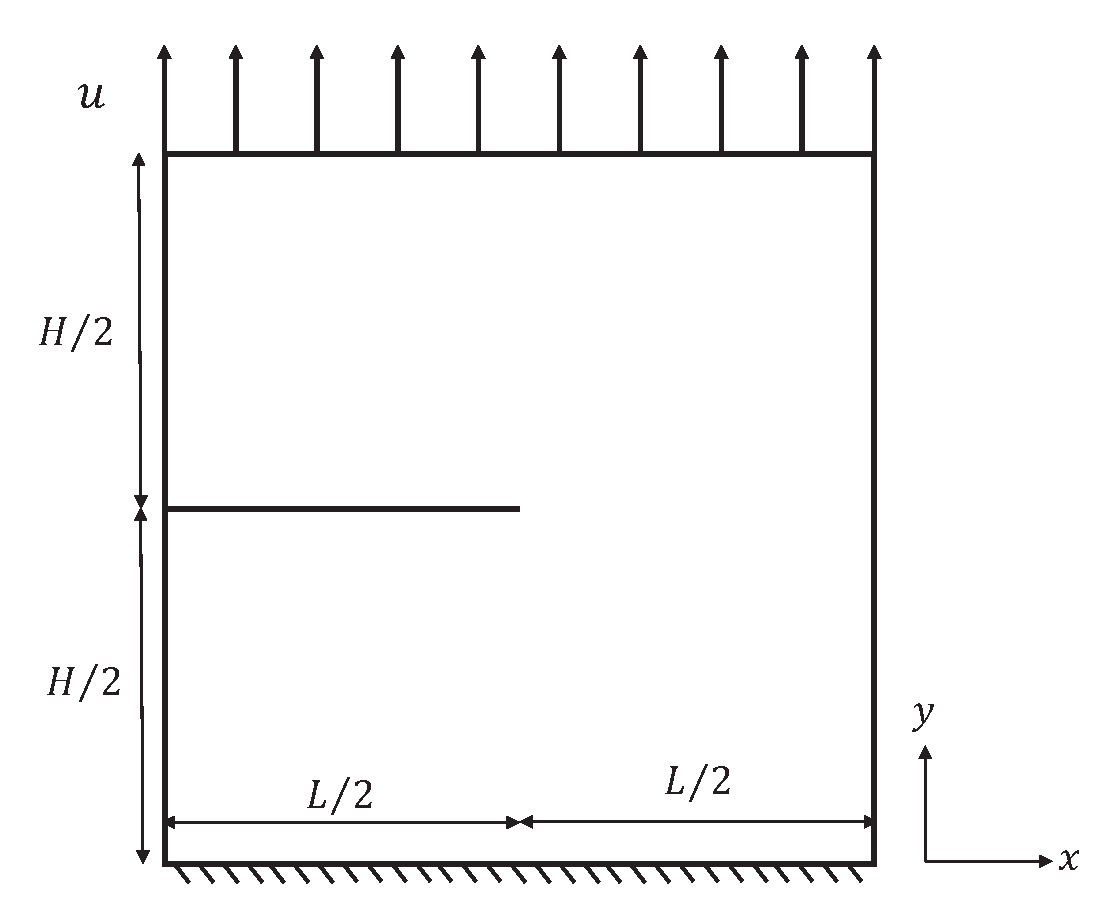
\includegraphics[width=80mm]{edgeNotch}
    \caption{Schematic of a cracked square plate (unit: mm) under a single-edge-notched tension test. 
    A monotonically increasing displacement with constant increments $\Delta\bm{u}=6\times 10^{-5}$ mm is applied on the top edge while the bottom edge is fixed.}
    \label{Fig:Notched_geometry}
\end{figure}

\begin{table}[htbp]
    \centering
    \caption{Cracked square plate under a tension test: Material parameters \cite{ambati2015review}}
    \begin{tabular}{l c c c}
    \hline 
         Parameters & symbol & unit& value \\
    \hline 
         Young's modulus & $E$ &MPa&  210$\times 10^{3}$\\
         Poisson's ratio & $\nu$ &$-$&  0.3\\
         Critical energy release rate & $g_c$ &MPa$\cdot$mm&  2.7\\
            \hline      
    \end{tabular}
    \label{Tab:Notched_input}
\end{table}

The resulting crack patterns at different stages of the deformation for two fixed regularization length scales $\ell = \ell_1 = 1\times 10^{-2}$ mm and $\ell = \ell_2=2 \times 10^{-2}$ mm are illustrated in Figure \ref{Fig:Notched_snapshots}. 
As expected, in both simulations, the fracture propagates straightforward to the end. This straight crack topology agrees well with the results in \cite{miehe2010thermodynamically}. Also as seen, the resulting crack pattern with the smaller $\ell$ looks sharper.

\begin{figure}[!htb]
    \centering
    \subfloat[]{
    
\includegraphics[width=0.4\textwidth]{snapshot_l2h_t92.eps}
    \label{Fig:Notched_lenght_scale_2h_i}}
    \subfloat[]{
    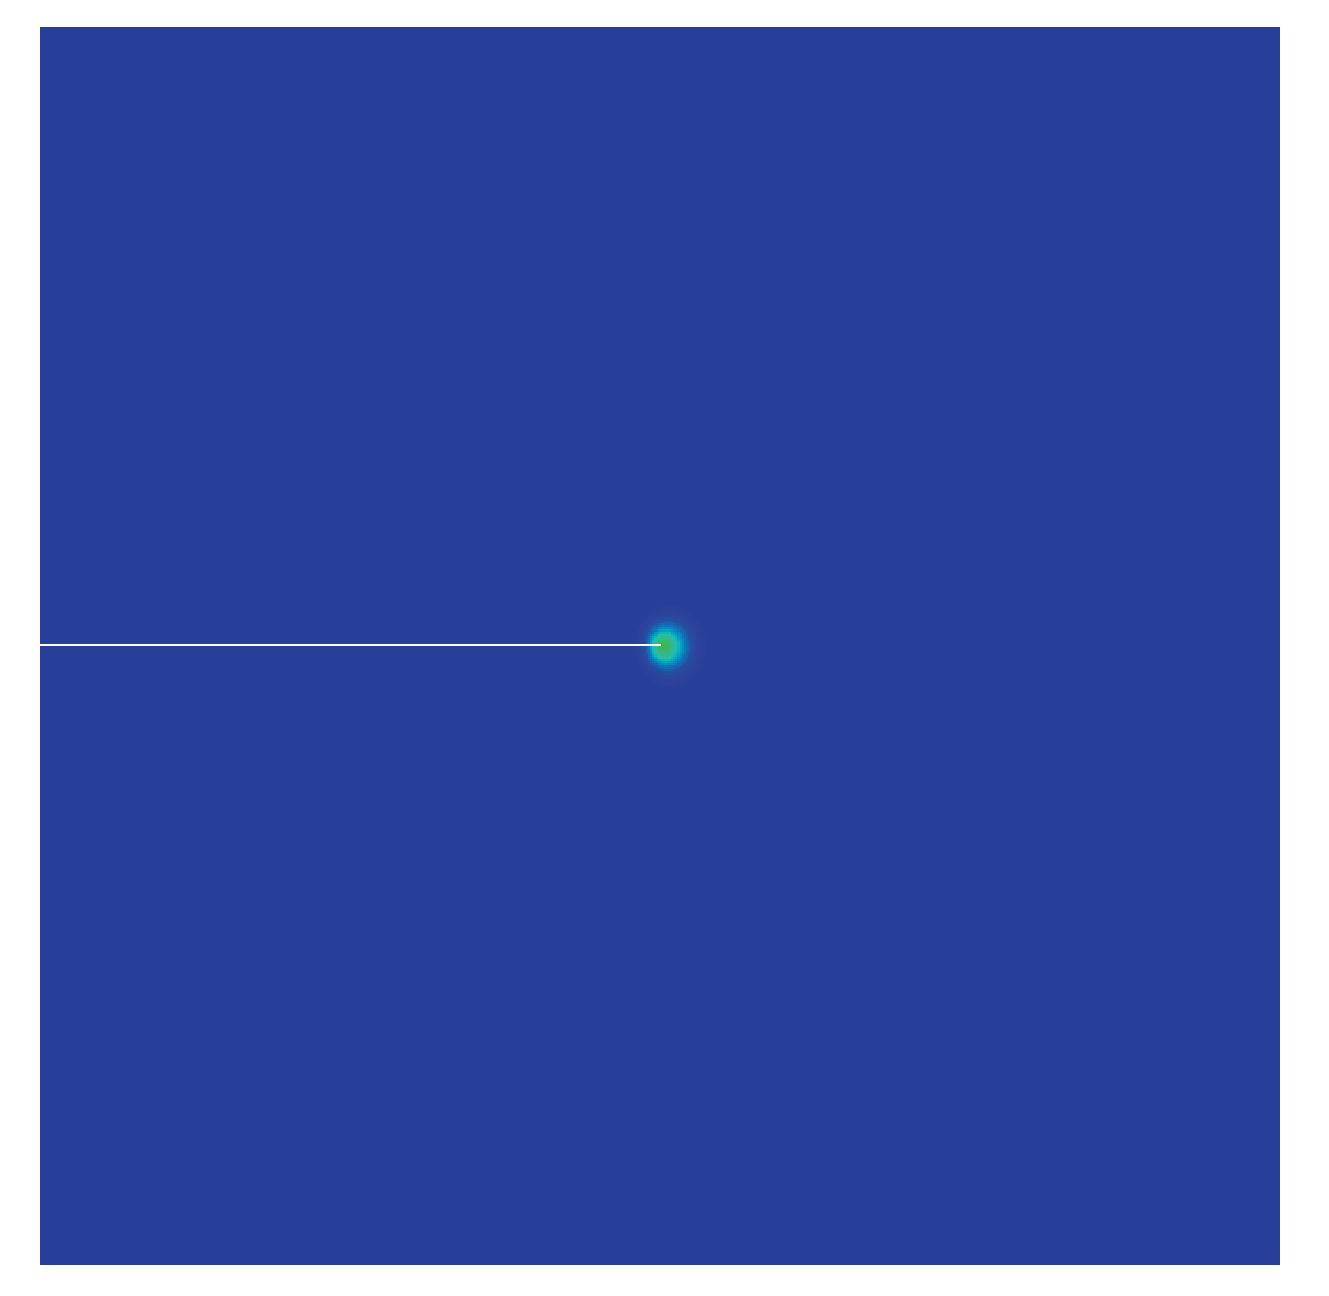
\includegraphics[width=0.4\textwidth]{snapshot_l4h_t92.eps}
    \label{Fig:Notched_lenght_scale_4h_i}}\\
    \subfloat[]{
    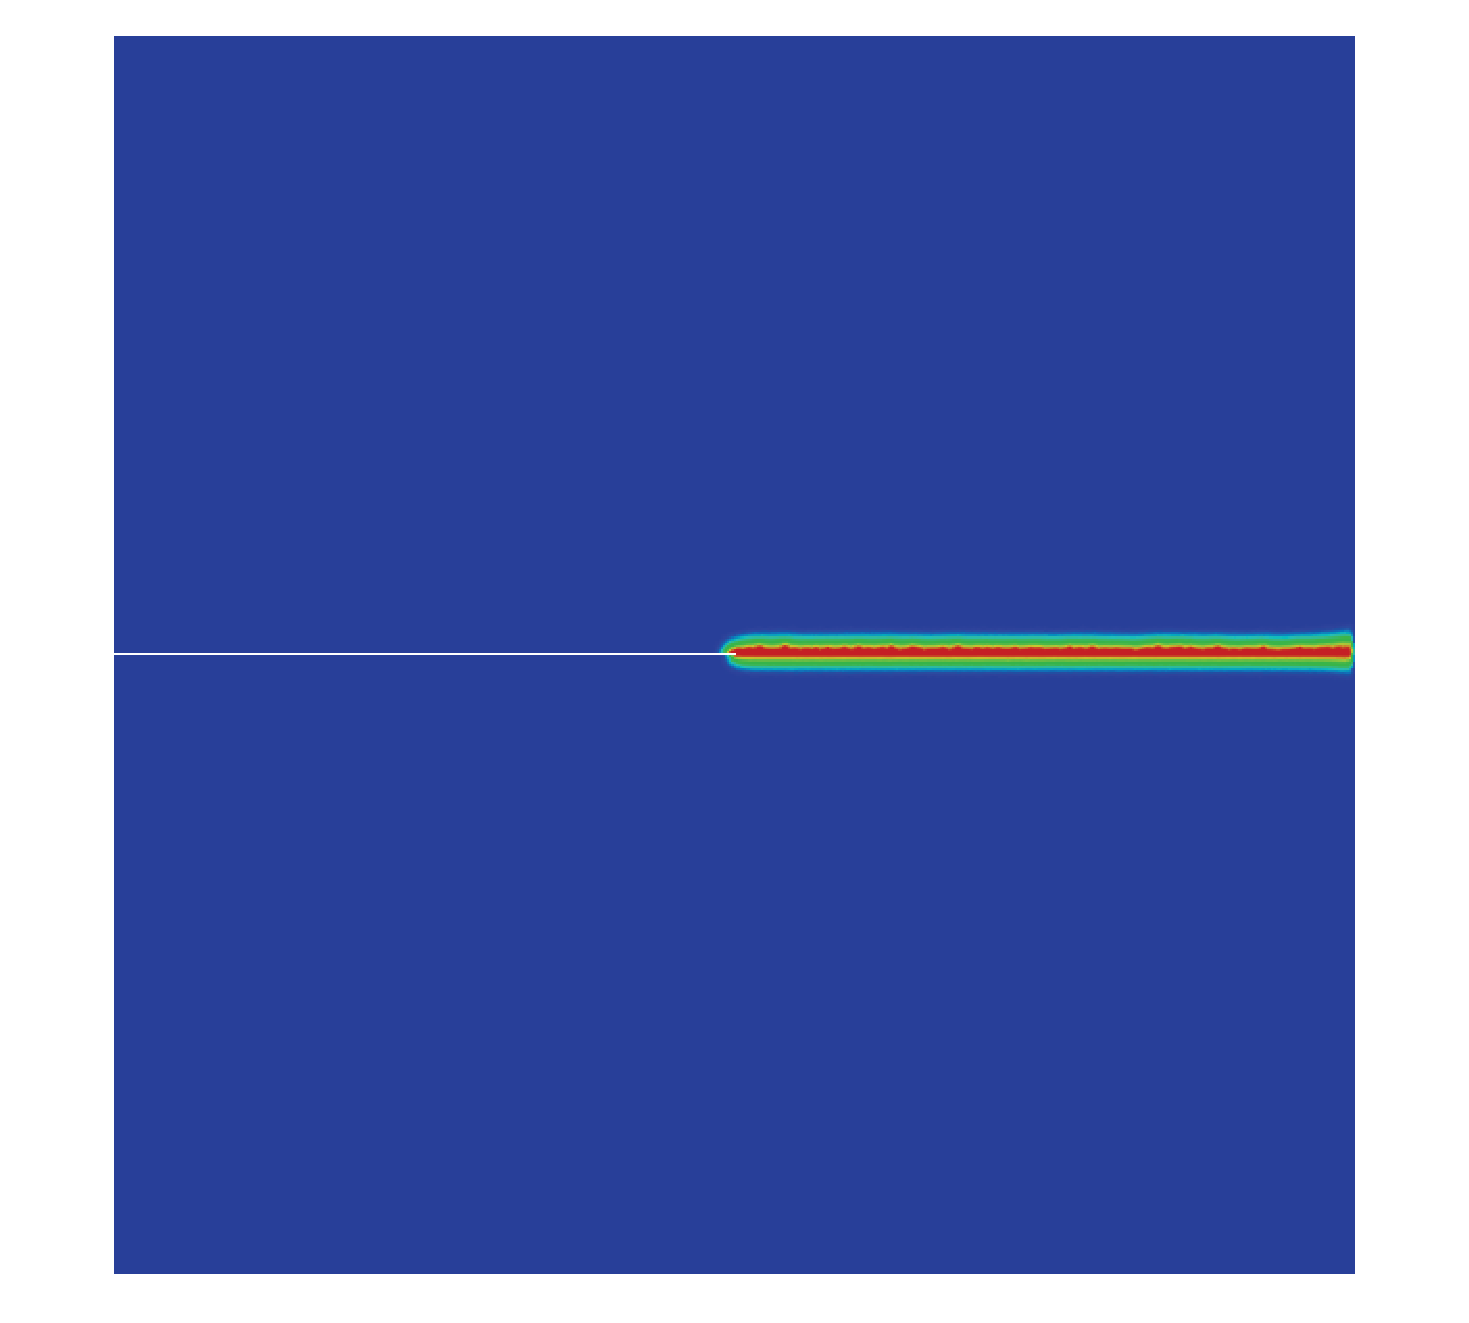
\includegraphics[width=0.4\textwidth]{snapshot_l2h_t93.eps}
    \label{Fig:Notched_lenght_scale_2h_ii}}
    \subfloat[]{
    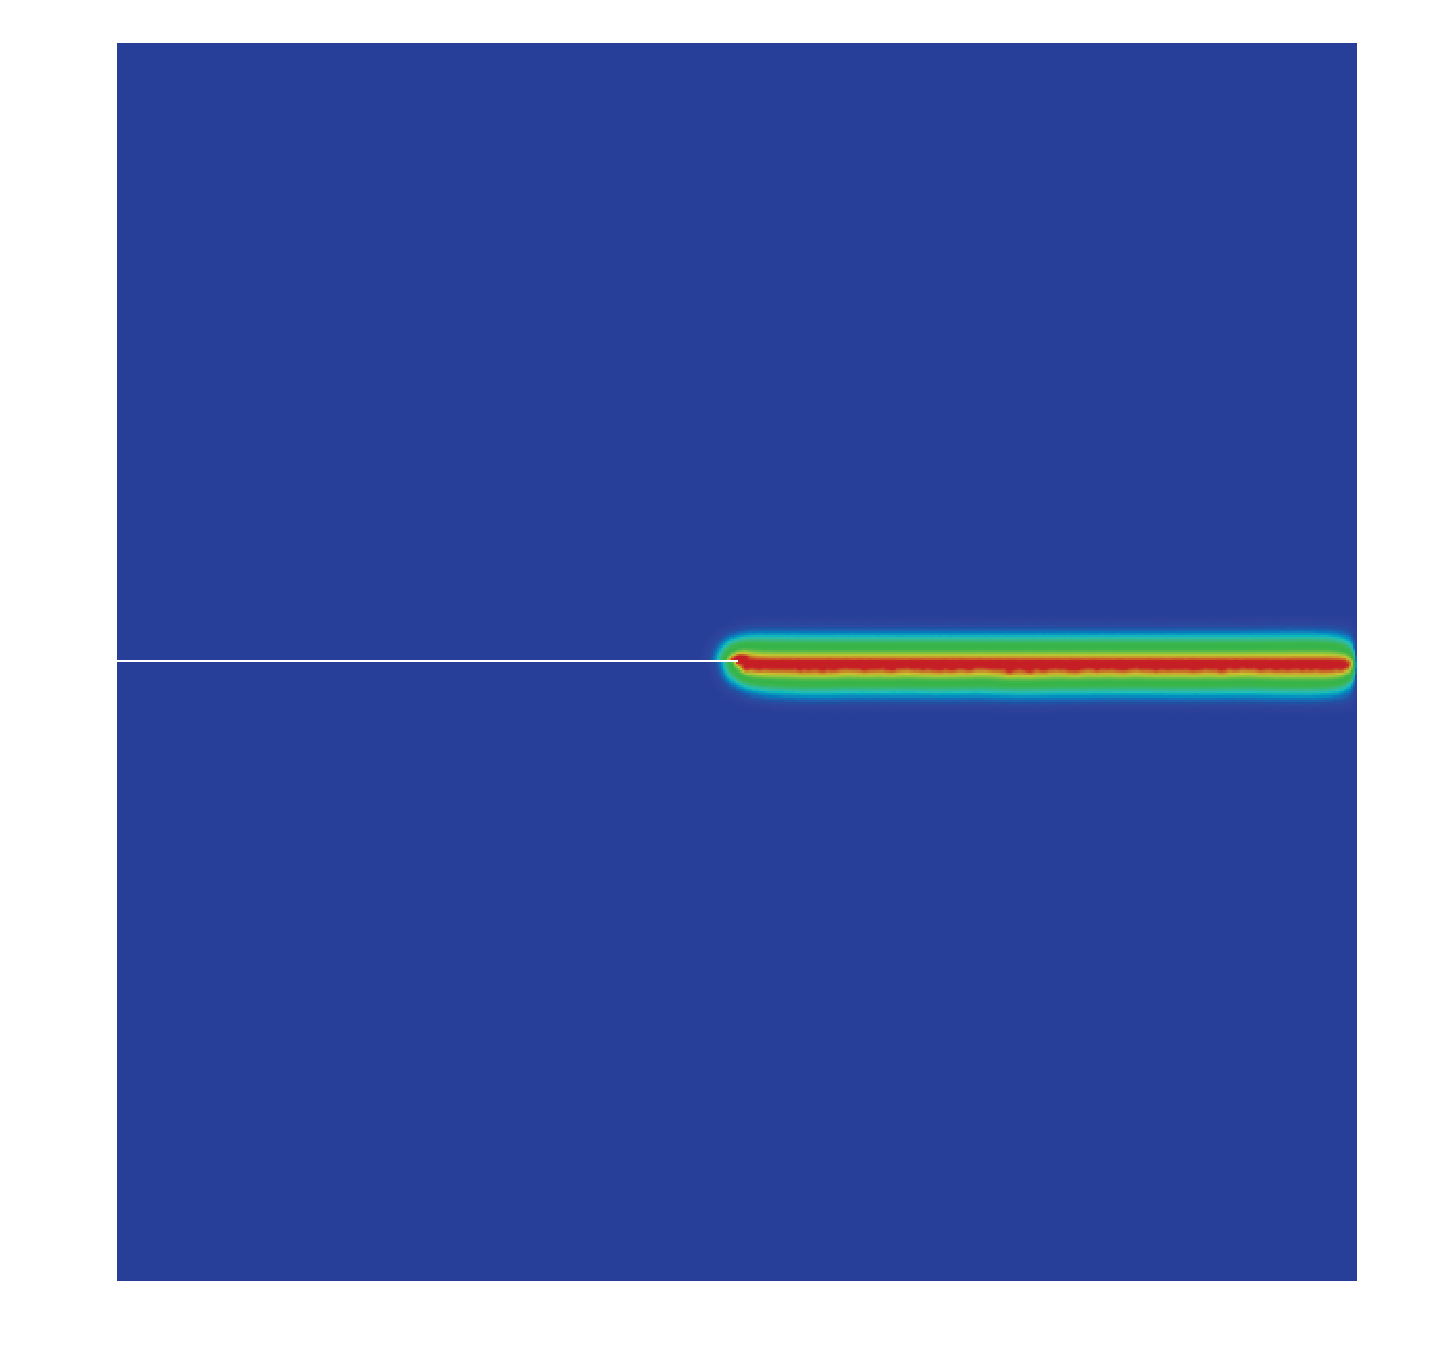
\includegraphics[width=0.4\textwidth]{snapshot_l4h_t93.eps}
    \label{Fig:Notched_lenght_scale_4h_ii}}\\
    \subfloat[]{
    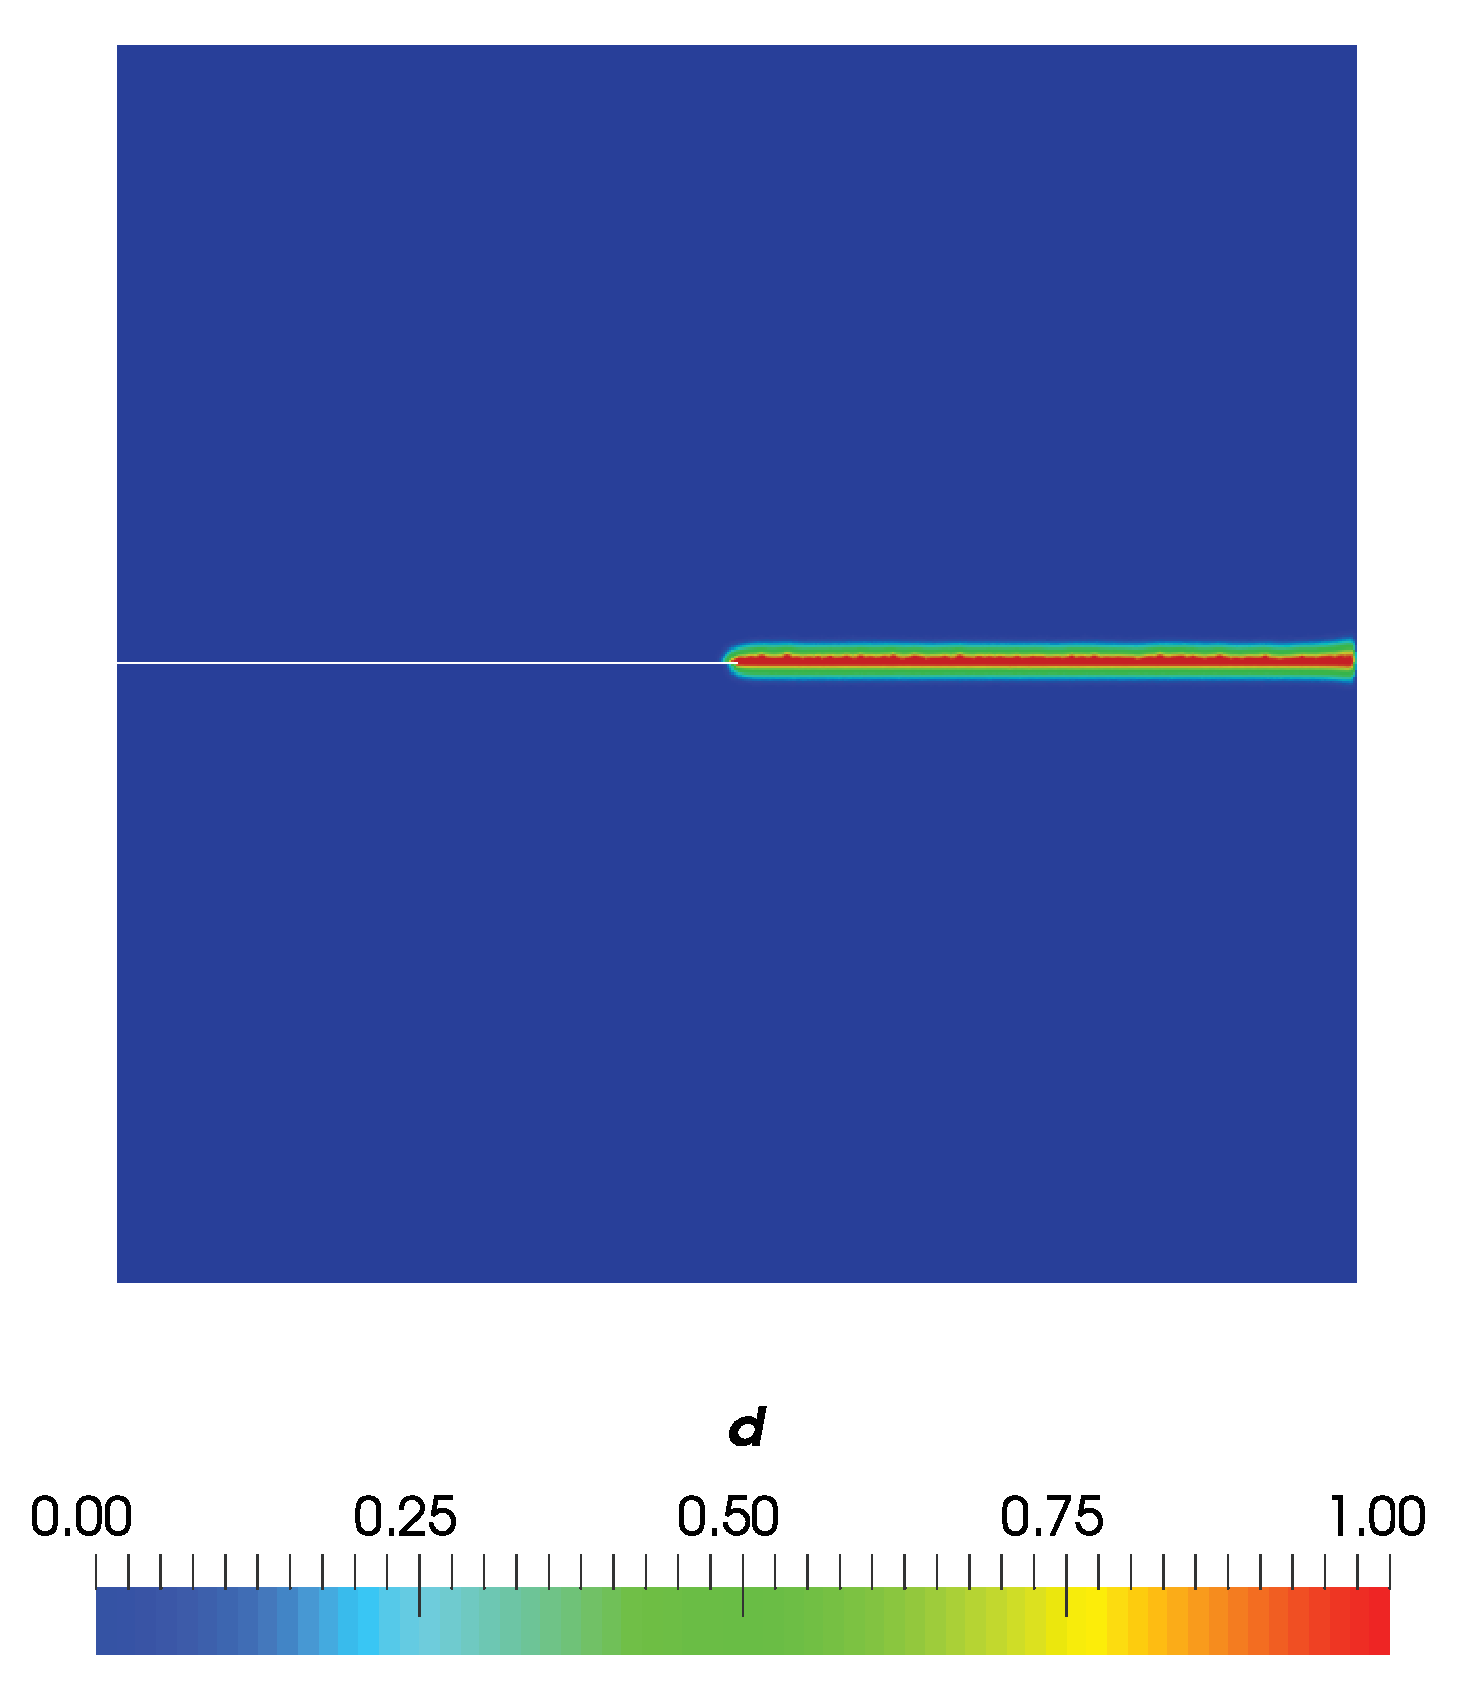
\includegraphics[width=0.4\textwidth]{snapshot_l2h_t99.eps}
    \label{Fig:Notched_lenght_scale_2h_iii}}
    \subfloat[]{
    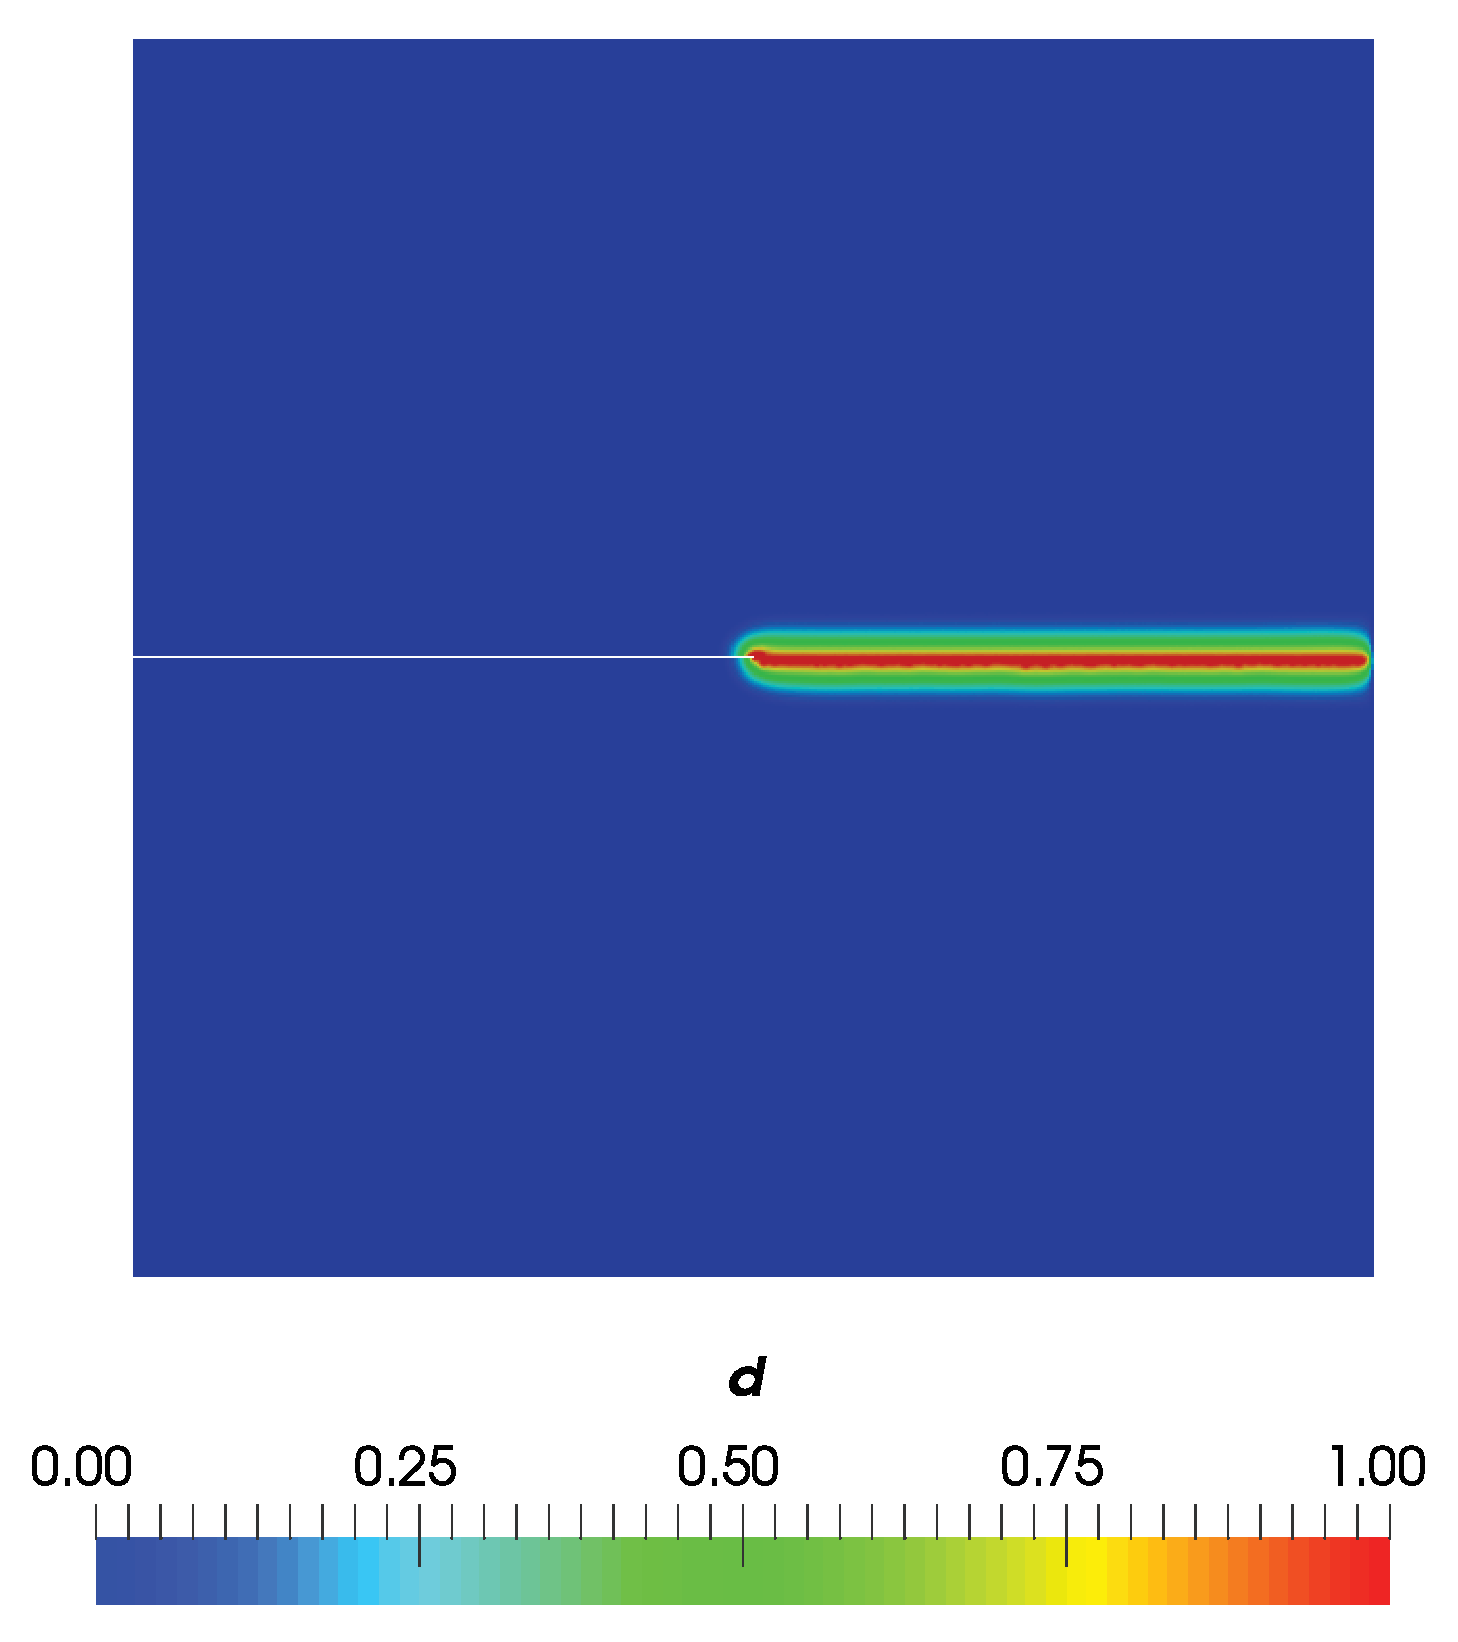
\includegraphics[width=0.4\textwidth]{snapshot_l4h_t99.eps}
    \label{Fig:Notched_lenght_scale_4h_iii}}

    \caption{Cracked square plate under a tension test {with two different regularization length scales $\ell=\ell_1 = 10^{-2}$ mm $\approx 2h$ (left) and $\ell=\ell_2 = 2\times 10^{-2}$ mm $\approx 4h$ (right)}. Both simulations are done with 100 uniform time steps with $\Delta\bm{u}= 6 \times 10^{-5}$ mm (See also Table \ref{Tab:Notched_input} for the input values). Phase field contours at three different stages $\bm{u}=5.52 \times 10^{-3}$ mm (\ref{Fig:Notched_lenght_scale_2h_i},\ref{Fig:Notched_lenght_scale_4h_i}), $\bm{u}=5.58 \times 10^{-3}$ mm (\ref{Fig:Notched_lenght_scale_2h_ii},\ref{Fig:Notched_lenght_scale_4h_ii}), and $\bm{u}=6 \times 10^{-3}$ mm (\ref{Fig:Notched_lenght_scale_2h_iii},\ref{Fig:Notched_lenght_scale_4h_iii}) are shown in deformed configurations with the deformations scaled. The initial cracks are explicitly imposed, so in the deformed configuration it appears as a white line. As expected, we observe a straight crack pattern in both cases.
    }
    \label{Fig:Notched_snapshots}
\end{figure}

We also output the load-deflection curves for the two setups of Figure \ref{Fig:Notched_lenght_scale}. As seen, both models will result in similar trends. Hence, the effect of $\ell$ on the response is small in this range.

\begin{figure}[htbp]
    \centering
    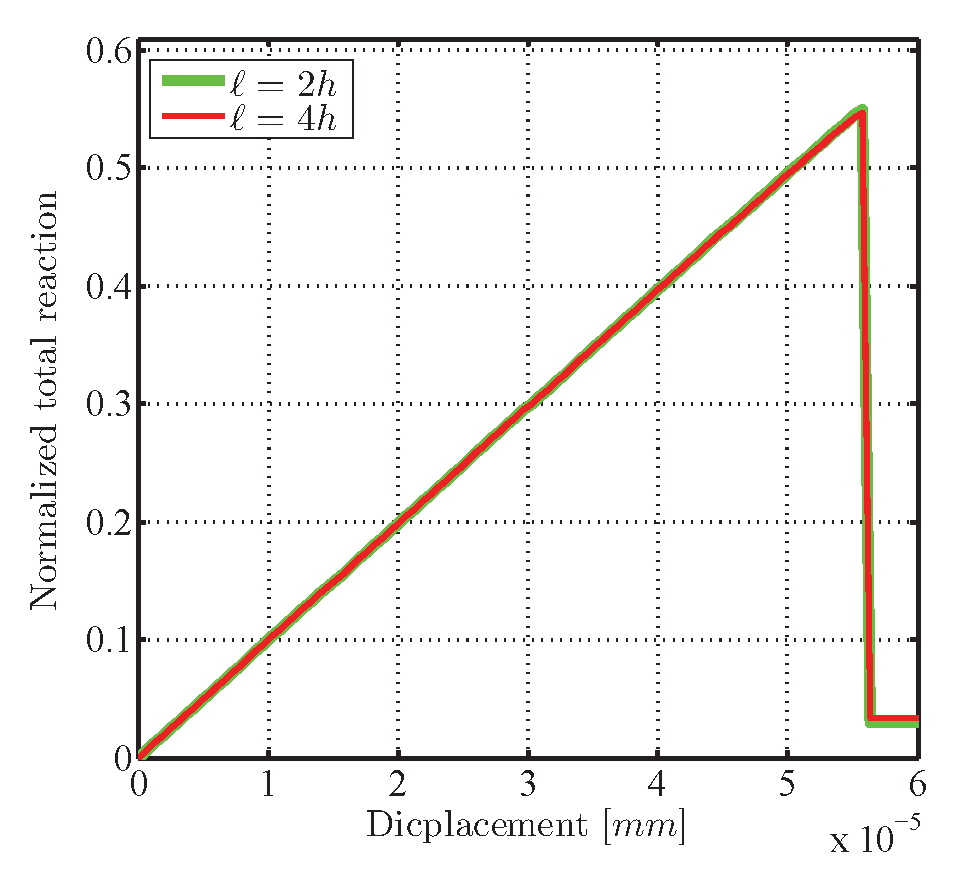
\includegraphics[width=0.6\textwidth]{Force_ELL_fracture}
    \caption{Cracked square plate under a tension test {with two different regularization length scales $\ell=\ell_1 =  10^{-2}$ mm $\approx 2h$ (red) and $\ell=\ell_2= 2\times 10^{-2}$ mm $\approx 4h$ (green)}. Load-deflection curves for both $\ell_1$ and $\ell_2$ are obtained. Both simulations are done with 100 load steps with $\Delta\bm{u}=6 \times 10^{-5}$ mm. The total reaction is normalized by the one in the case without any crack or phase field evolution. Both models give rise to similar trends so the effect of changes in $\ell$ is small within this range. Note that the reaction highly decreases at the 93rd time step where the crack starts to propagate.}
    \label{Fig:Notched_lenght_scale}
\end{figure}

%In order to point out the effects that arise due to the choice of the methods $AT1$ or $AT2$, Figure \ref{Fig:Notched_law_model} depicts the obtained load-deflection curves. Note that here we take $\ell= \added{4h}$. \added{As seen, both methods result in similar trends, although the $AT1$ method is having the higher pick value.}

%\begin{figure}[htbp]
%    \centering
 %   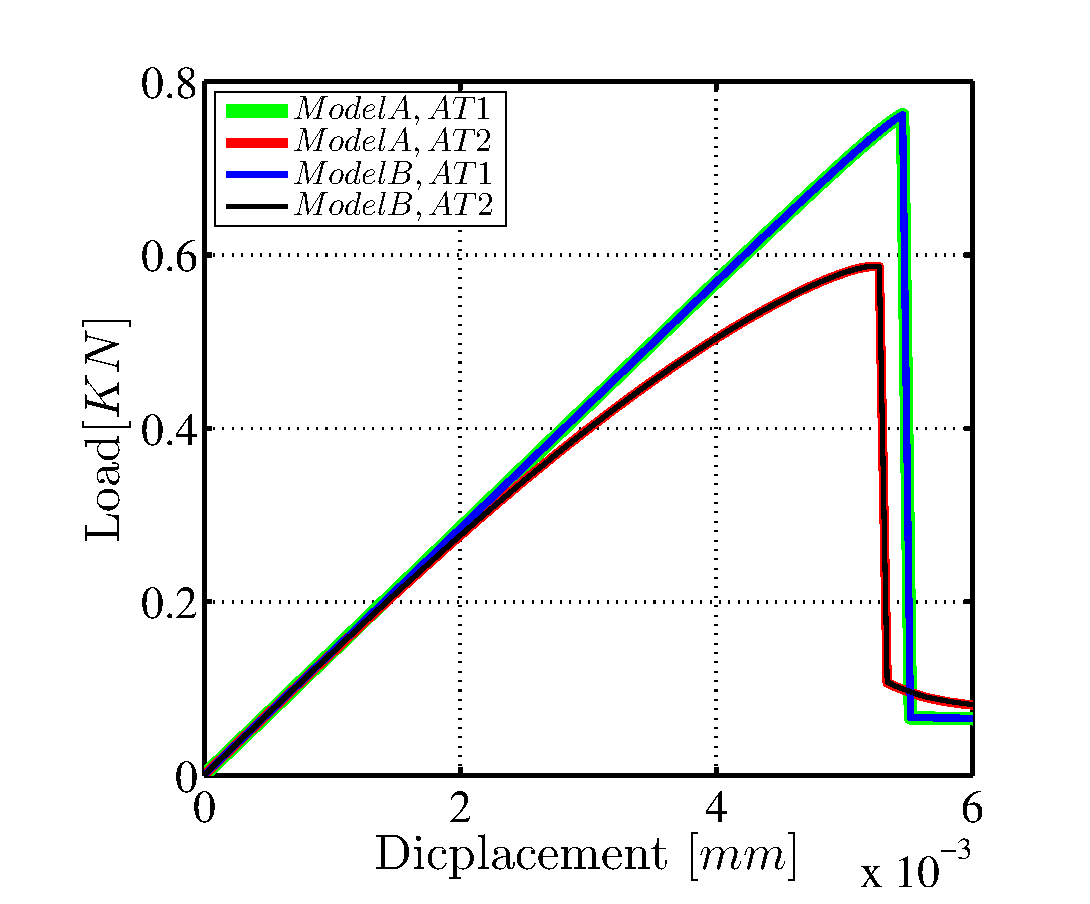
\includegraphics[width=100mm]{Force_LAW_MODEL_fracture.eps}
%    \caption{Cracked square plate under a tension test {with $\ell=\added{4h}~\text{mm}$.} Load-deflection curves for two different methods $AT1$ and $AT2$ are obtained. Both simulations are done with a number of \added{100} time steps with $\Delta\bm{u}= \added{0.006}~\text{mm}$. The total reaction is normalized by the one in the case without any crack or phase field evolution. The methods AT1 and AT2 show slightly different values while following similar trend. \added{Note that the total reaction highly decreases at the \dots-th time step where the crack starts to propagate.}}
%    \label{Fig:Notched_law_model}
%\end{figure}

\subsection{Poroelastic response of a borehole}
This example  aims to study the effect of fluid pressurization on the poroelastic response around the borehole.
It was first studied by {Detourney and Cheng} \cite{detournay1988poroelastic} (see also \cite{wang2018influence, lu2013microcrack}). Consider a plane strain hydraulic fracturing problem where there is a square plate containing a central borehole. The geometry and the loading conditions in this example are the same as Figure \ref{Fig:Gas_geometry}. The far-field \emph{in situ} stress is set to zero in this example. Note also that $d\equiv0$, i.e., there is no preexisting crack in the specimen and we do not allow for any nucleation of the fracture as the rock strength is assigned a very large value. A discretization with 28,140 standard $P_1$ elements is applied to the problem. To capture the high gradient of pressure near the borehole, the mesh is refined in that area so that an effective mesh size of $h\approx 0.15$ mm is adopted. The fluid is slightly compressible, and we set the fluid pressure in the borehole to $1$ MPa. The other material properties are prescribed according to Table \ref{Tab:Borehole_input}.

Here, the governing equation for the slightly compressible flow is written as follows \cite{detournay1988poroelastic}:
\begin{equation*}%\label{Eq:ap2}
   \begin{aligned}
        \partial_t p+ M \nabla \cdot \left(\frac{k_0}{\mu} \nabla p\right)=0
    \end{aligned}
\end{equation*}
where $M=E\left( 1-\nu\right) /[\left(1+\nu \right)\left(1-2\nu \right)]$ is called the constrained modulus.
%\todo[inline]{Vahid: Mostafa, please add the formula for $M$ in place of dots.\\Mostafa: it's added\\YS: It may be just $\lambda$ or the bulk modulus.\\Mostafa: It seems that $M $ is different from first Lame constant or bulk modulus.}
\begin{table}[htbp]
    \centering
    \caption{Poroelastic response of a borehole: Material parameters}
    \begin{tabular}{l c c c}
    \hline 
         Parameters & symbol & unit& value \\
    \hline 
         Young's modulus & $E$ &MPa&  6000\\
         Poisson's ratio & $\nu$ &$-$&  0.34\\
         Biot coefficient & $\alpha$ &$-$&  1.\\
         Permeability & $k_0$ &mm$^2$&  1$\times 10^{-12}$\\
            \hline      
    \end{tabular}
    \label{Tab:Borehole_input}
\end{table}

Figure \ref{Fig:Borehole_porepressure} shows the distribution
of pore pressure around the borehole for three values of dynamic viscosity $\mu$ at early time $t=0.1$ s. Note that the horizontal axis is $(r-r_0)/r_0$, ranging from $0$ to $0.25$ in the direction of $\theta= \pi/2$. The simulation results are then compared to the analytical solution by Detourney and Cheng \cite{detournay1988poroelastic}.

Figure \ref{Fig:Borehole_tangential_stress} depicts the effect of dynamic viscosity on the effective tangential stress in the vicinity of the borehole at early time $t=0.1$ s.%\todo{YS: Any conclusion?}

\begin{figure}[htbp]
    \centering
    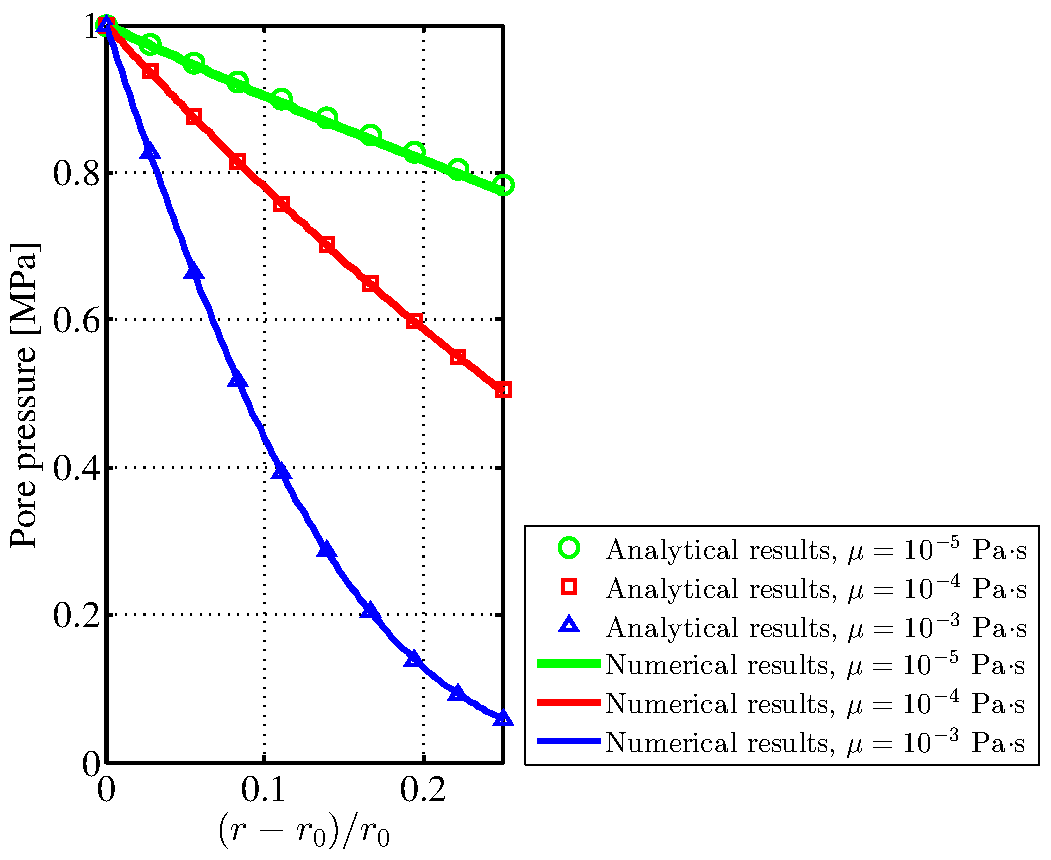
\includegraphics[width=0.8\textwidth]{verify_porepressure}
    \caption{Poroelastic response of a borehole. The distribution of pore pressure caused by fluid pressurization is shown around the borehole for three different dynamic viscosities $\mu$ at early time $t= 0.1$ s. As seen, the results are in good accordance with the analytical in \cite{detournay1988poroelastic}.}
    \label{Fig:Borehole_porepressure}
\end{figure}

\begin{figure}[htbp]
    \centering
    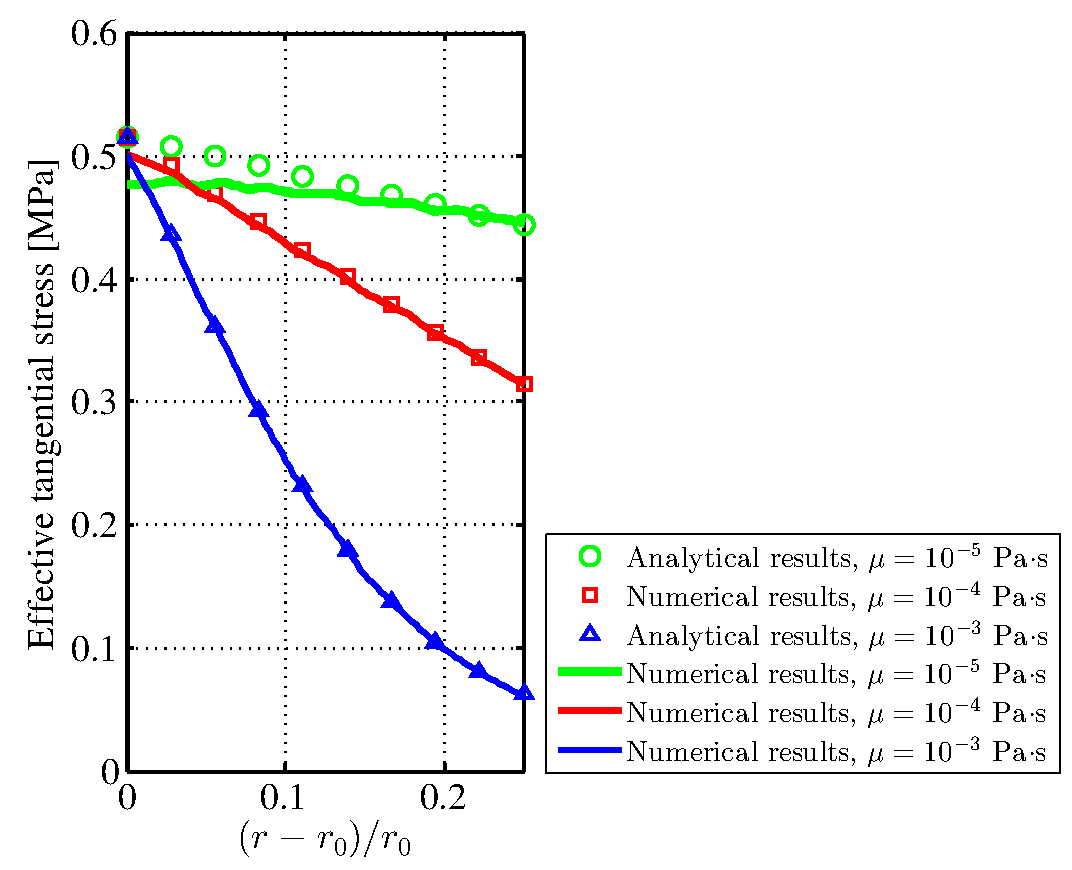
\includegraphics[width=0.8\textwidth]{verify_tangentialstress}
    \caption{Poroelastic response of a borehole. The effective tangential stress is plotted near the borehole for three different dynamic viscosities $\mu$ at early time $t=0.1$ s.}
    \label{Fig:Borehole_tangential_stress}
\end{figure}

\subsection{Computation of the crack opening displacement}
We now focus on a classical problem first solved by Sneddon and Lowengrouo \cite{SneddonLowengrub69} (see also \cite{bourdin2012variational}) that solves the opening displacement of a static line crack.

Consider a computational domain of $\Omega=4$ m $\times 4$ m with a preexisting line fracture of length $2a_0=0.4$ m, i.e., $\mathcal{C}=[1.8, 2.2]\times\{0\}$. To minimize the effect of the boundary conditions on the results, the domain size is much larger than the crack length ($L\gg 2a_0$).

The mechanical properties of the material are the Young's modulus $E=1000$ MPa, the Poisson's ratio $\nu=0$, and the fracture toughness $g_c=1$ MPa$\cdot$s.

We impose zero displacements on the external boundary of $\Omega$. Also we set $d=1$ on prescribed (initial) fracture and $d=0$ on the external boundary of $\Omega$. A monotonically increasing pressure is applied on the upper and lower faces of fracture with the magnitude $p=1$ MPa. Figure \ref{Fig:Sneddon_geometry} depicts the geometry and boundary conditions.

\begin{figure}
    \centering
    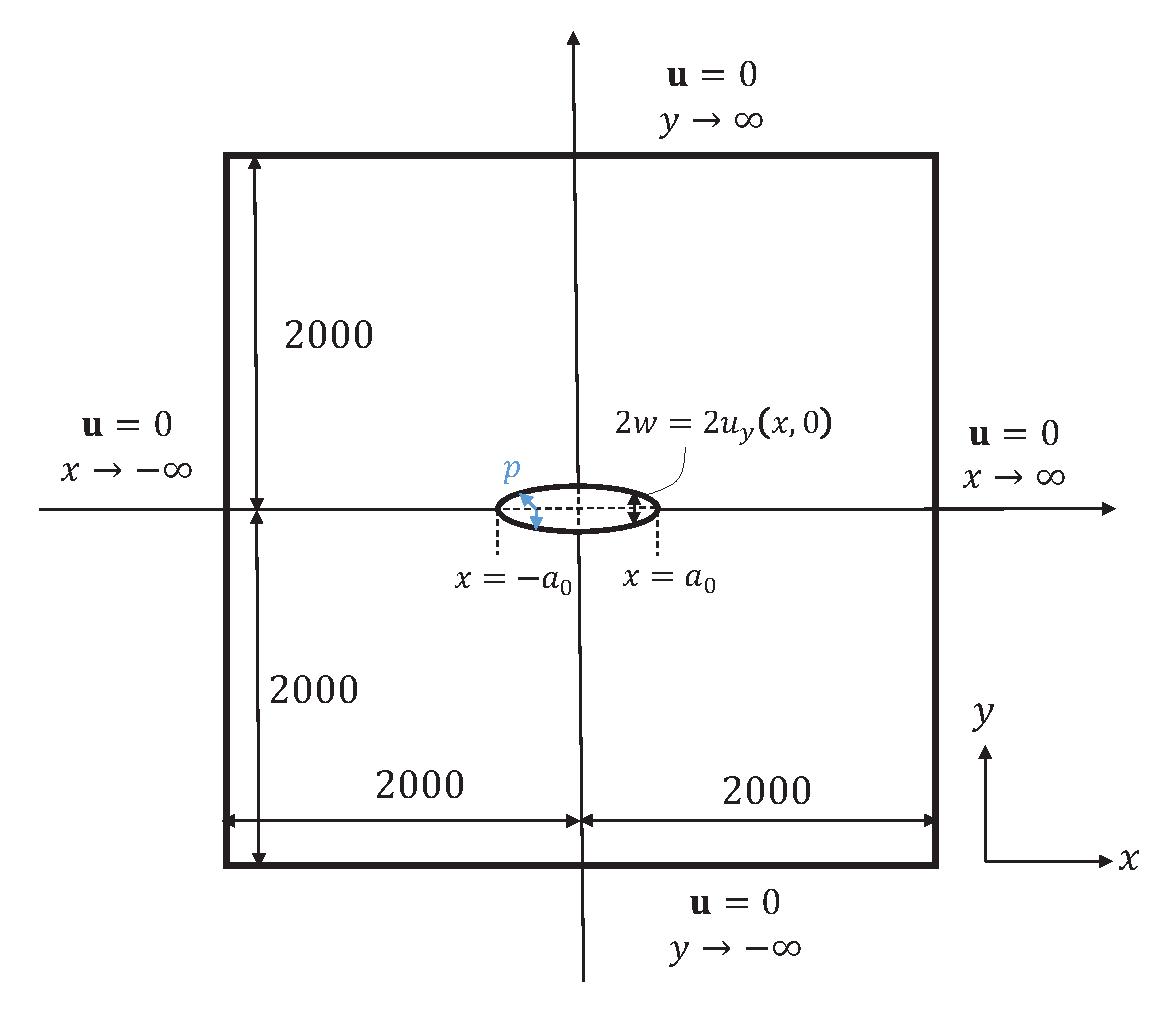
\includegraphics[width=0.8\textwidth]{centerCrack_sneddon.eps}
    \caption{Computation of the crack opening displacement. Schematic view of the deformed line crack in a two dimensional domain.}
    \label{Fig:Sneddon_geometry}
\end{figure}

%\todo{Mostafa: rewrite this part, these two paragraphs are a part of a PhD theses. \cite{Chukwudozie-2016a}}
 
%\paragraph*{Sneddon's 2D benchmark with constant pressure.}  This section simulates the deformation of a static line crack in an infinite two dimensional domain. This is the classic problem solved by Sneddon and Lowengrub (1969). The material is composed of a homogeneous isotropic. The domain is under plain strain conditions and the boundary conditions on the material is such that displacement and stresses vanish at infinity while the crack surface is acted upon by a uniform pressure p.  For the condition where the crack is found in the region defined by $y = 0$, $-l_0\le x \le l_0$, Sneddon and Lowengrub (1969) derived the following analytical expression for the crack opening displacement in the y-direction.
%\begin{equation} \label{eq: sneddon_opening}
%u_y(x,0)= \dfrac{2(p-\sigma_0) l_0}{E'}\sqrt{1-\dfrac{x_0}{l_0}}
%\end{equation}
%where $E'=\dfrac{E}{1-\nu^2}$. The fracture displacement profile is elliptic as evident from Equation \eqref{eq: sneddon_opening}. Thus, the fracture
%\begin{equation*}
% V_f=\pi \dfrac{2(p-\sigma_0) l_0^2}{E'}
%\end{equation*}

%\paragraph*{Compute the fracture width and volume.}  
Bourdin \emph{et al.}~\cite{BourdinCFRAC13} proposed a formula to compute the fracture aperture as:
\begin{equation*}
    w=\mathbf{u}\cdot n_{\Gamma} \simeq \int_{s} \mathbf{u} \cdot \nabla d \, dx.
\end{equation*}
Then, the fracture volume is calculated by integrating the fracture aperture along the fracture's path:
\begin{equation*}
    V_f= \int_{\Gamma} w \, ds \simeq \int_{\Omega} \mathbf{u} \cdot \nabla d \, d\Omega.
\end{equation*}

Figure \ref{Fig:Sneddon_opening} shows the {aperture} profile for different $h$ and $\ell$. The dash line in black represents the Sneddon's analytical solution \cite{SneddonLowengrub69}. Also, the crack volume computed by Sneddon's analytical solution and our numerical tests are summarized in Table \ref{Tab:Sneddon_volume}. %\todo{YS: Any conclusion?}

\begin{figure}[htbp]
    \centering
    \subfloat[]{
    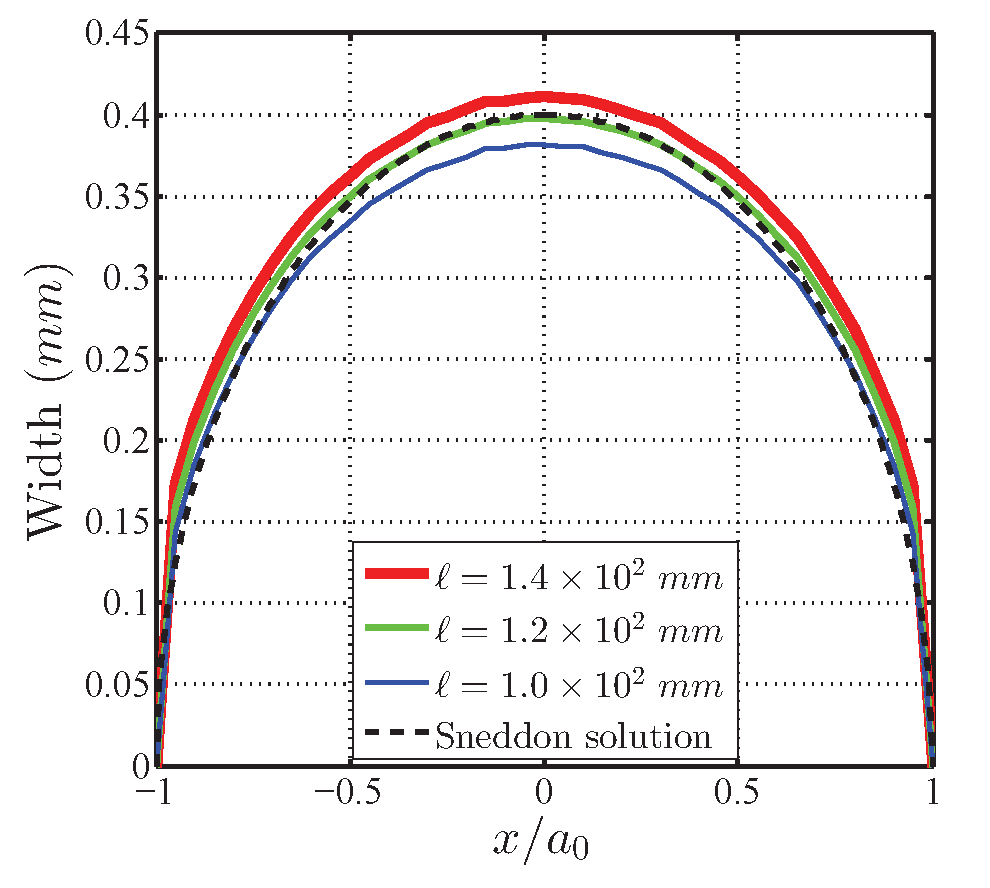
\includegraphics[width=0.5\textwidth]{width_ellVary.eps}
    \label{Fig:Sneddon_opening_ell}}
    \subfloat[]{
    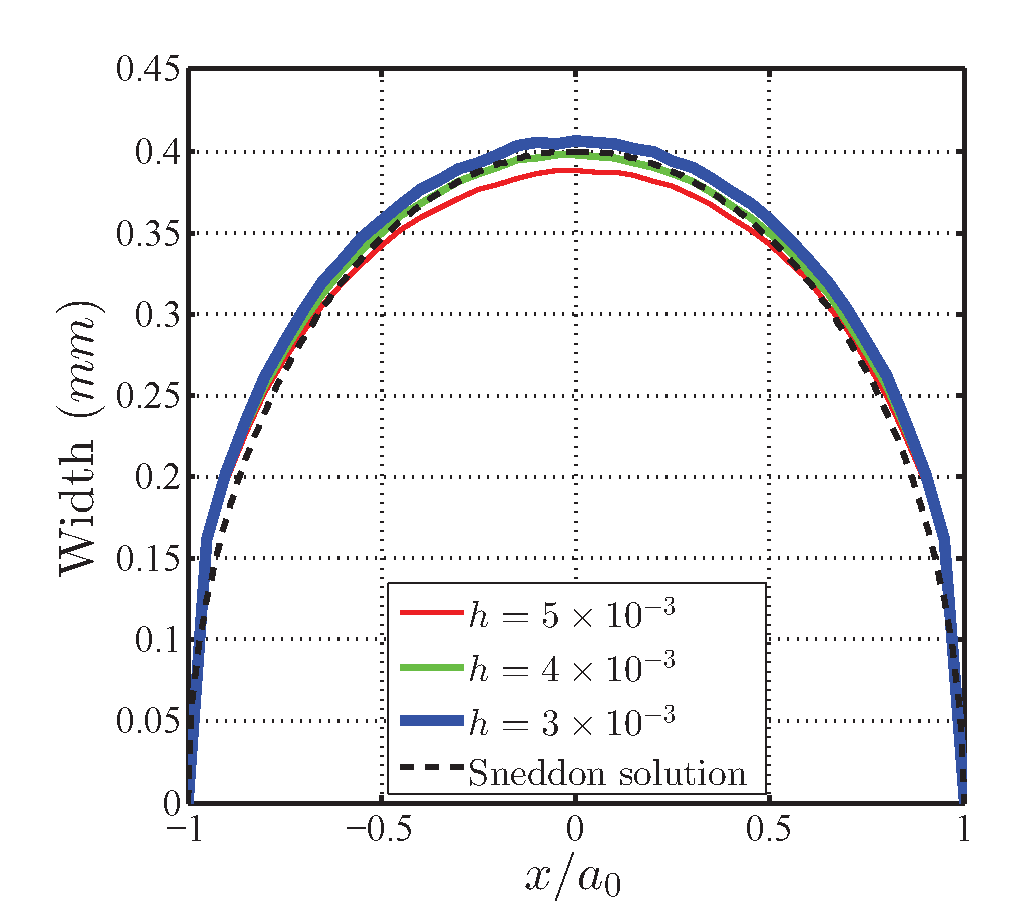
\includegraphics[width=0.5\textwidth]{width_hVary.eps}
    \label{Fig:Sneddon_opening_h}}    
    \caption{Computation of the crack opening displacement. We output the results for (\ref{Fig:Sneddon_opening_ell}) various $\ell$ with $h=4$ mm and (\ref{Fig:Sneddon_opening_h}) various $h$ with $\ell=1.2\times 10^{2}$ mm, and compare them with Sneddon's analytical solution \cite{SneddonLowengrub69}.}
    \label{Fig:Sneddon_opening}
\end{figure}

%\begin{figure}[htbp]
   % \centering
   % \includegraphics[width=0.7\textwidth]{centerCrackOpening.eps}
   % \caption{Phase field profile for center pressurized fracture, where $h=5  \times 10^-3~ \text{mm}$ and $\ell=4h$. }
 %   \label{Fig:opening_Pressrized_fracture_i}
%\end{figure}

\begin{table}[]
    \centering
    \caption{Crack volumes for different $\ell$ for numerical tests and analytical solution ($h=4\text{mm}$).}
    \begin{tabular}{l  c c c}
    \hline 
         $\ell$ (mm)  &1.4$\times 10^{2}$ & 1.2$\times 10^{2}$ &1.0$\times 10^{2}$\\
    \hline 
         Numerical fracture volume (mm$^2$) & 2.89$\times 10^{2}$ & 2.75$\times 10^{2}$  & 2.60$\times 10^{2}$\\
         Analytical fracture volume (mm$^2$) &2.51$\times 10^{2}$\\
    \hline      
    \end{tabular}
    \label{Tab:Sneddon_volume}
\end{table}

%\todo[inline]{Mostafa to vahid: please check the 3rd numerical example of \cite{wheeler2014augmented} to get more information about interaction example}
%\subsection{\added{Interaction of pressurized fractures}}
%\added{As the first example we conduct the interaction of pressurized fractures by phase field while the fluid pressure is increased. This example illustrates one of main abilities  of the phase field approach for interaction between fractures  without using any special geometry-adapted technique. }
%
%\added{Consider a computational domain of $\Omega=4$ m $\times 4$ m with three preexisting line fractures of length $2a_0=0.4$ m, i.e., $\mathcal{C}_c=[1.8, 2.2]\times\{0\}$, $\mathcal{C}_l=\{1.\}\times[1.8, 2.2]$, and $\mathcal{C}_r=\{3.\}\times[1.8, 2.2]$. To minimize the effect of the boundary conditions on the results, the domain size is much larger than the fracture length ($L\gg 2a_0$). A discretization with 19,368 standard $P_1$ elements is applied to the problem. To capture the high gradient of pressure near the fractures, the mesh is refined in that area so that an effective mesh size of $h\approx 20$ mm is adopted. while the length scale is $\ell=2h$. }
%
%\added{We keep all the mechanical properties of the material as in example of Section \ref{sec: AP-verification-opening}} %are the Young's modulus $E=1000$ MPa, the Poisson's ratio $\nu=0$, and the fracture toughness $g_c=1$ MPa$\cdot$s.}
%
%\added{We impose zero displacements on the external boundary of $\Omega$. Also we set $d=1$ on prescribed (initial) fractures and $d=0$ on the external boundary of $\Omega$. A monotonically increasing pressure is applied on the upper and lower faces of fracture with the magnitude $p=m\bar{p}$ where
%$\bar{p}=0.08$ MPa and $m=1, 2, \cdots500$ while  the governing equation is \ref{Eq:Dissipative_functional} for pressurized fracture. }
%
%\added{Figure \ref{Fig:Alpha_pressurized_interaction_snapshots} shows phase field diagram of interaction of pressurized fractures at different stages (\ref{Fig:Alpha0_pressurized_interaction}) $t=0$, (\ref{Fig:Alpha440_pressurized_interaction}) $t=0.88t_f$, and (\ref{Fig:Alpha499_pressurized_interaction}) $t=t_f$. The results show the center fracture at $t=0.880t_f$ starts to propagate  and at $t=0.882t_f$.  the center fracture interacts with vertical fractures (unstable fracture propagation).}
%
%
%\begin{figure}[htbp]
%    \centering
%    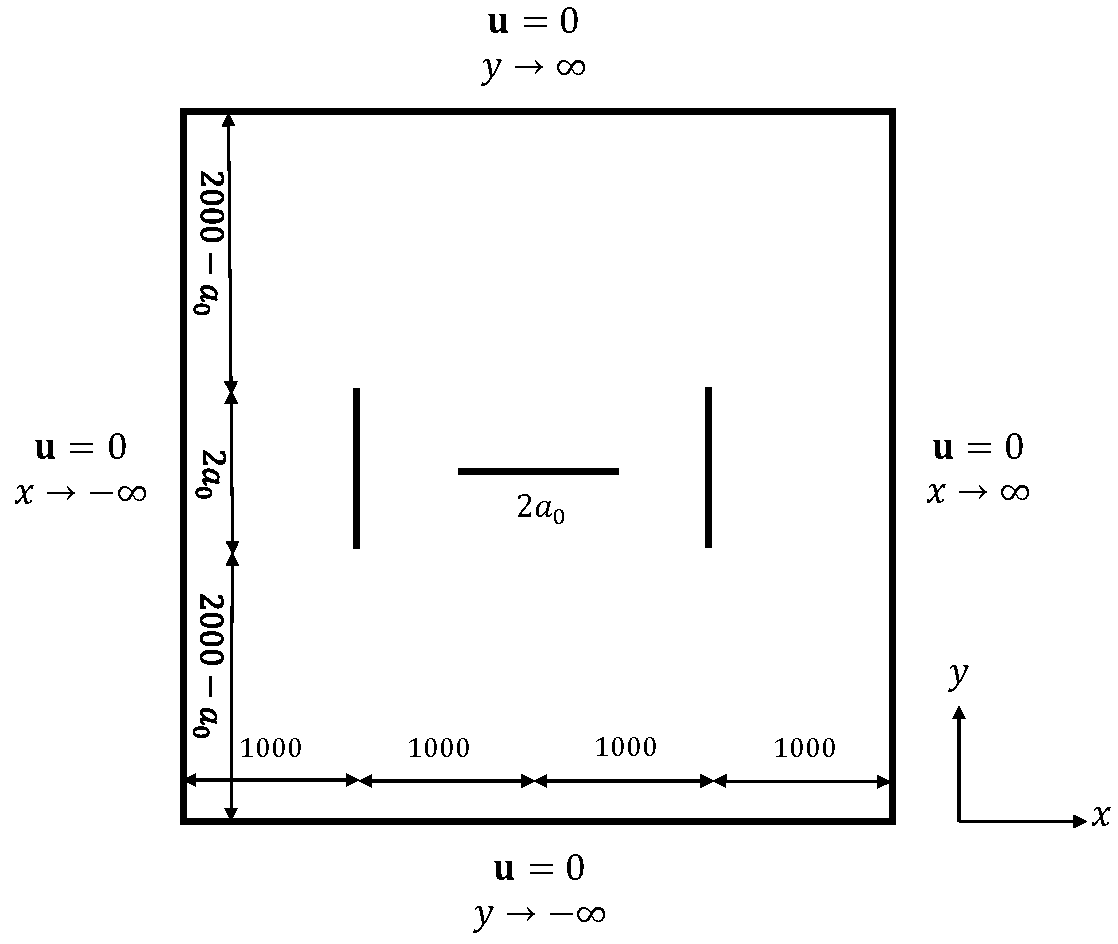
\includegraphics[width=0.8\textwidth]{Interaction_pressurized}
%    \caption{\added{Computation domain of interaction of pressurized fractures.}}
%    \label{Fig:Interaction_pressurized}
%\end{figure}
%
%\added{Figure \ref{Fig:Alpha_pressurized_interaction_snapshots} shows the  phase field contour of jointing fracture due to increasing fluid pressure.}
%
%\begin{figure}[htbp]
%\centering %
%\subfloat[]{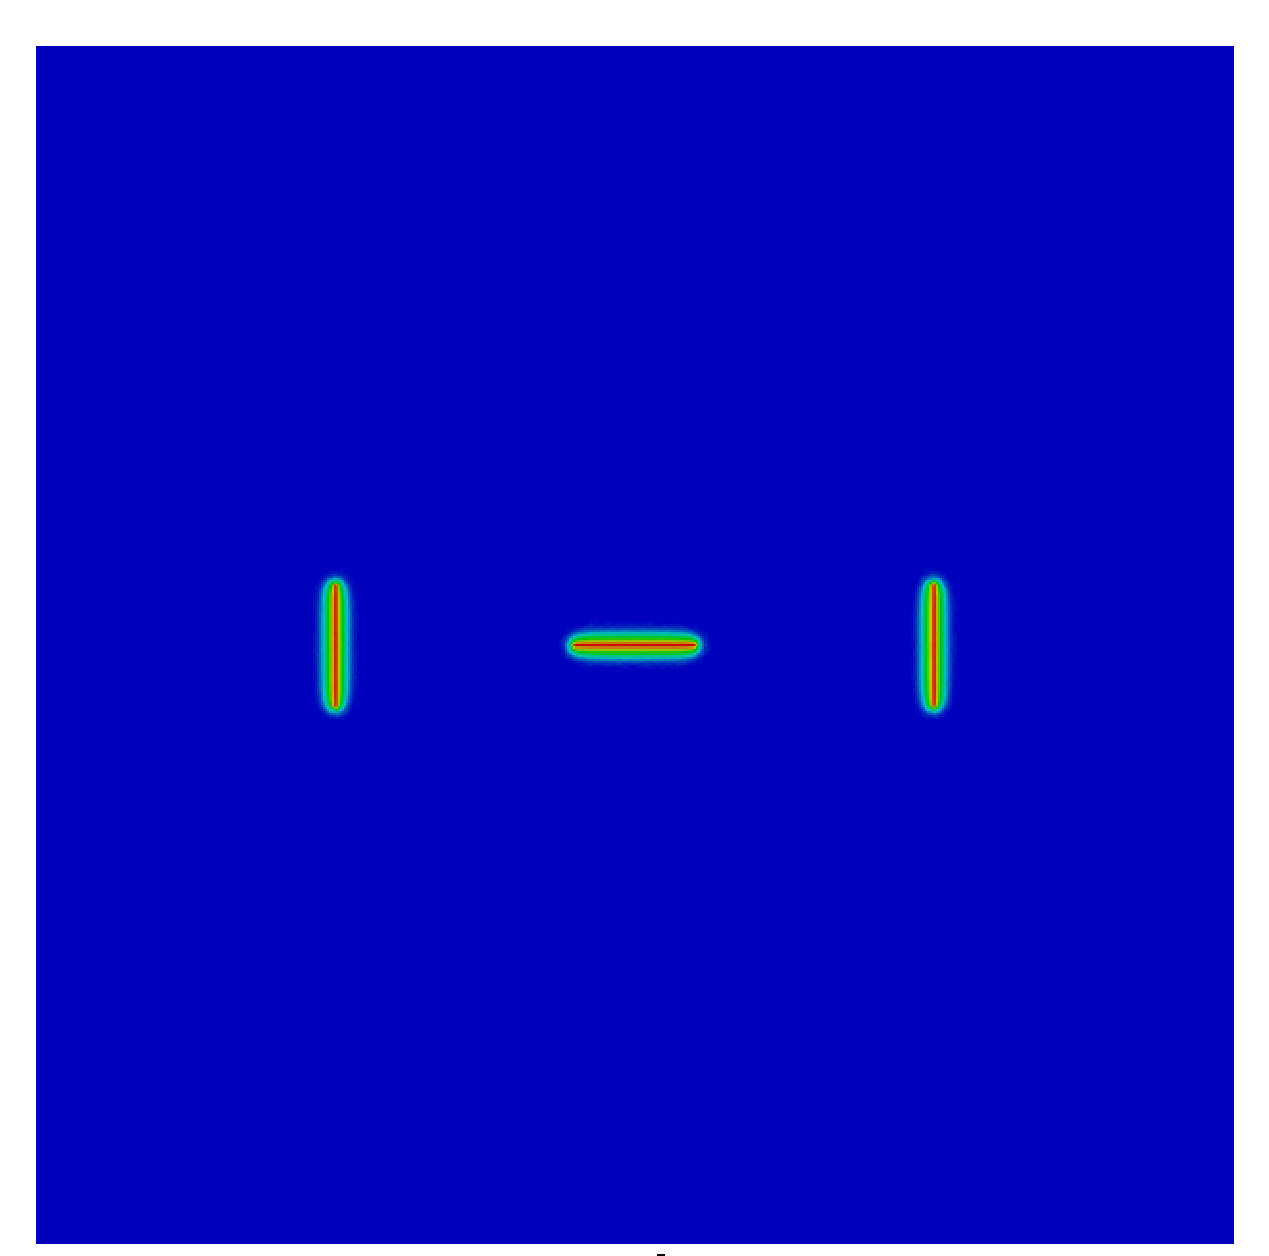
\includegraphics[width=65mm]{Alpha0_pressurized_interaction}\label{Fig:Alpha0_pressurized_interaction}}
%\\
%\subfloat[]{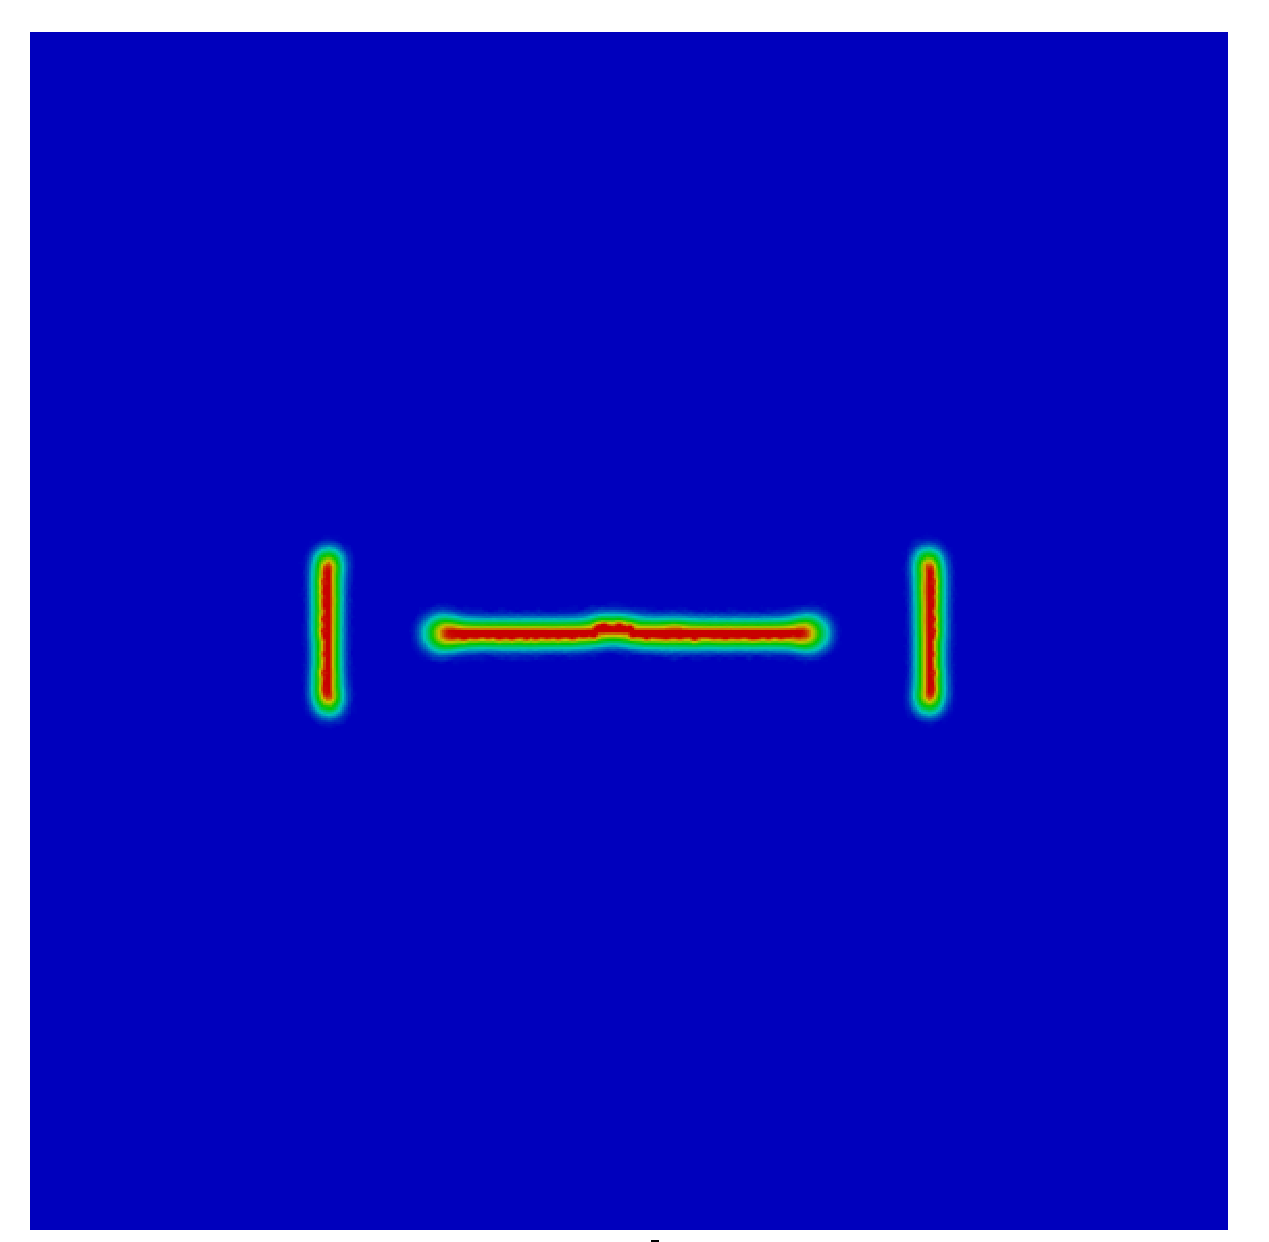
\includegraphics[width=65mm]{Alpha440_pressurized_interaction}\label{Fig:Alpha440_pressurized_interaction}}
%\\
%\subfloat[]{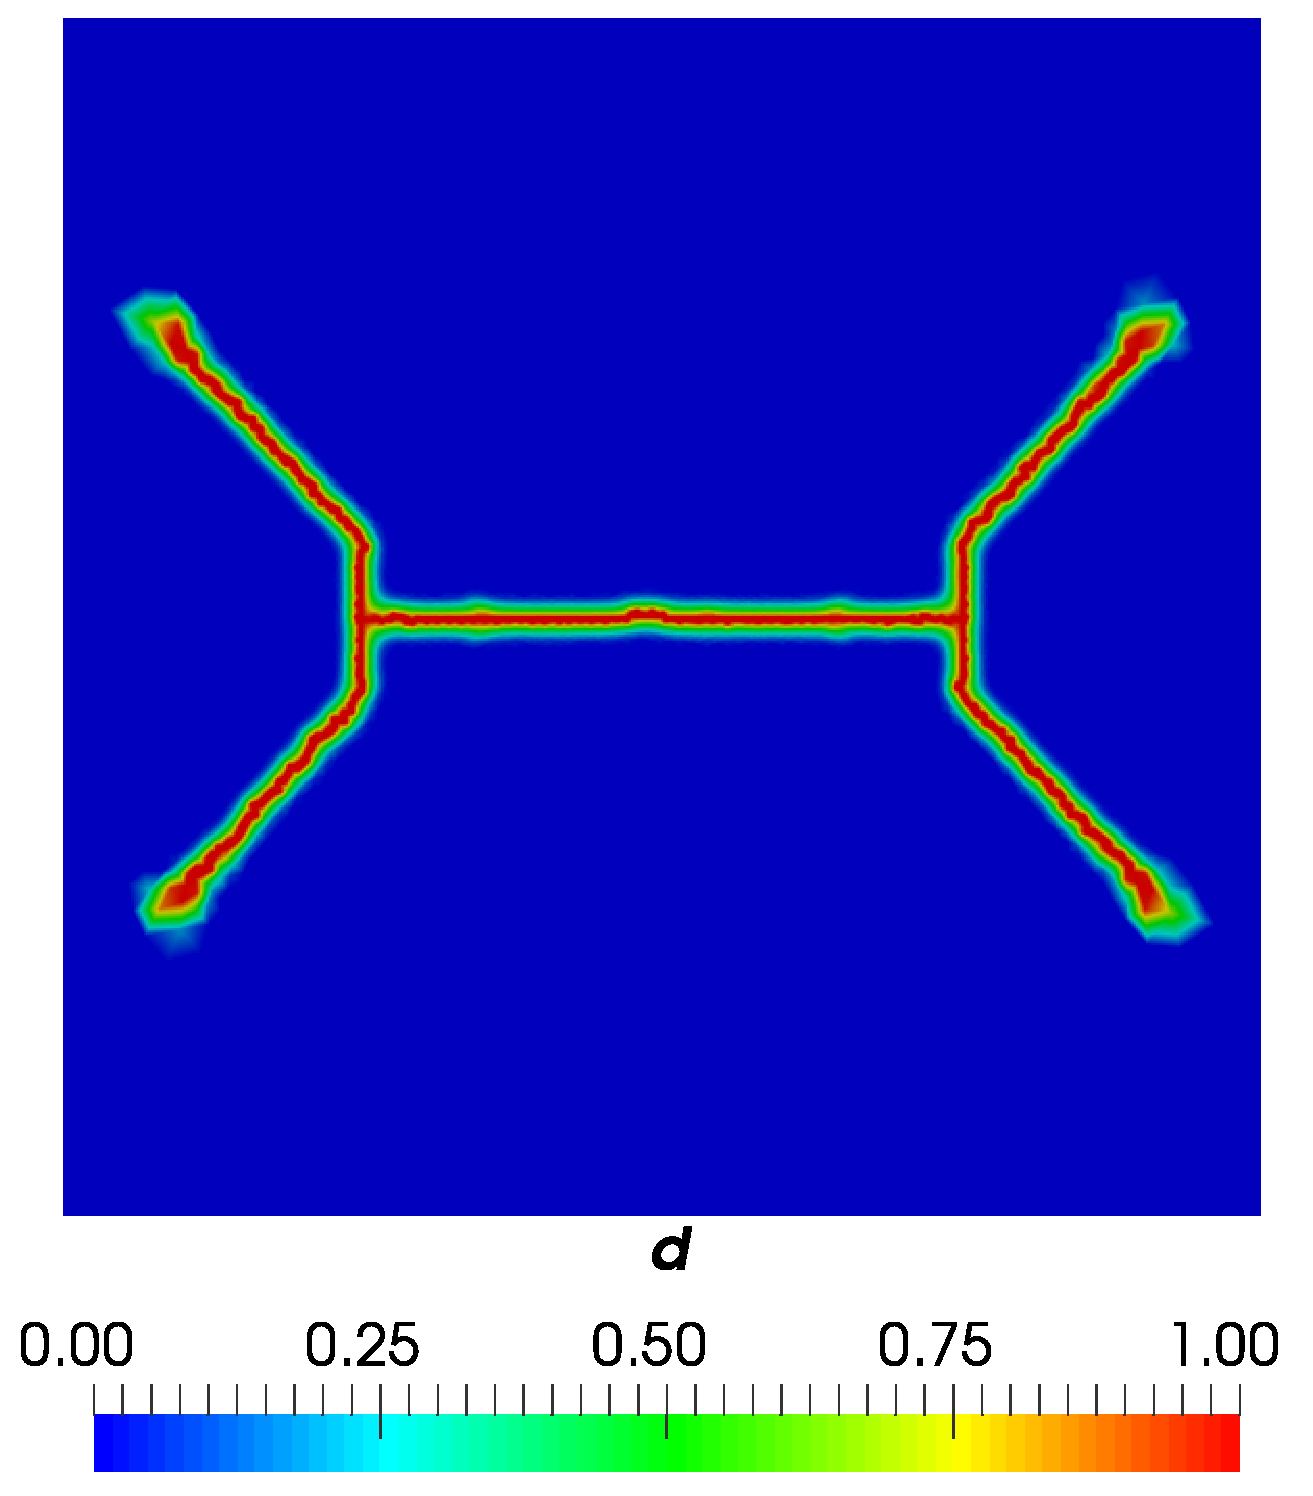
\includegraphics[width=65mm]{Alpha499_pressurized_interaction}\label{Fig:Alpha499_pressurized_interaction}}
%\caption{\added{Phase field diagram of interaction of pressurized fractures at different stages (\ref{Fig:Alpha0_pressurized_interaction}) $t=0$, (\ref{Fig:Alpha440_pressurized_interaction}) $t=0.88t_f$, and (\ref{Fig:Alpha499_pressurized_interaction}) $t=t_f$)}}
%\label{Fig:Alpha_pressurized_interaction_snapshots}
%\end{figure}

\subsection{\added{Increasing pressure leading to joining fractures}}
\added{This example motivated by Wheeler \emph{et al.}~\cite{Wheeler201469} demonstrates one major capability of the phase field approach that there is no need to track any complicated fracture geometry for joining fractures.}

\added{Consider a computational domain of $\Omega=(0,4.0)\times(0,4.0)$ (unit: m by m) containing two pre-existing %horizontal and vertical 
	line fractures with a length of $2a_0=0.4$ m, more precisely, $\mathcal{C}_h=[1.8, 2.2]\times\{0\}$ and $\mathcal{C}_v=\{2.6\}\times[1.8, 2.2]$. To minimize the effect of the boundary conditions on the results, the domain size is much bigger than the fracture length ($L\gg 2a_0$). A discretization with $19,368$ standard $P_1$ elements is applied such that an effective element size of $h\approx 20$ mm is obtained in the critical zone. Also, let $\ell=2h$. Figure \ref{Fig:Notched_geometry} depicts the geometric setup. A zero displacement is imposed on the boundary. Also, we set $d=1$ for the prescribed (initial) fractures, and $d=0$ on the boundary. A monotonically increasing pressure is applied on the upper and lower faces of the fracture with the magnitude $p=m\bar{p}$ where $\bar{p}=0.01$ MPa and $m=1, 2, \cdots, 115$.}

\begin{figure}[htbp]
	\centering
	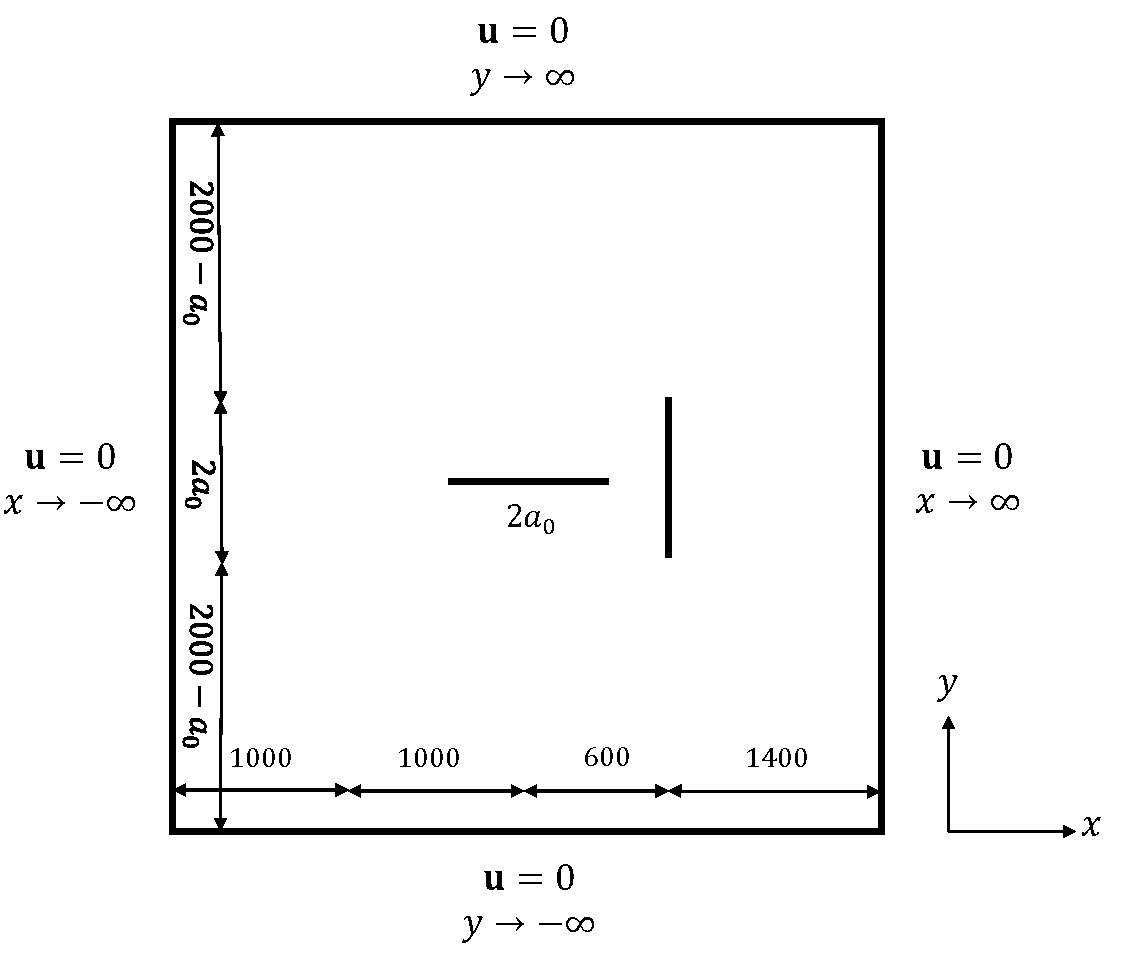
\includegraphics[width=0.8\textwidth]{Interaction_pressurized_2cracks}
	\caption{\added{Schematic of a square plate (unit: mm) with two pre-existing fractures.
			A monotonically increasing pressure with constant increments $p=m\bar{p}$ is applied on the fracture faces.}}
	\label{Fig:Notched_geometry}
\end{figure}

\added{Following \cite{Wheeler201469}, we adopt the values of the material parameters given in Table \ref{Tab:Join_input}.}

\begin{table}[htbp]
	\centering
	\color{blue}
	\caption{\added{Increasing pressure leading to joining fractures: Material parameters \cite{Wheeler201469}}}
	\begin{tabular}{l c c c}
		\hline 
		Parameters & symbol & unit& value \\
		\hline 
		Young's modulus & $E$ &MPa& 1.0\\
		Poisson's ratio & $\nu$ &$-$&  0.2\\
		Critical energy release rate & $g_c$ &MPa$\cdot$mm&  1.0\\
		\hline      
	\end{tabular}
	\label{Tab:Join_input}
\end{table}

\added{Figure \ref{Fig:Alpha_pressurized_interaction_snapshots} shows the phase field evolution at different load steps: (\ref{Fig:alpha_inter_0}) $m=1$, (\ref{Fig:alpha_inter_112}) $m=113$, (\ref{Fig:alpha_inter_113}) $m=114$, and (\ref{Fig:alpha_inter_114}) $m=115$. The results show that the horizontal fracture starts to propagate at $m=113$, and at $m=114$ it intesects the vertical fracture.
	Overall speaking the fracture paths agree with those in \cite{Wheeler201469}. Note the fracture propagation is unstable in this example.}

\begin{figure}[htbp]
\centering %
\subfloat[]{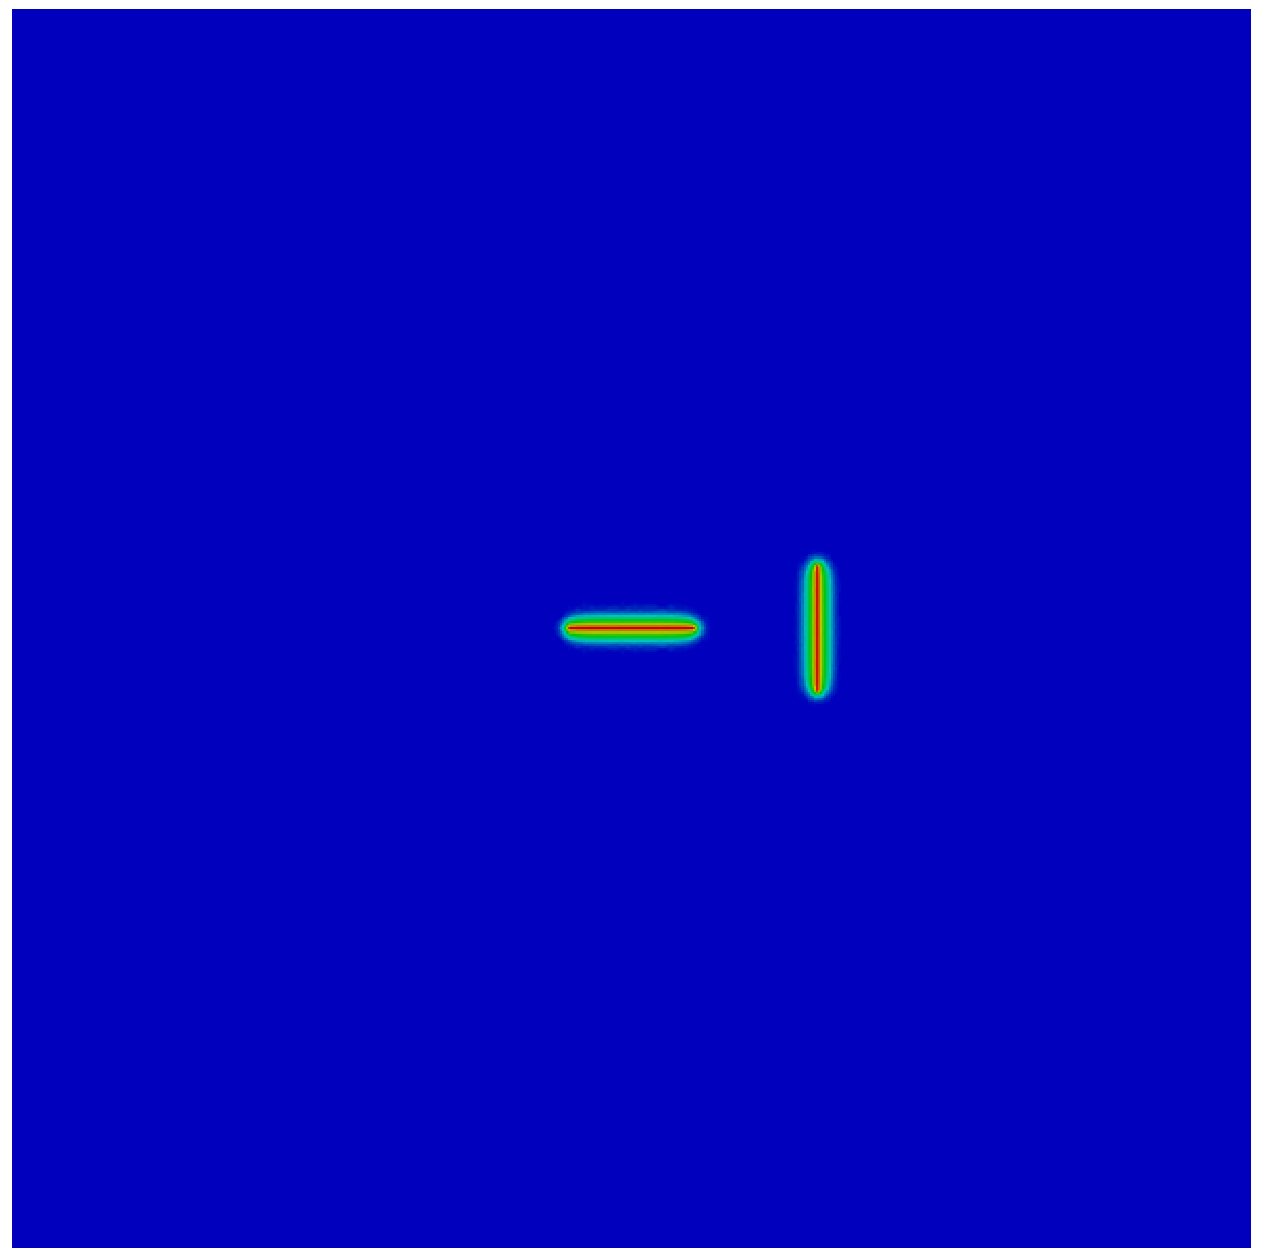
\includegraphics[width=65mm]{alpha_inter_0}\label{Fig:alpha_inter_0}}
\subfloat[]{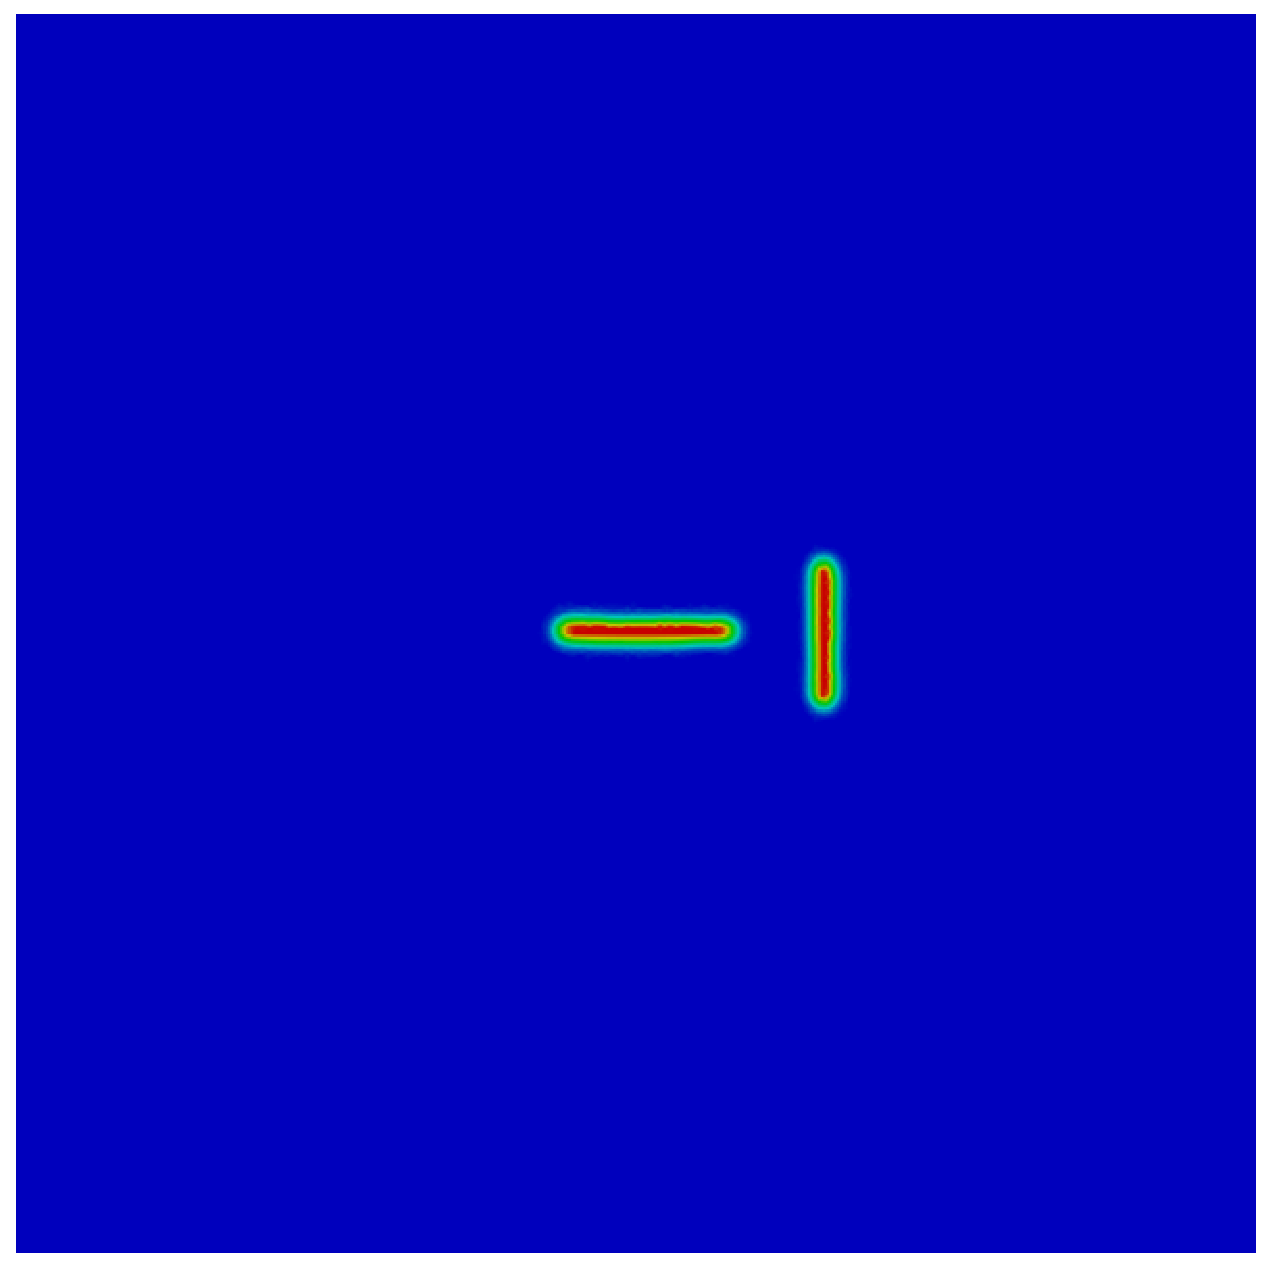
\includegraphics[width=65mm]{alpha_inter_112}\label{Fig:alpha_inter_112}}
\\
\subfloat[]{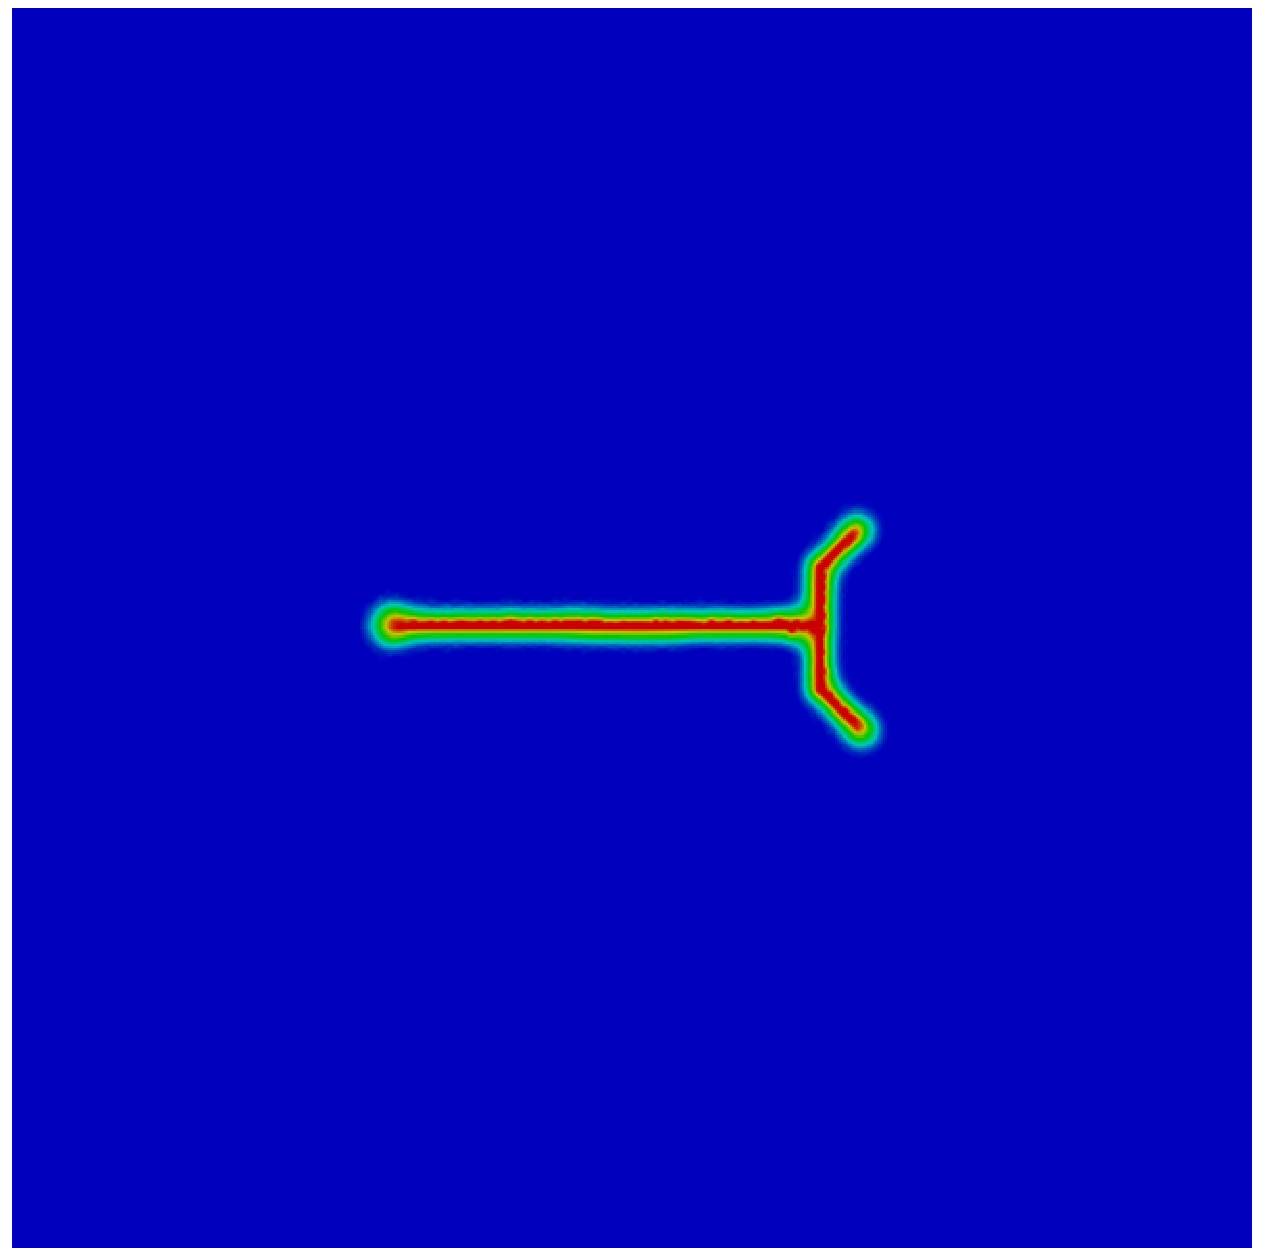
\includegraphics[width=65mm]{alpha_inter_113}\label{Fig:alpha_inter_113}}
\subfloat[]{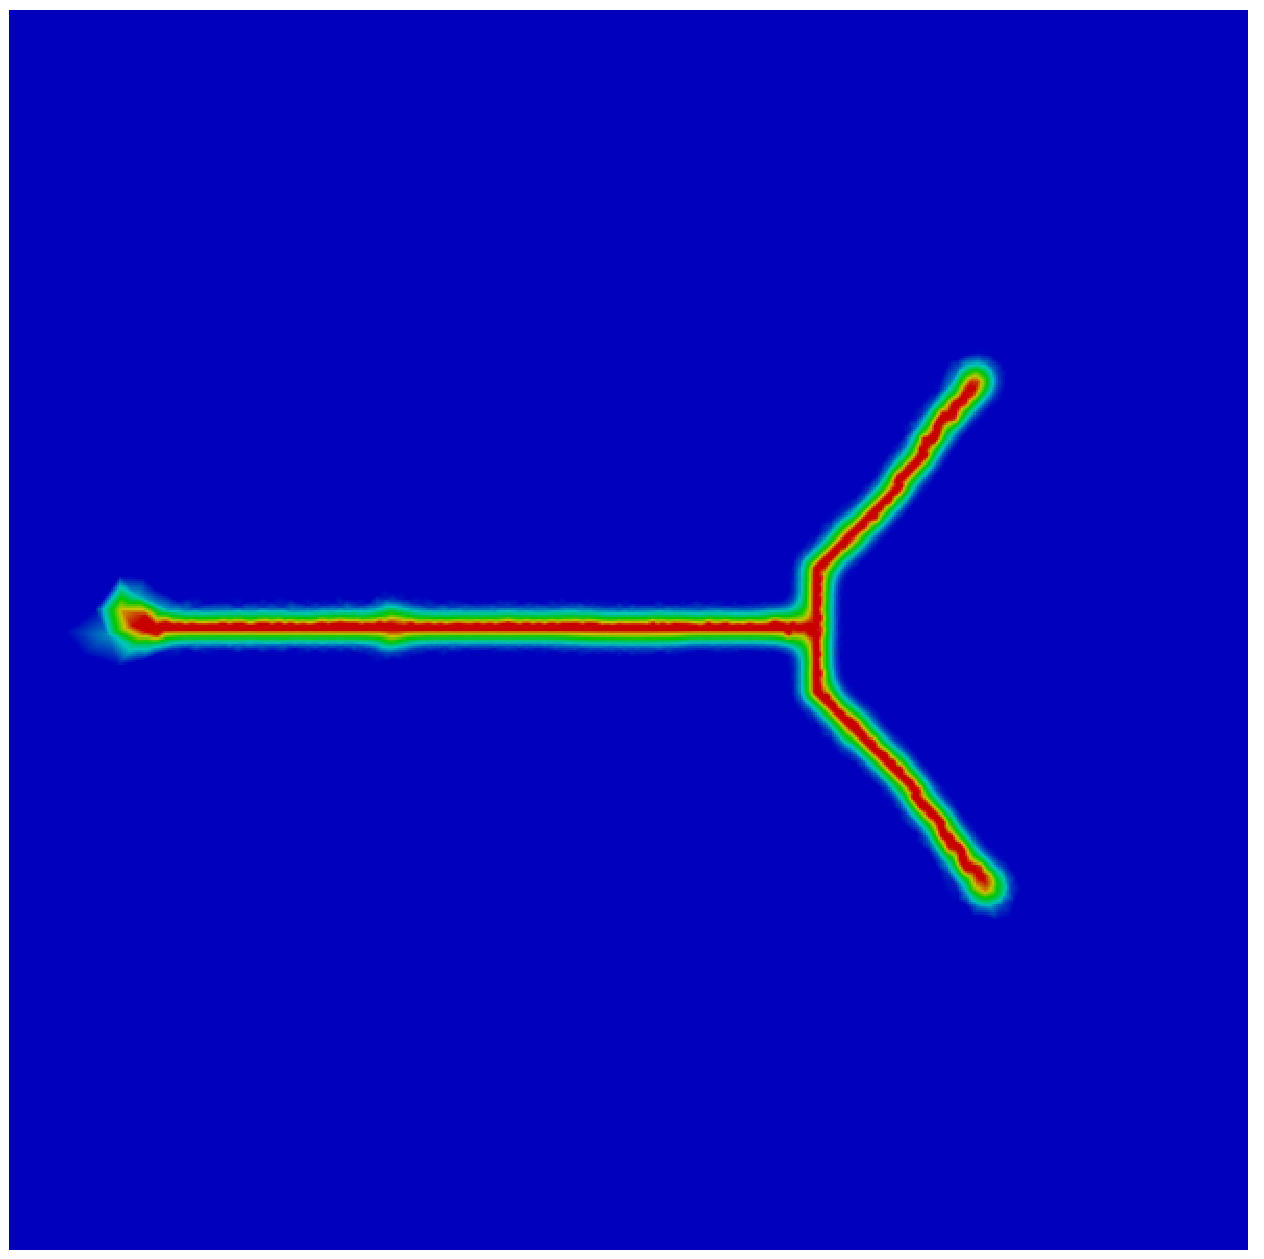
\includegraphics[width=65mm]{alpha_inter_114}\label{Fig:alpha_inter_114}}\\
\subfloat{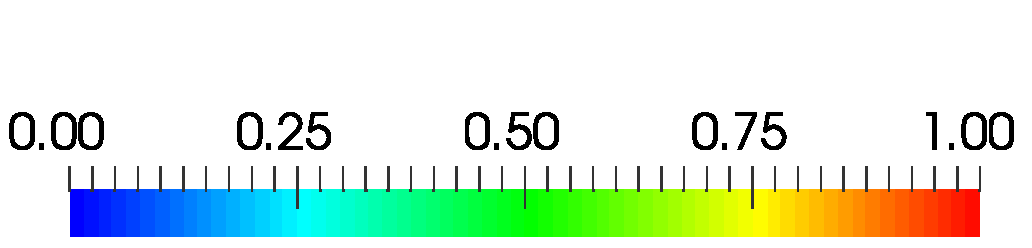
\includegraphics[width=80mm]{alpha_inter_COLORBAR}}

\caption{\added{Increasing pressure leading to joining fractures ($p=m\bar{p}$). Phase field contours at different load steps (\ref{Fig:alpha_inter_0}) $m=1$, (\ref{Fig:alpha_inter_112}) $m=113$, (\ref{Fig:alpha_inter_113}) $m=114$, and (\ref{Fig:alpha_inter_114}) $m=115$. The results show that the horizontal fracture  starts to propagate at $m=113$, and at $m=114$ it intesects the vertical fracture.}}
\label{Fig:Alpha_pressurized_interaction_snapshots}
\end{figure}

\subsection{\added{CO$_2$-driven fracture}} \label{sec: co2_propagation_ex}
In this example, we investigate the fracture propagation in a square plate with a pressurized CO$_2$ flow, with \cite{ishida2016features, wang2018influence} as the benchmarks. The specimen has edge lengths of $L=170$ mm. The geometric setup and boundary conditions are depicted in Figure \ref{Fig:Gas_geometry}. The sample is discretized into 4,832 three-noded triangular elements so that the mesh size $h\approx 5.68$ mm is obtained. Also, we set $\ell=1.6$ mm. Table \ref{Tab:Gas_input} shows the remaining parameters to be input.

\begin{figure}[htbp]
	\centering
	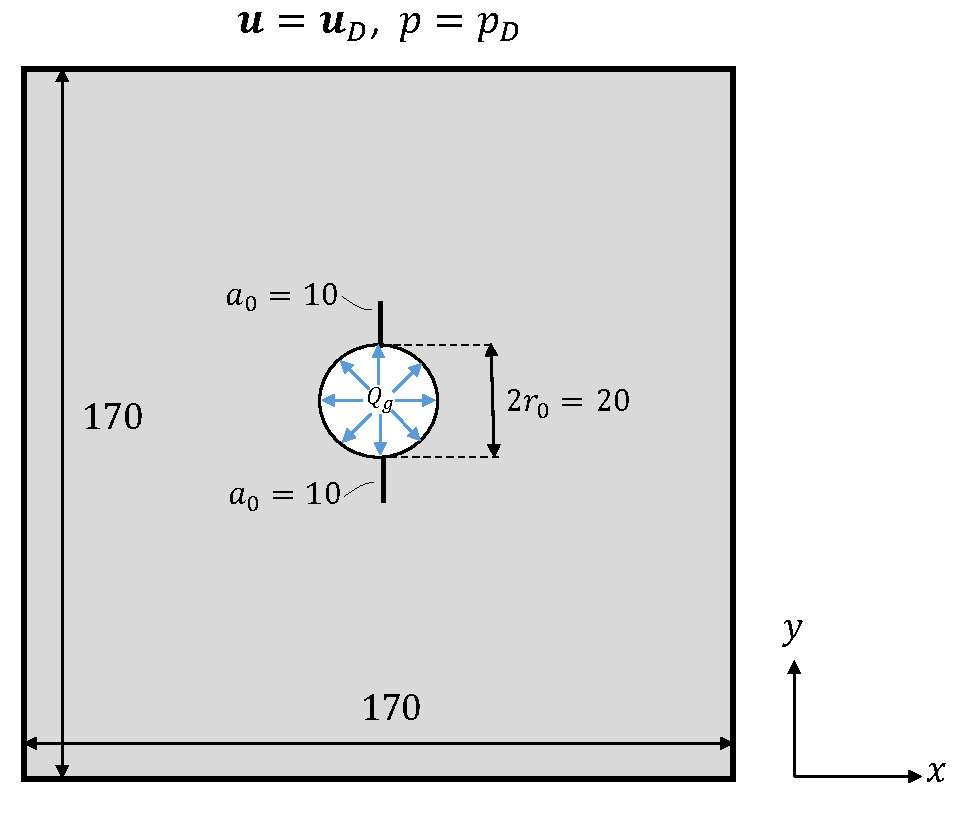
\includegraphics[width=0.8\textwidth]{GasFrackingModel2}
	\caption{Schematic of a fractureed square plate (unit: mm) with pressurized CO$_2$ flow.}
	\label{Fig:Gas_geometry}
\end{figure}

As in Figure \ref{Fig:Gas_geometry}, there exist two preexisting fractures representing the perforations. We set $d=1$ for both fractures and set the Dirichlet boundary condition $d=0$ on the external boundary. The fluid is continuously injected into the central borehole with diameter $2r_0=20$ mm, until after the fractures propagate. Note that in this problem, the isothermal condition is adopted so that CO$_2$ is in the supercritical phase ($T=45^{\circ}$C).
%\todo[inline]{We have to mention our computation domain would be $\Omega-$ the borehole. It  is worth to mention the boundary of borehole is denoted by $\gamma_B$\\Vahid: Now that we have added Figure \ref{Fig:compute_domain}, there is no need for further explanations here.}

For the sake of simplicity, the \emph{in situ} stress \added{$\sigma_1=\sigma_3=1$ MPa} is imposed on the boundary by means of its ``equivalent'' prescribed displacement. More precisely, the displacement of the same specimen with no fracture under the same \emph{in situ} stress is first computed, then used as the Dirichlet boundary condition for the problem at hand. On the external boundary, we set $p=p_D$ where $p_D=0$. Moreover, $\Gamma_P=\Gamma_D$ in this example.

%\todo[inline]{YS: What is the purpose of putting a reference \cite{wang2018influence} ALONE in the title of Table \ref{Tab:Gas_input}? More words are needed, like ``according to.''\\Vahid: Changed.}

\begin{table}[htbp]
    \centering
    \caption{Default parameter values for the example. These values are taken from \cite{wang2018influence} except $g_c$, which is from \eqref{Eq:choice_ell}.}

    \begin{tabular}{l c c c}
    \hline 
         Parameters & symbol & unit& value \\
    \hline 
         Young's modulus & $E$ &MPa&  6 $\times 10^{3}$\\
         Poisson's ratio & $\nu$ &$-$&  0.34\\
         Critical energy release rate & $g_c$ &MPa$\cdot$mm&  0.306\\
         %Regularization length scale & $\ell$ &$-$&  1.6$\times 10^{-4}$\\
         Biot coefficient & $\alpha$ &$-$&  0.85\\
         Porosity & $\phi$ &$-$&  0.01\\
         Initial permeability & $k_0$ &mm$^2$&  1$\times 10^{-12}$\\
         Dynamic viscosity of {CO}$_2$ & $\mu$ & MPa$\cdot$s& 4.04$\times 10^{-11}$\\
         %Bulk modulus of fluid & $k_f$ &$KN/mm^2$&  0.625$ \times 10^{3}$\\
        % Bulk modulus of rock & $k_s$ &$KN/mm^2$&  10$ \times 10^{3}$\\
         Initial pressure & $p_0$ &MPa& 0.1\\
         Rock's tensile strength & $\sigma_T$ &MPa& 11\\
         %Maximum principal stress & $\sigma_1$ &MPa&  1\\
         %Minimum  principal stress & $\sigma_3$ &MPa&  1\\

    \hline     
    \end{tabular}
    \label{Tab:Gas_input}
\end{table}

%\begin{figure}[htbp]
%\centering %
%\subfloat[]{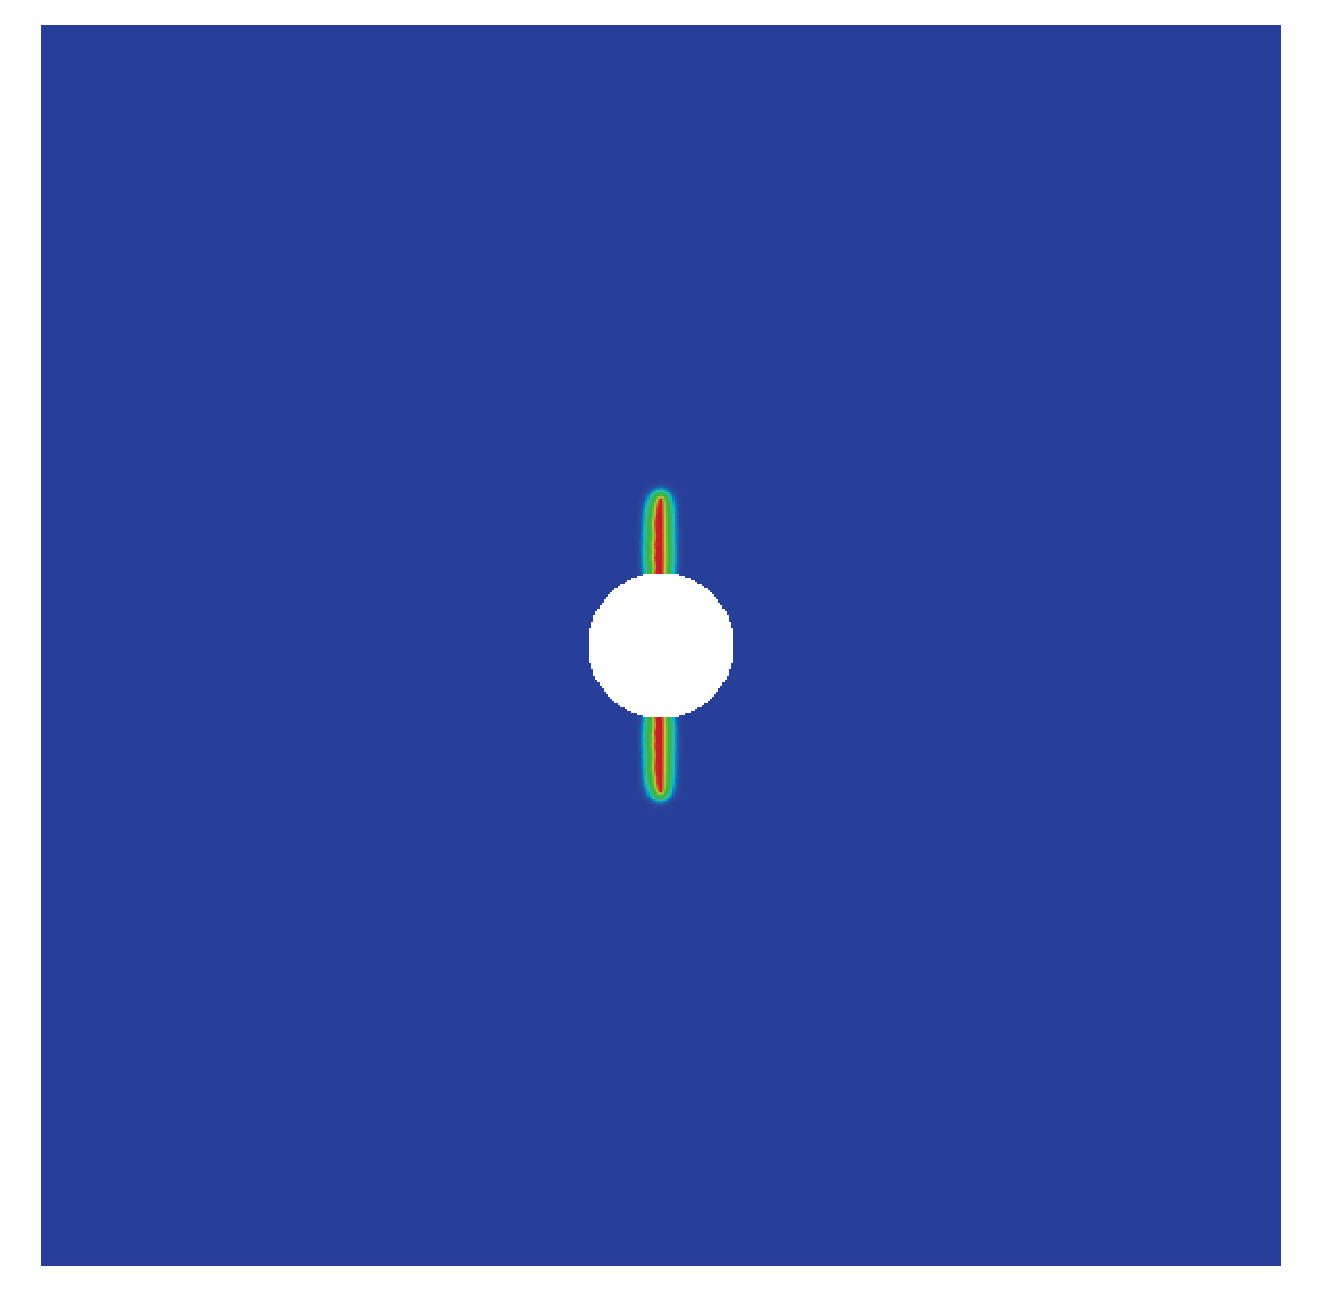
\includegraphics[width=60mm]{alpha_50.eps}\label{Fig:Gas_d_i}}
%\subfloat[]{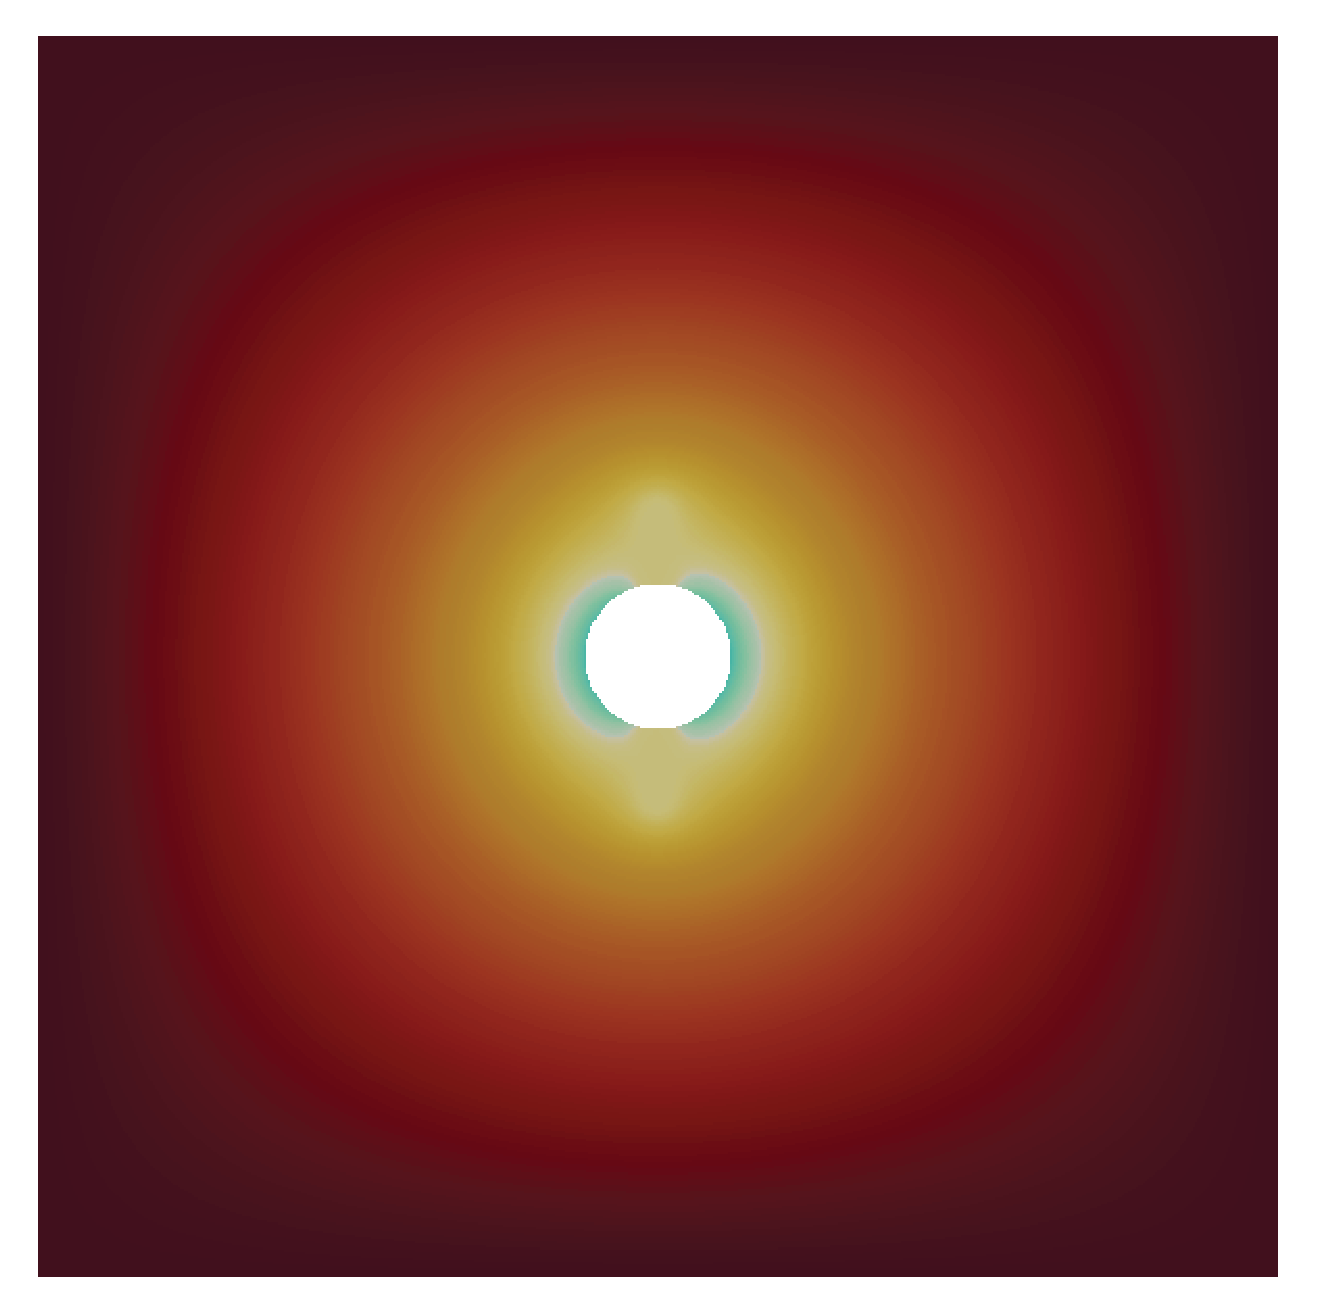
\includegraphics[width=60mm]{pressure_50.eps}\label{Fig:Gas_p_i}}\\
%\subfloat[]{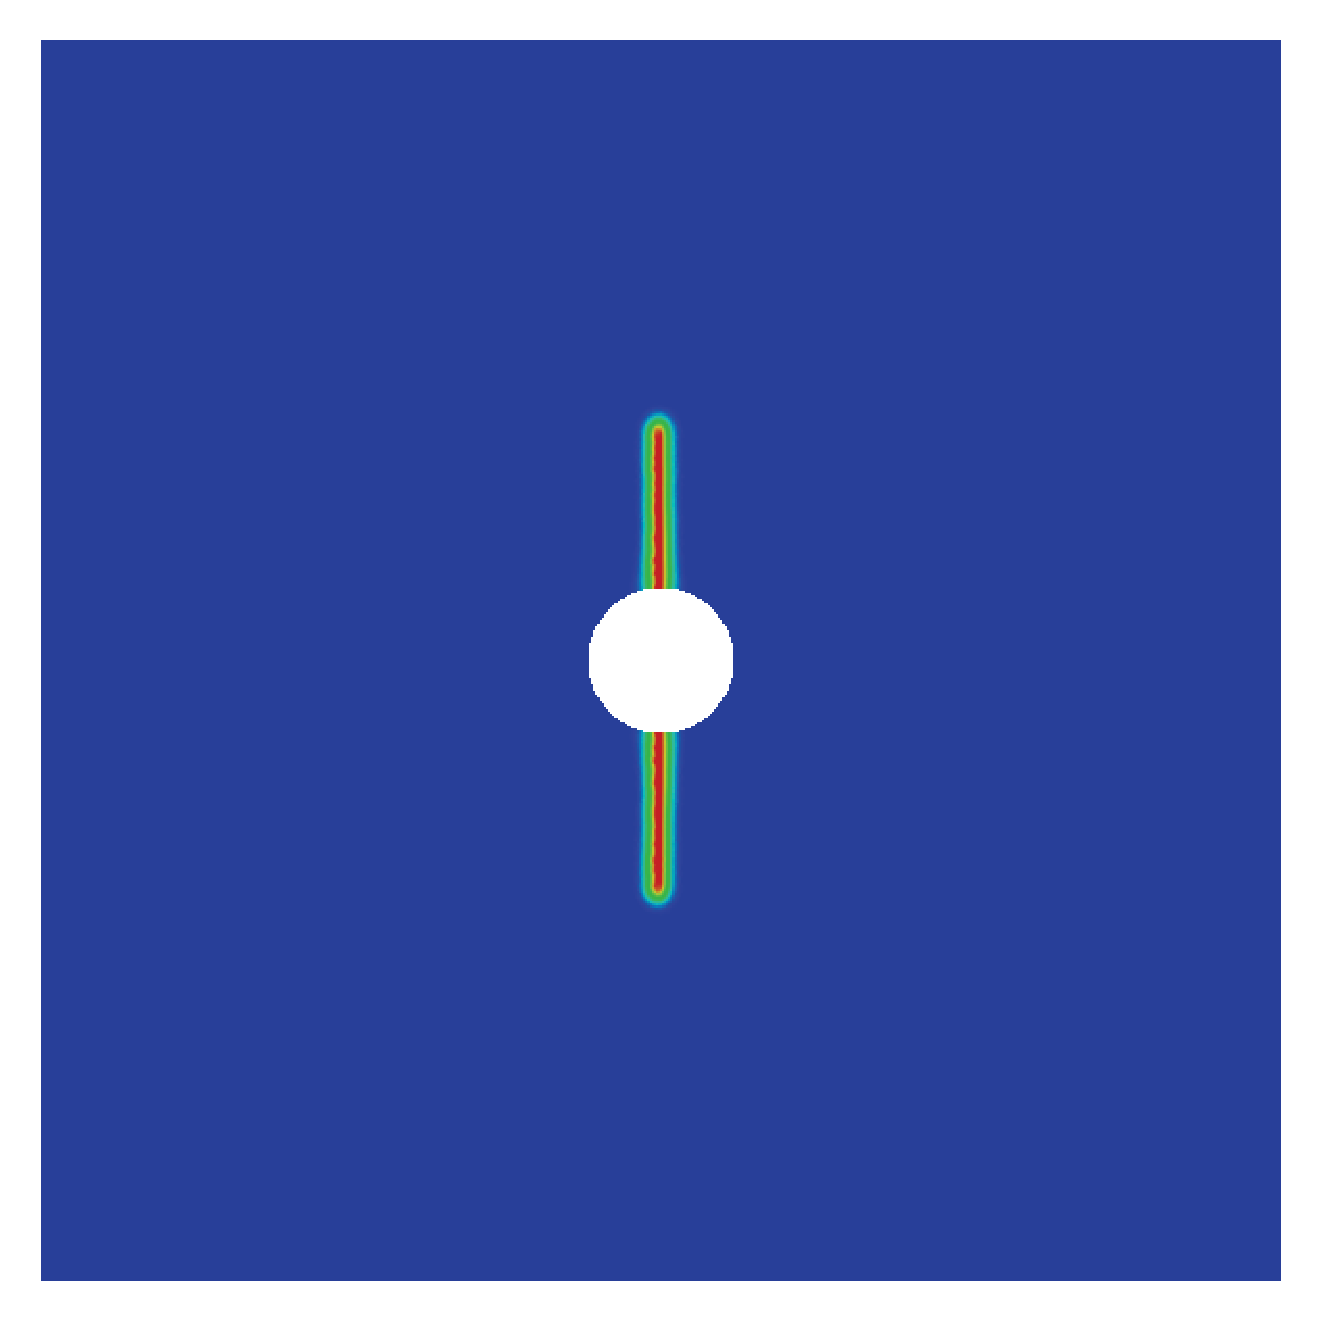
\includegraphics[width=60mm]{alpha_75.eps}\label{Fig:Gas_d_ii}}
%\subfloat[]{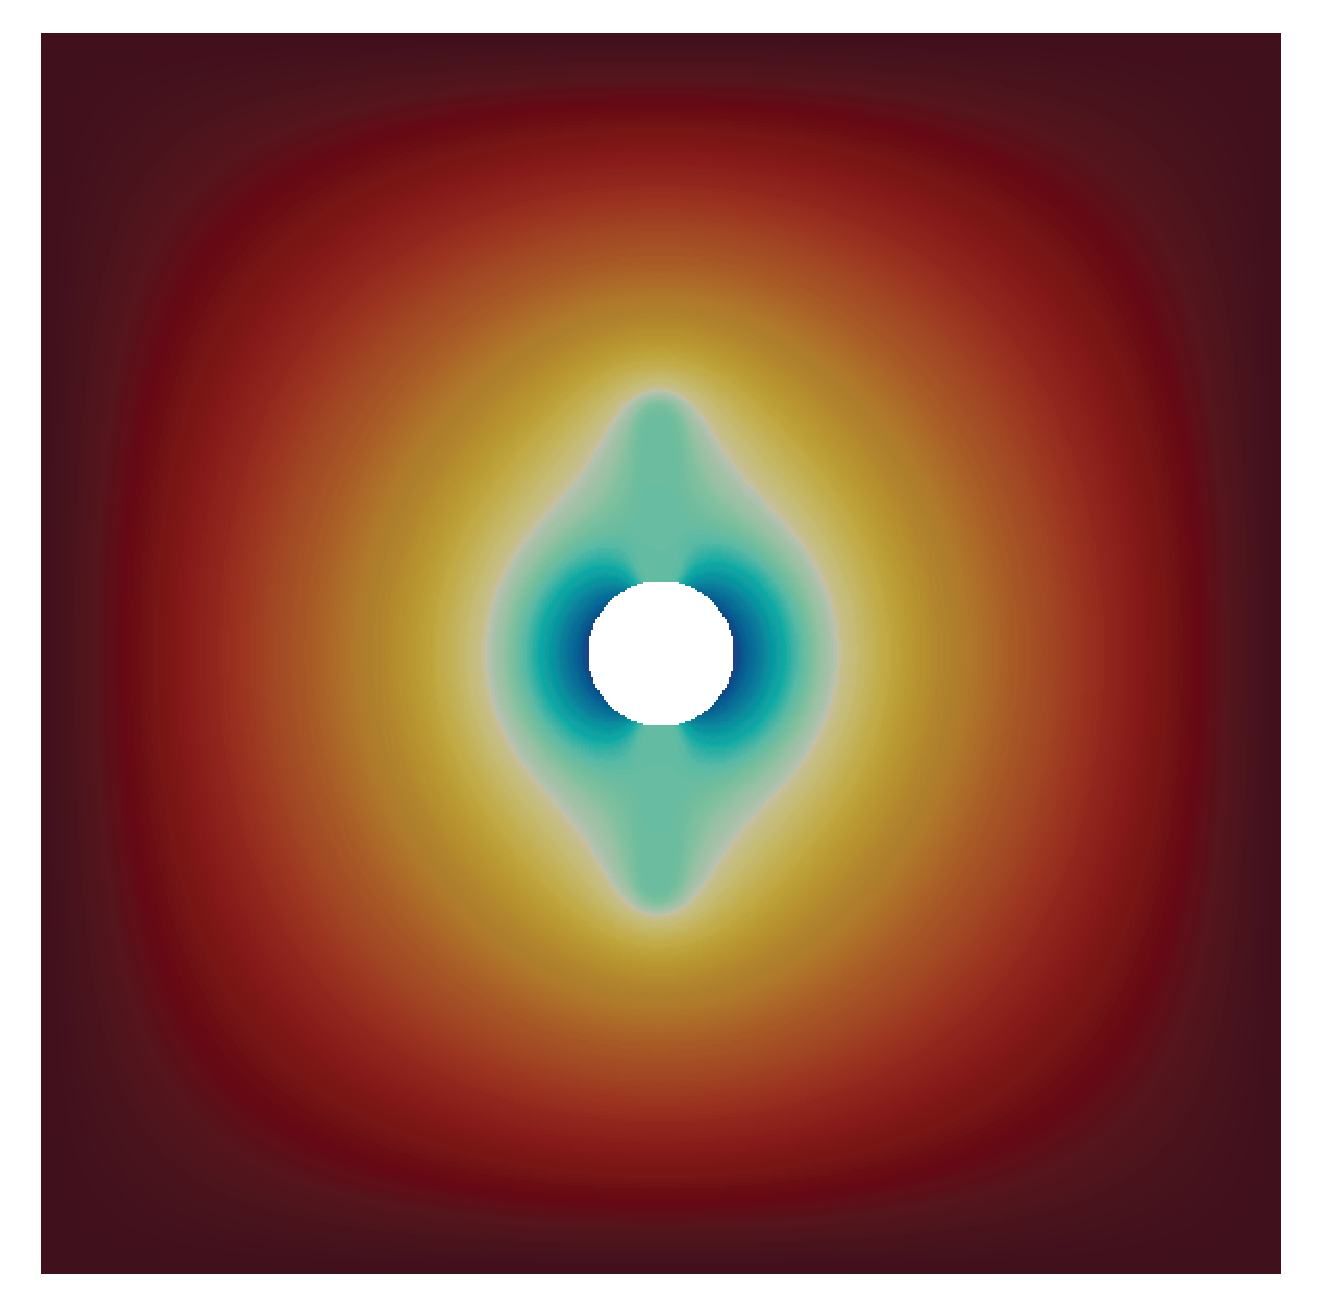
\includegraphics[width=60mm]{pressure_75.eps}\label{Fig:Gas_p_ii}}\\
%\subfloat[]{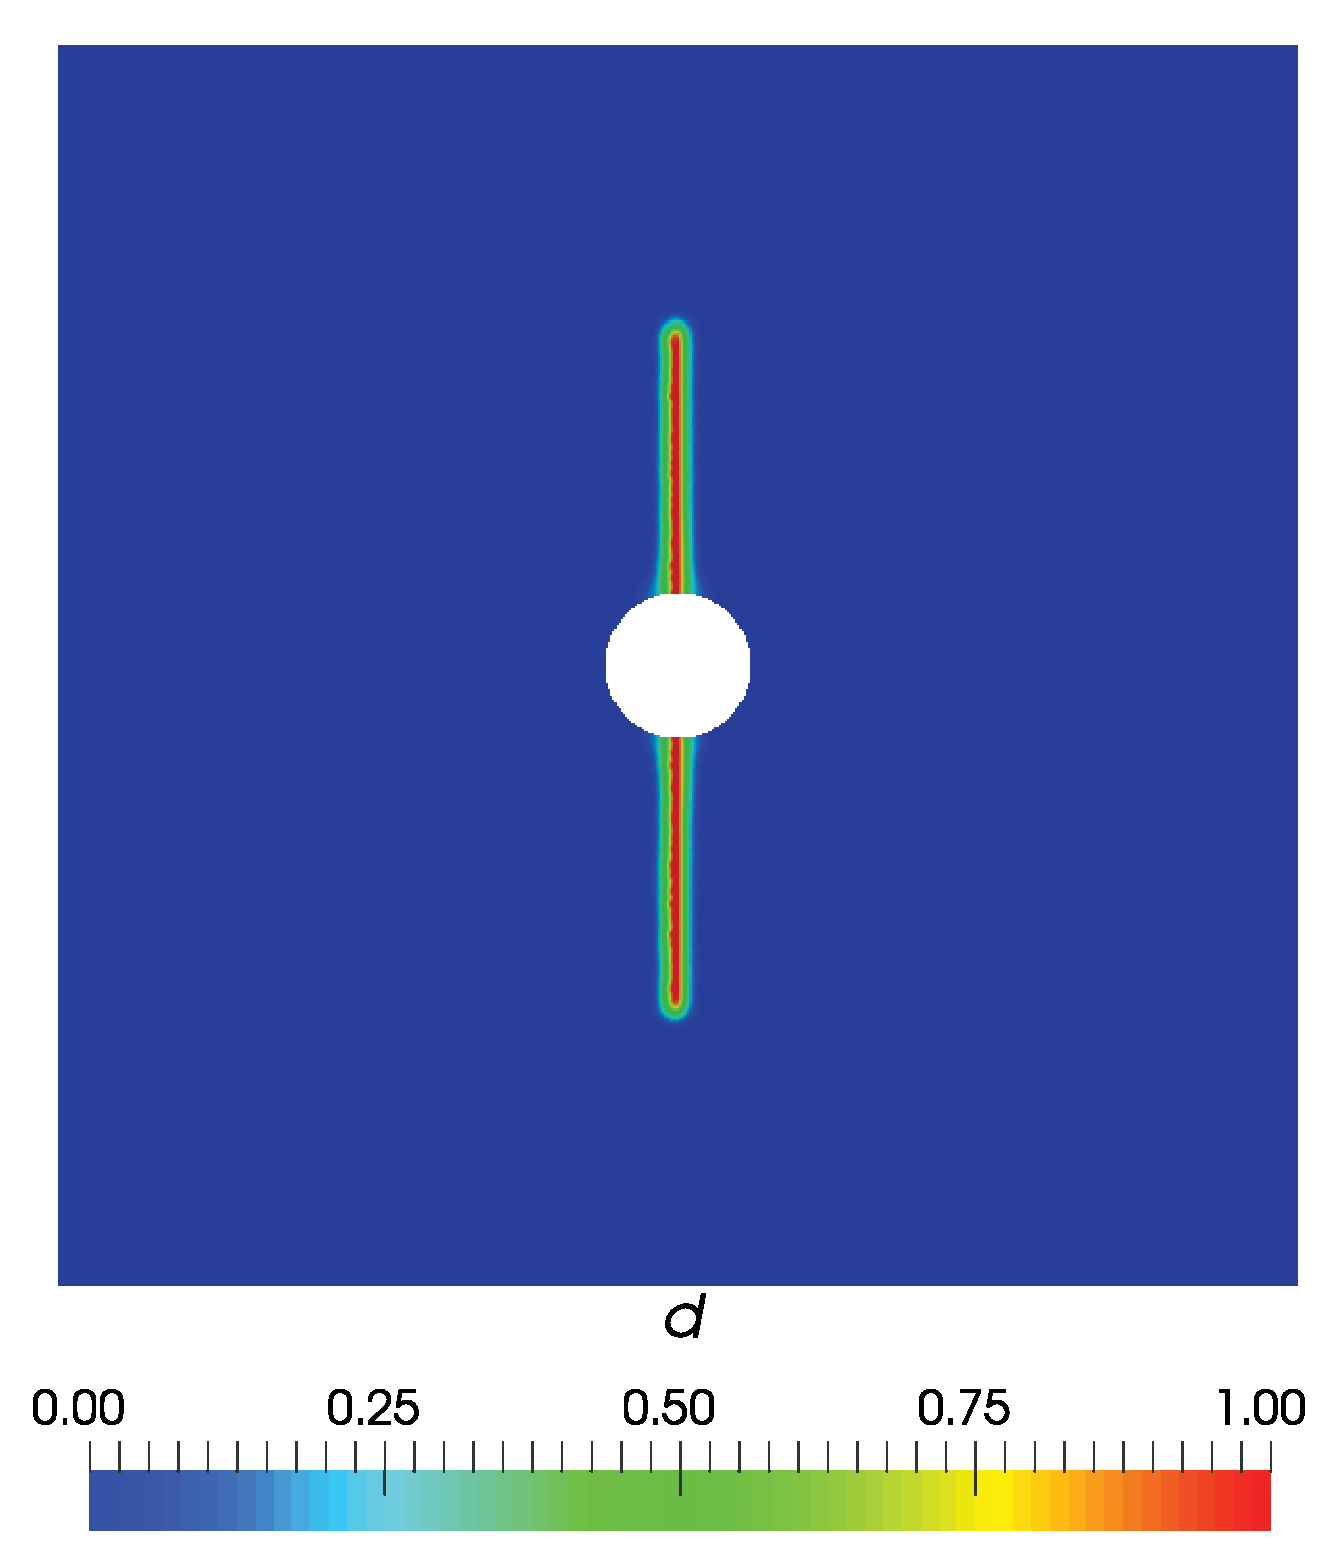
\includegraphics[width=60mm]{alpha_100.eps}\label{Fig:Gas_d_iii}}
%\subfloat[]{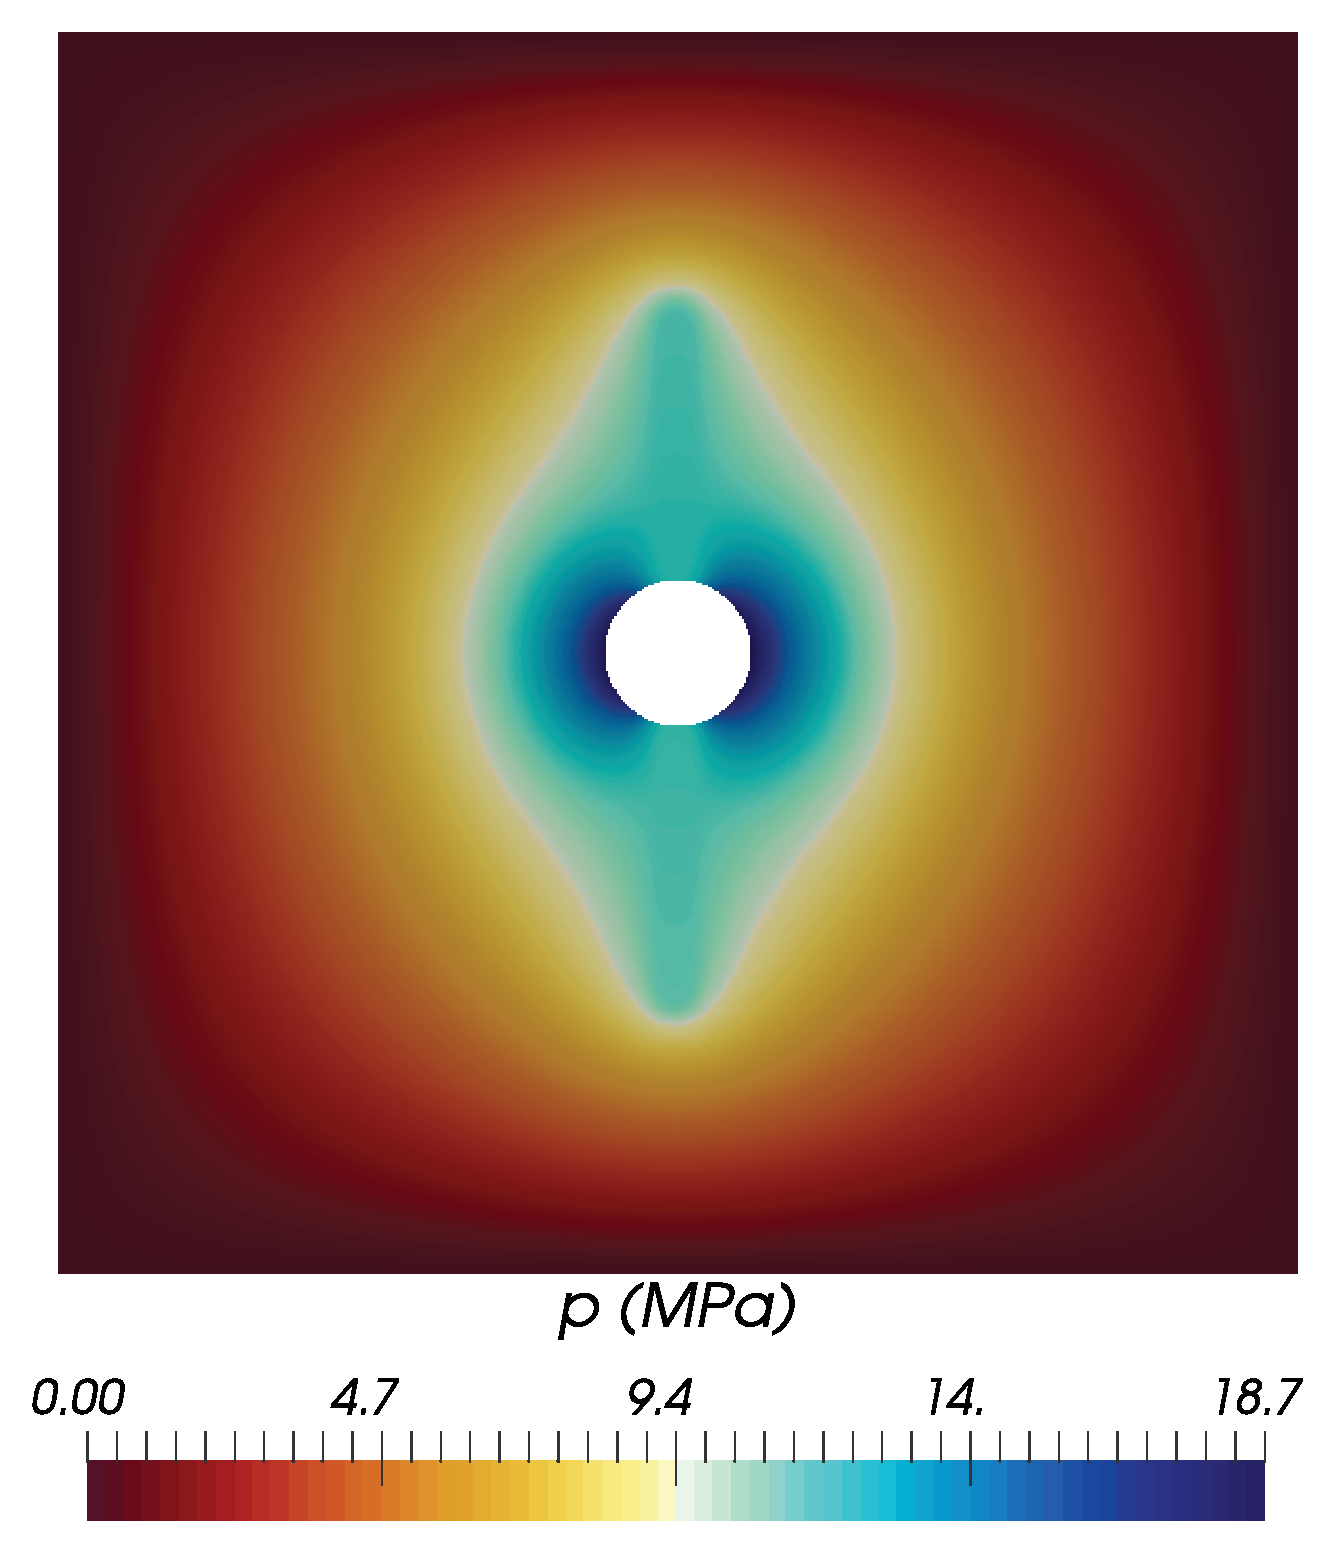
\includegraphics[width=60mm]{pressure_100.eps}\label{Fig:Gas_p_iii}}
%\caption{Left: Phase field diagram at different stages (\ref{Fig:Gas_d_i}) $t=0.5t_f$, (\ref{Fig:Gas_d_ii}) $t=0.75t_f$, and (\ref{Fig:Gas_d_iii}) $t=t_f$). Right: Pressure profile at (\ref{Fig:Gas_p_i}) $t=0.5t_f$, (\ref{Fig:Gas_p_ii}) $t=0.75t_f$, and (\ref{Fig:Gas_p_iii}) $t=t_f$.}
%\label{Fig:Gas_snapshots}
%\end{figure}




\begin{figure}[htbp]
\centering %
\subfloat[]{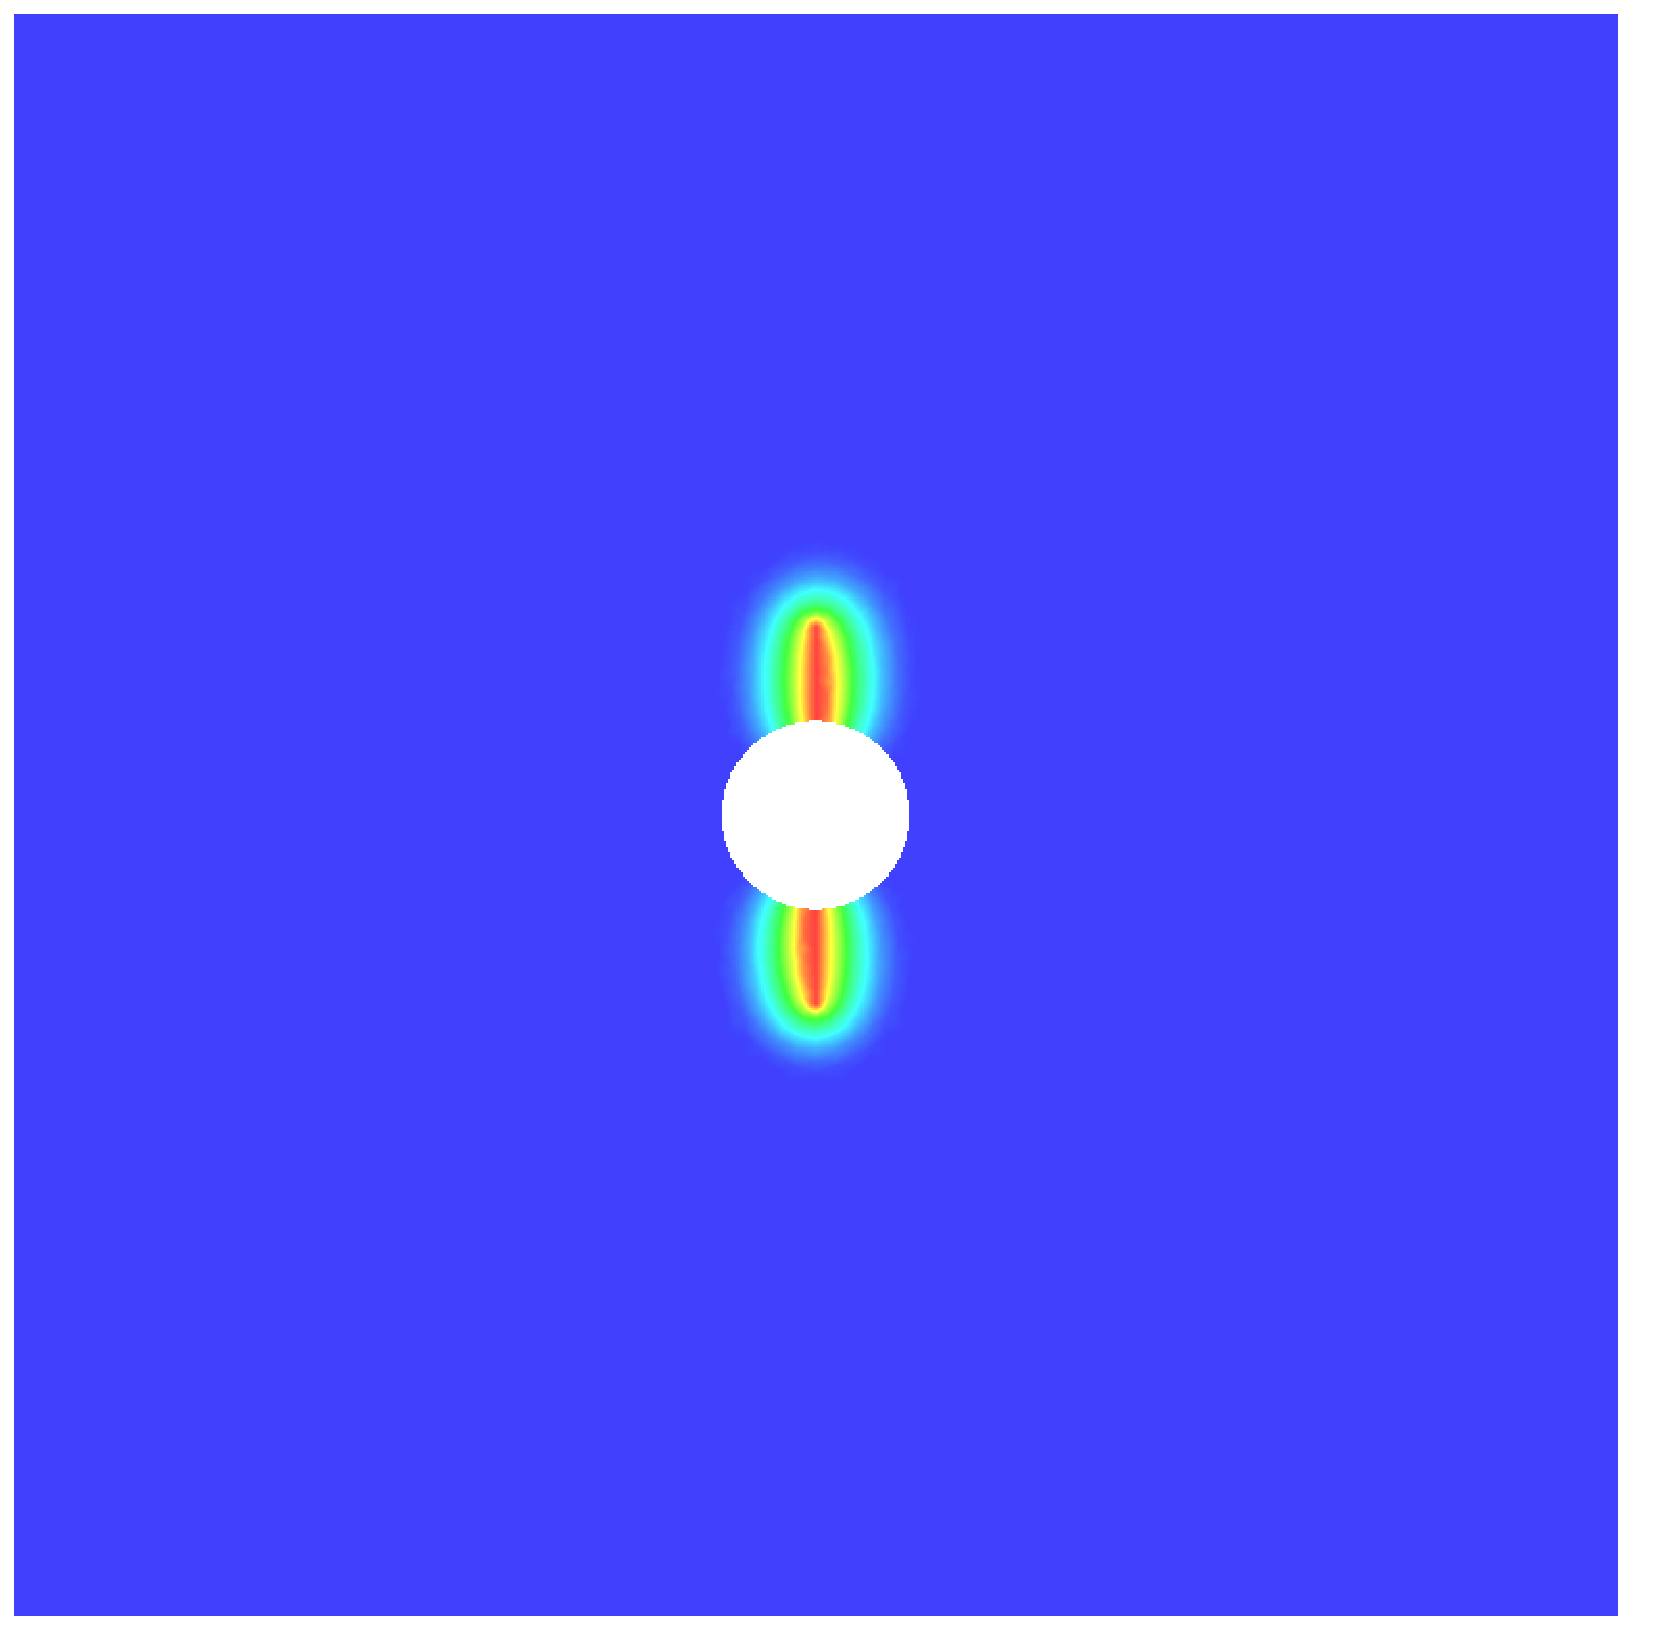
\includegraphics[width=60mm]{alpha25}\label{Fig:Gas_d_i}}
\subfloat[]{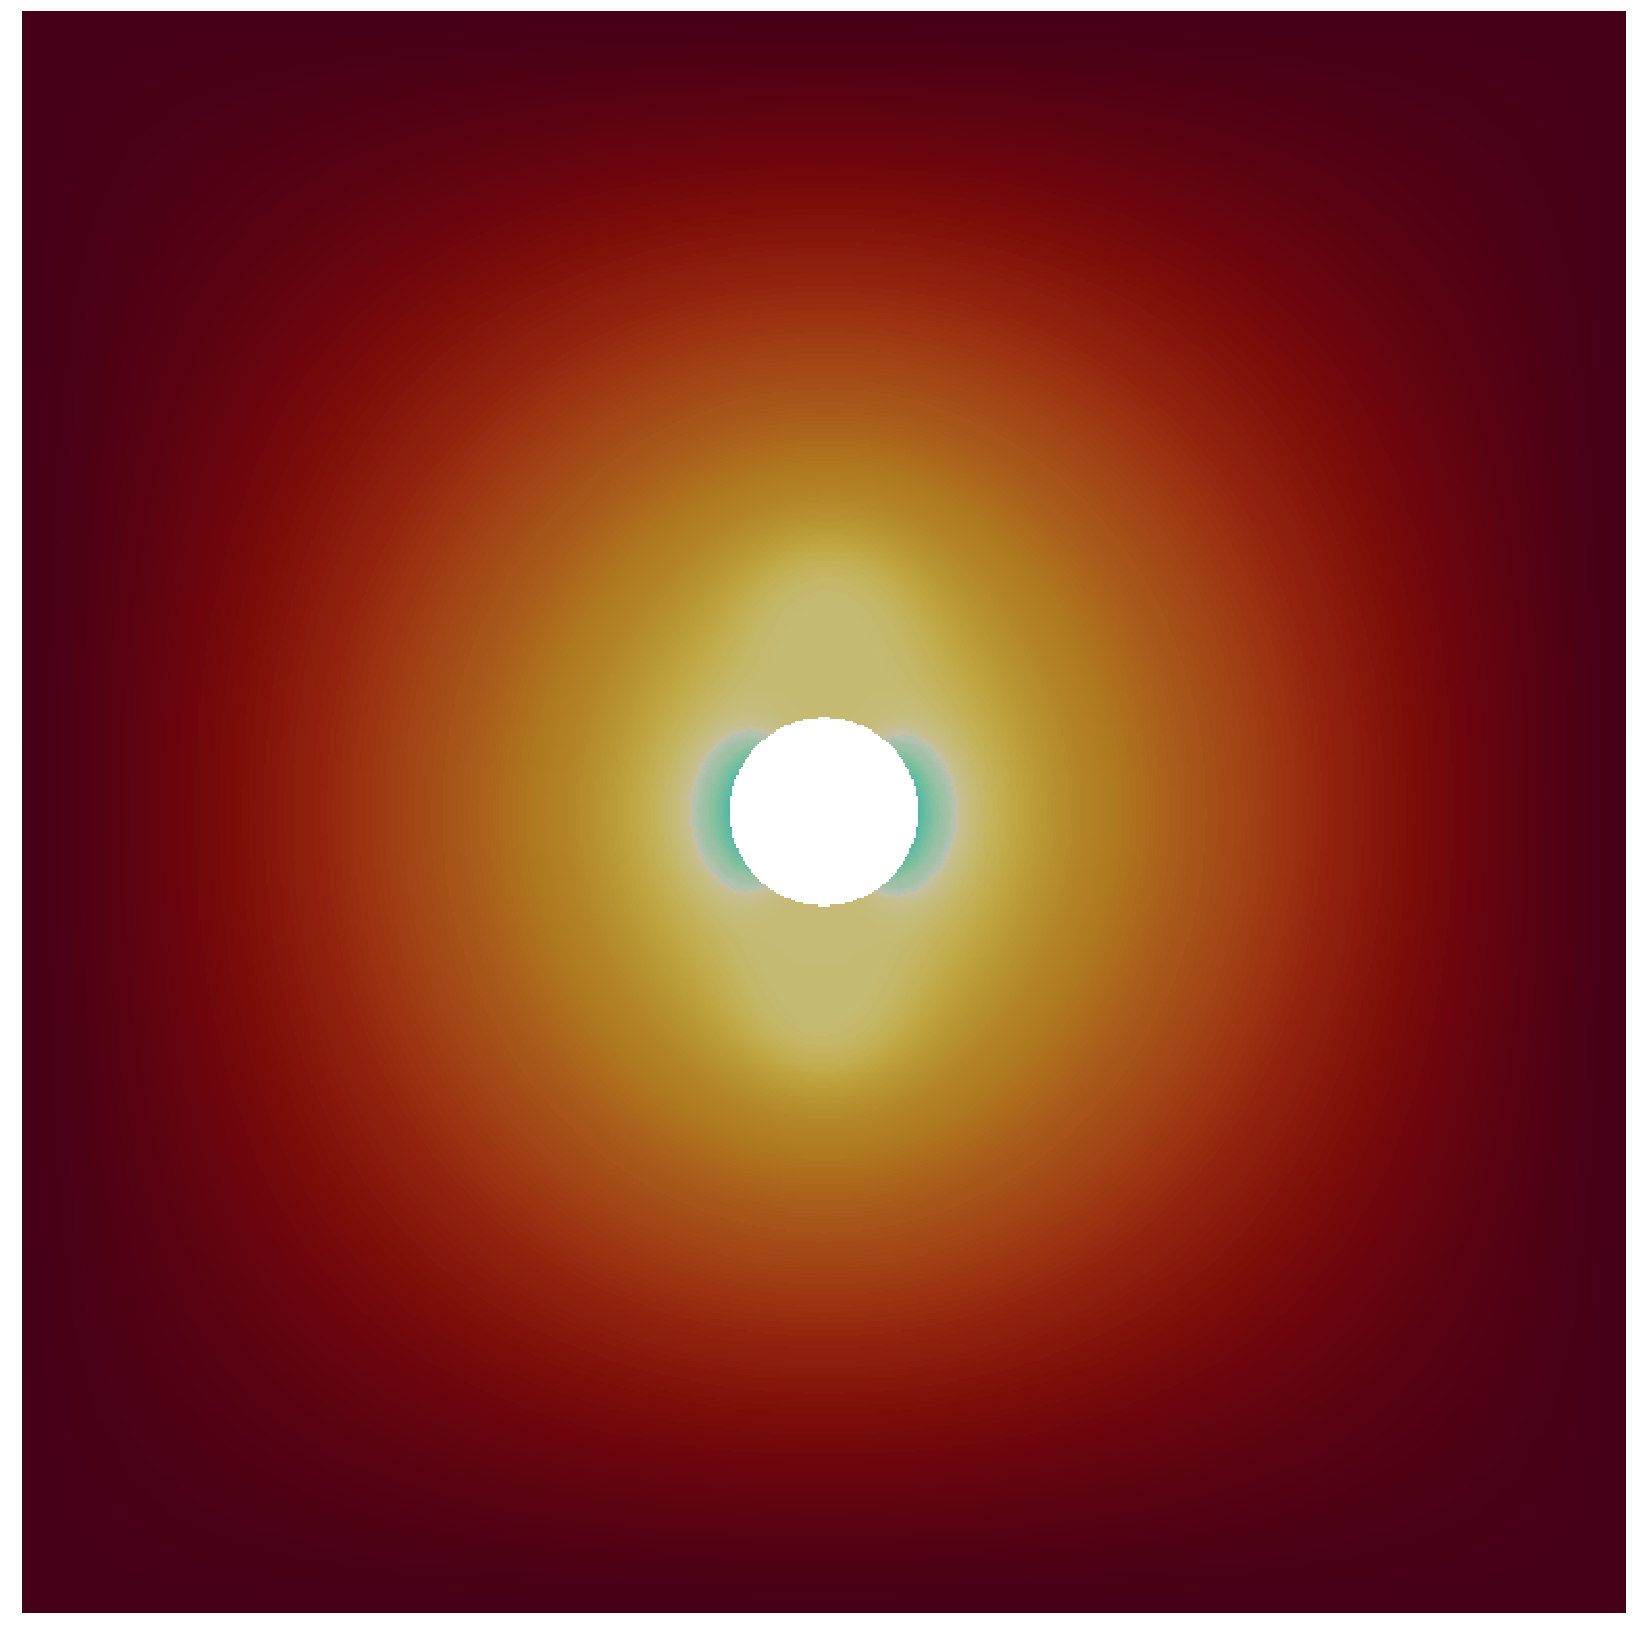
\includegraphics[width=60mm]{pressure25}\label{Fig:Gas_p_i}}\\
\subfloat[]{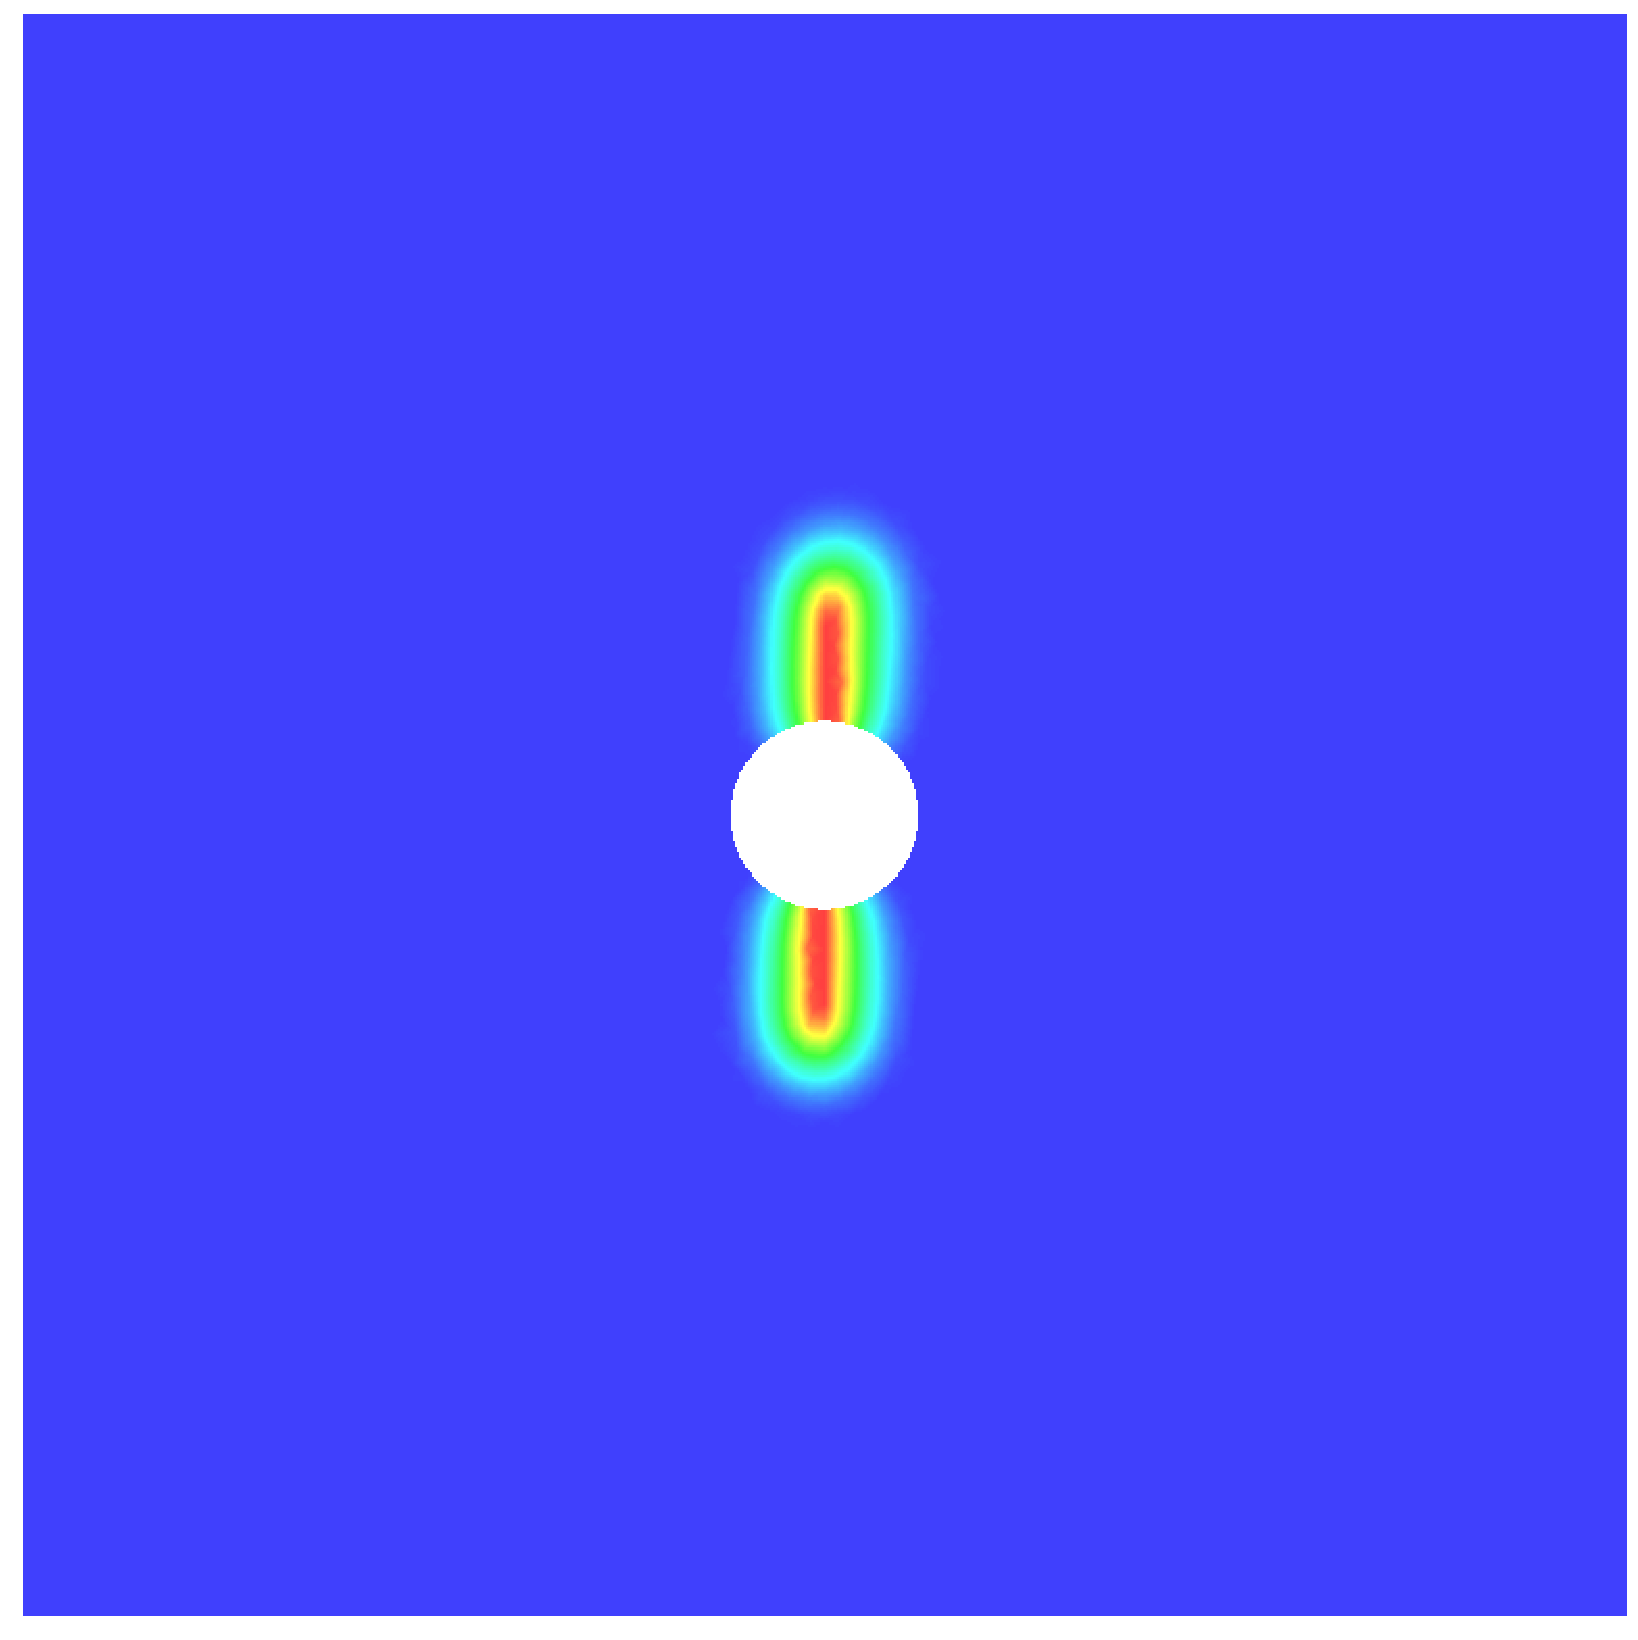
\includegraphics[width=60mm]{alpha37}\label{Fig:Gas_d_ii}}
\subfloat[]{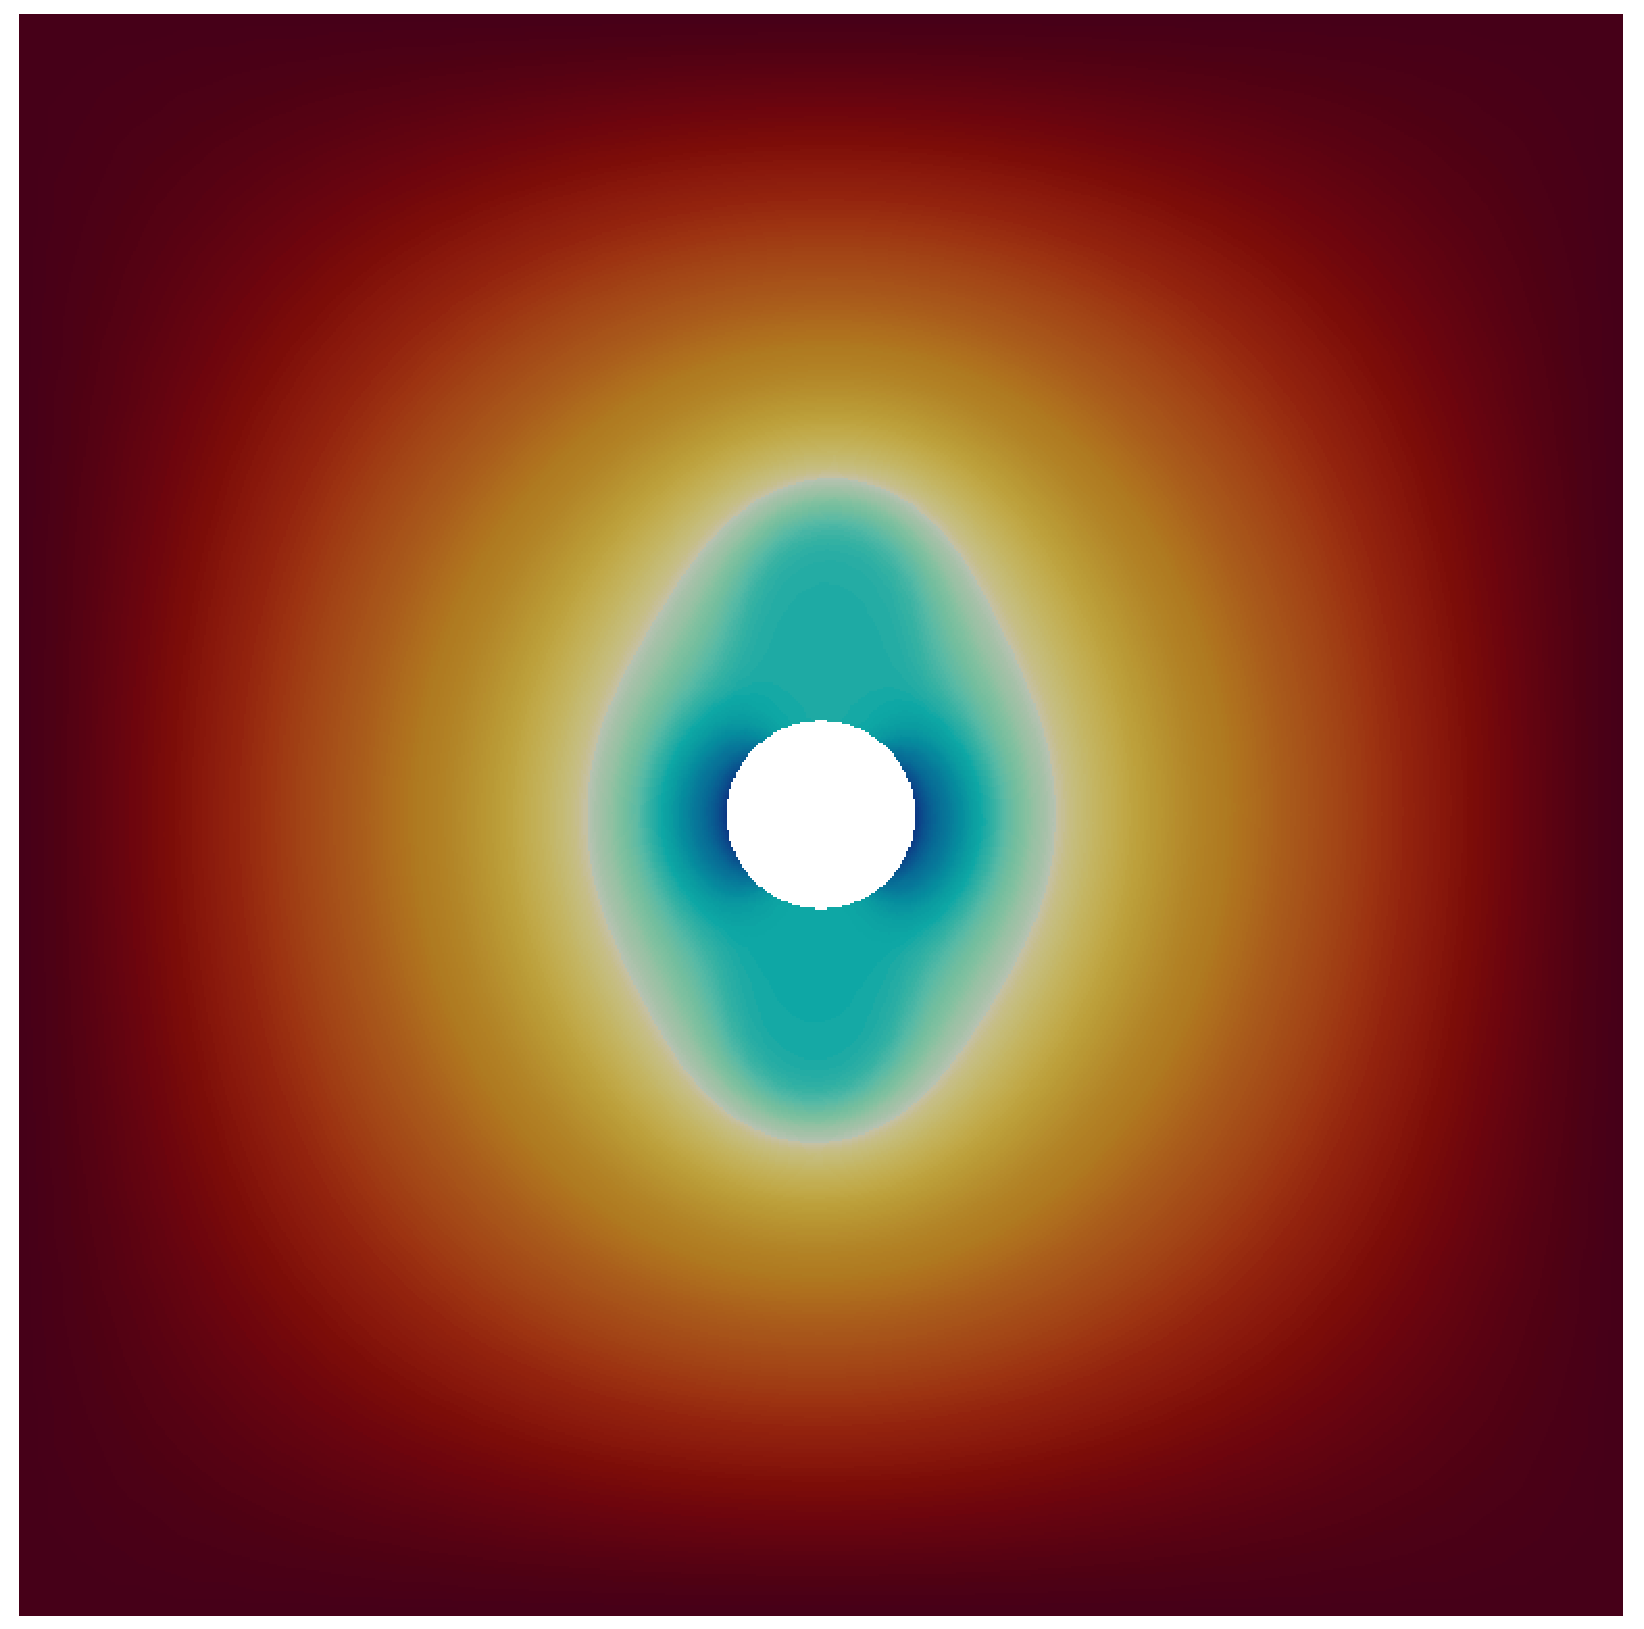
\includegraphics[width=60mm]{pressure37}\label{Fig:Gas_p_ii}}\\
\subfloat[]{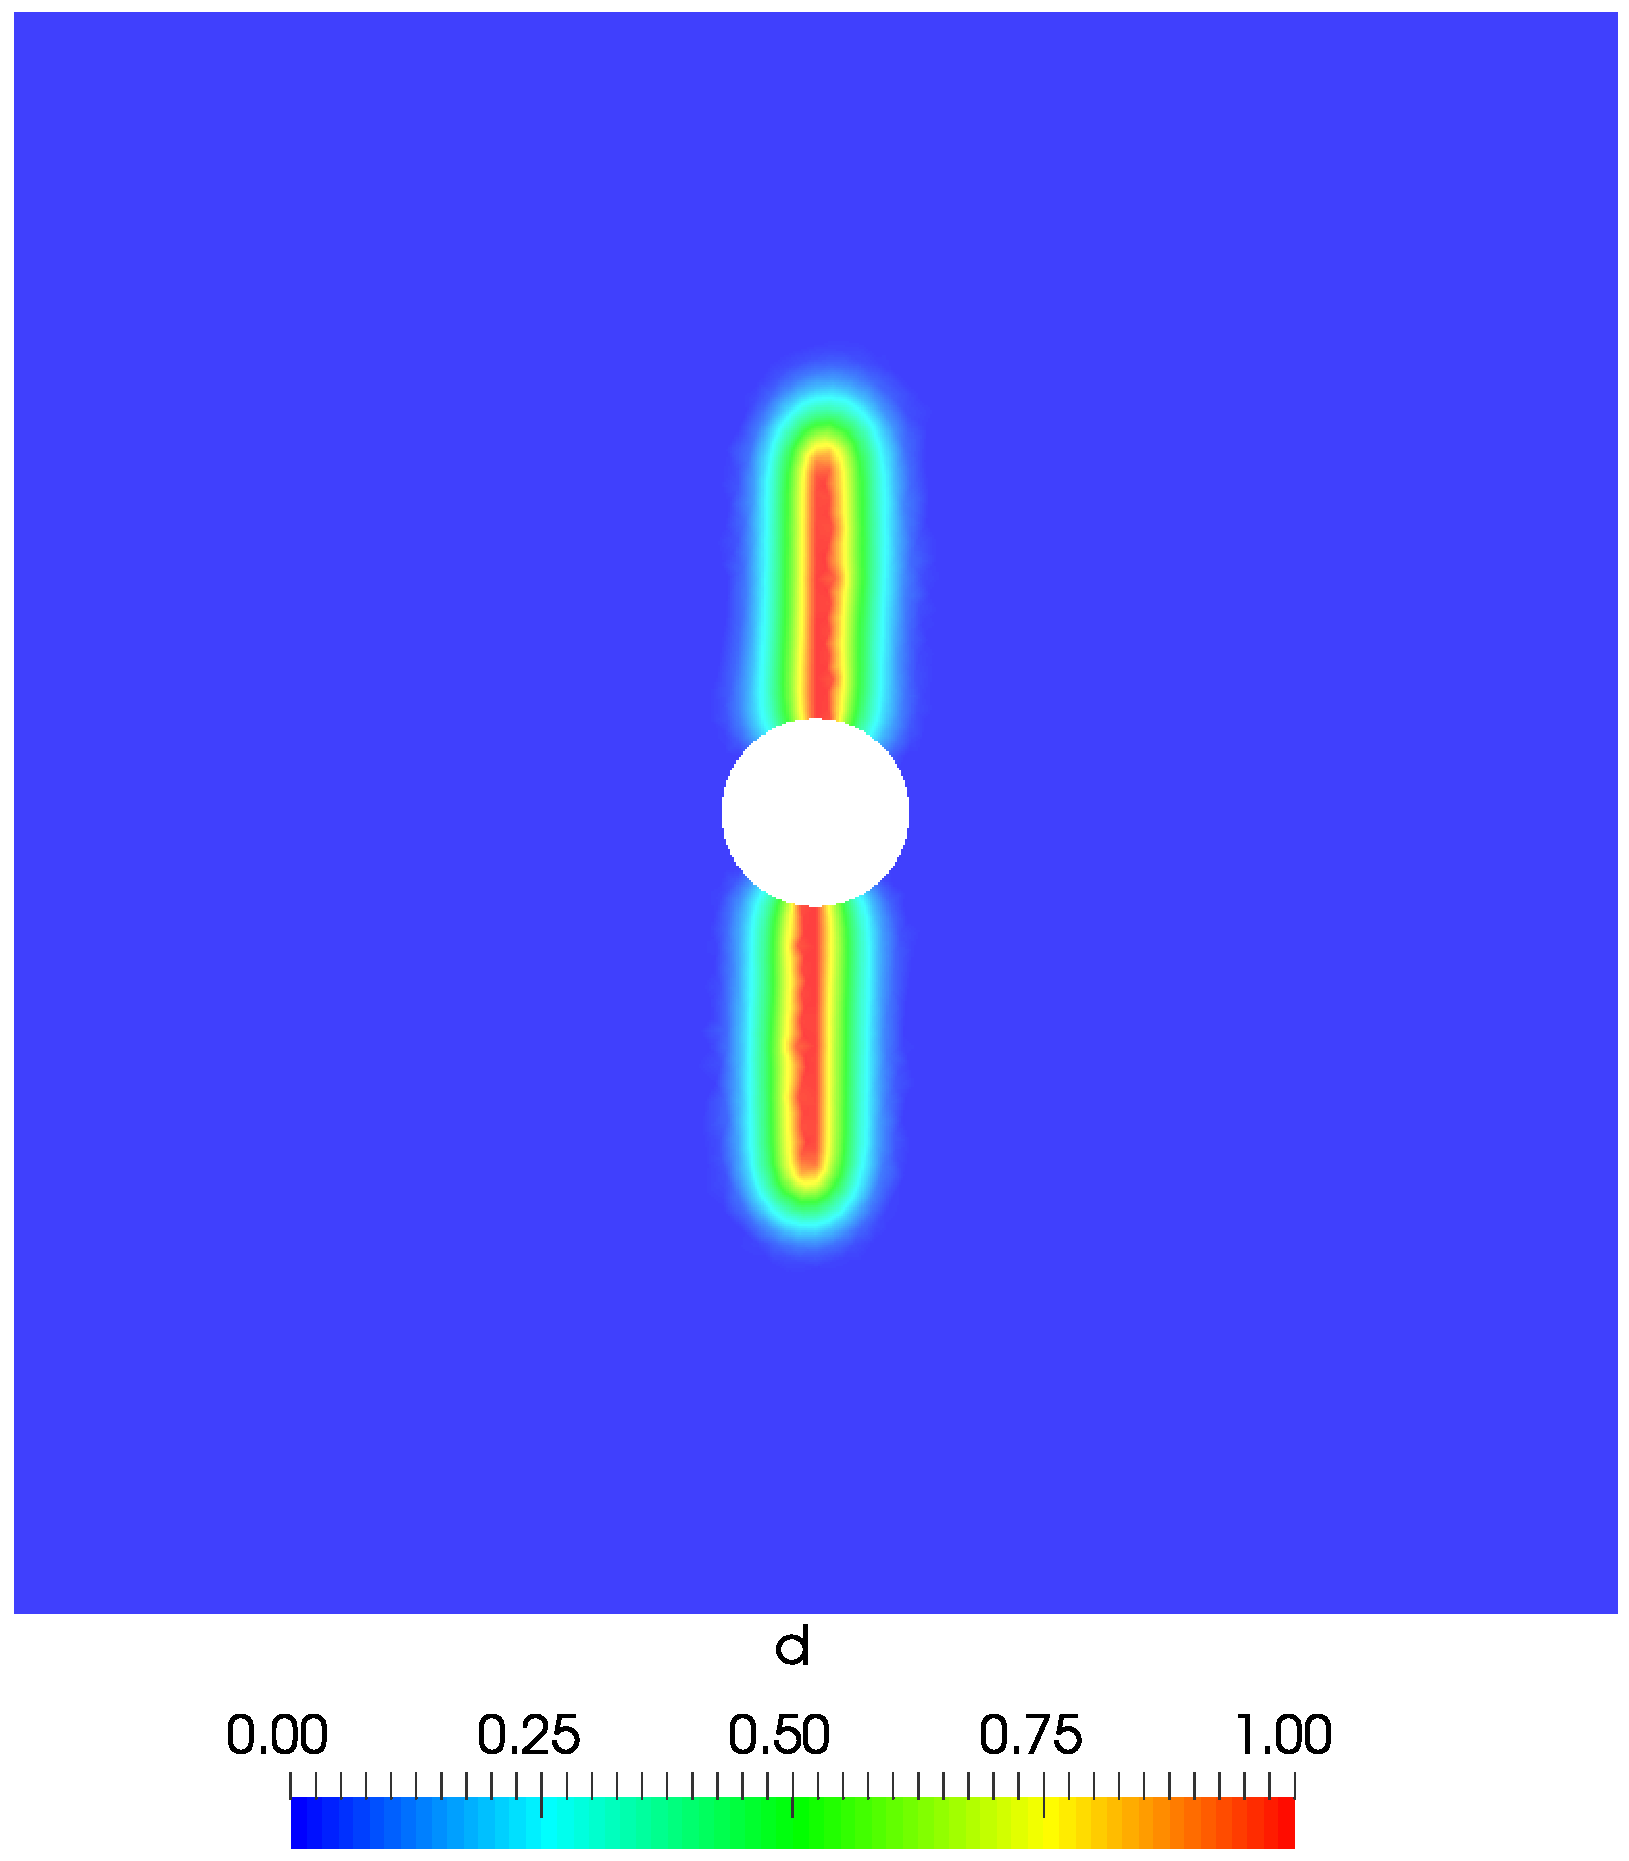
\includegraphics[width=60mm]{alpha49}\label{Fig:Gas_d_iii}}
\subfloat[]{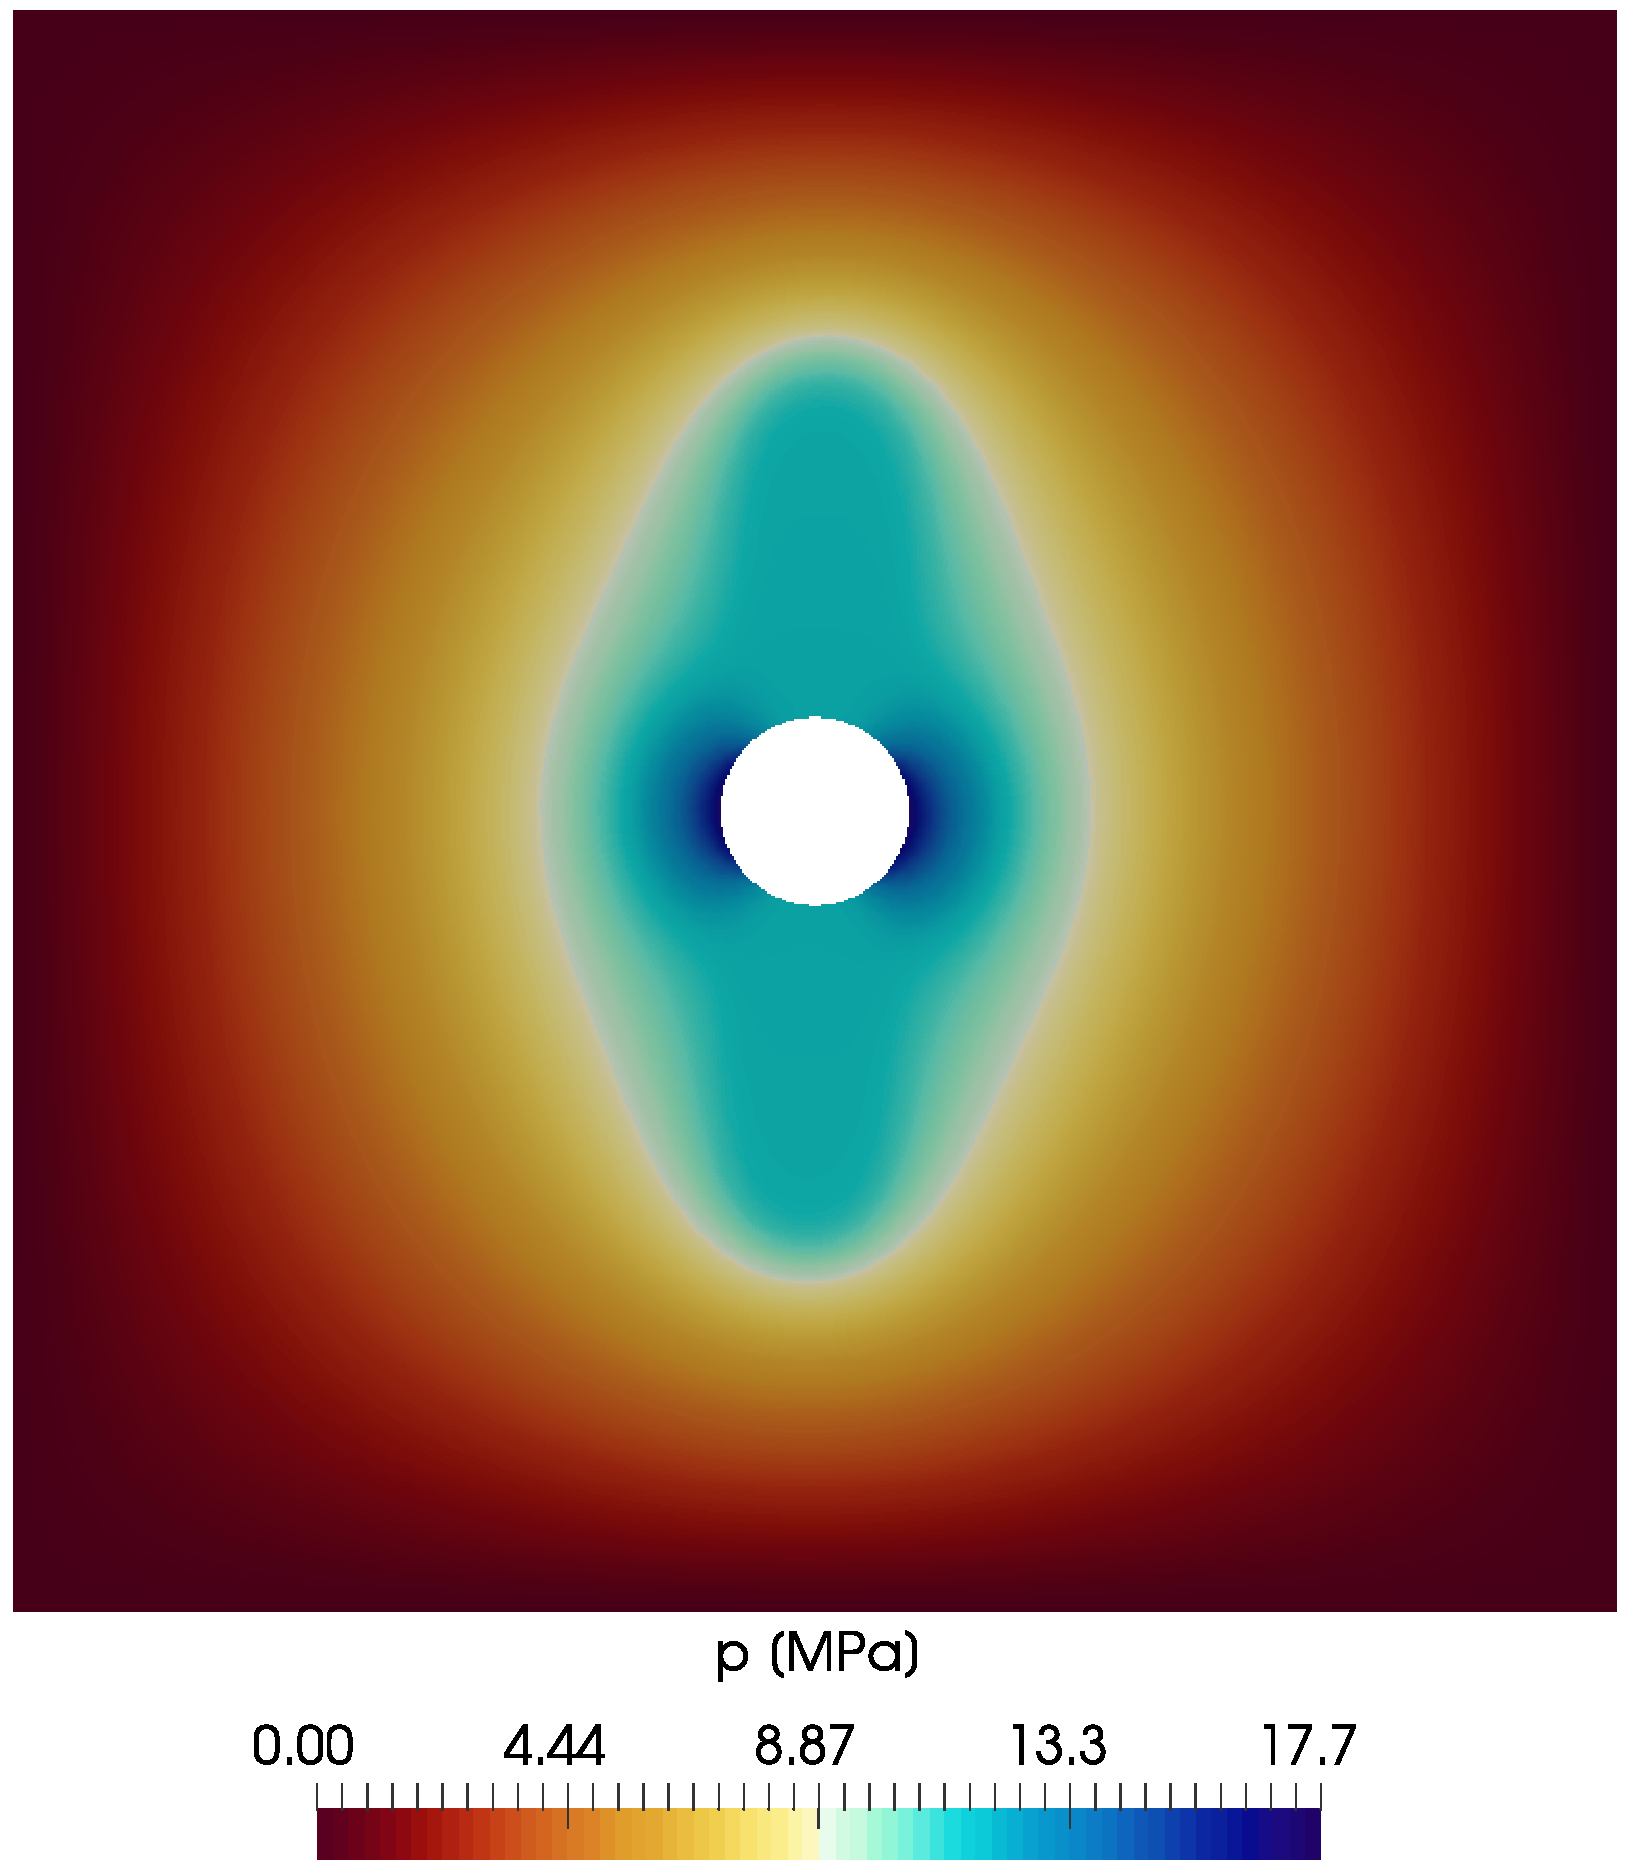
\includegraphics[width=60mm]{pressure49}\label{Fig:Gas_p_iii}}
\caption{Left: Phase field diagram at different stages (\ref{Fig:Gas_d_i}) $t=0.5t_f$, (\ref{Fig:Gas_d_ii}) $t=0.74t_f$, and (\ref{Fig:Gas_d_iii}) $t=t_f$). Right: Pressure profile at (\ref{Fig:Gas_p_i}) $t=0.5t_f$, (\ref{Fig:Gas_p_ii}) $t=0.74t_f$, and (\ref{Fig:Gas_p_iii}) $t=t_f$.}
\label{Fig:Gas_snapshots}
\end{figure}



%\todo[inline]{YS: The natural order is to first give OUR prediction of the breakdown pressure, then compare it with classical solutions.\\
%Vahid: The order is changed. See below.}

\begin{figure}
    \centering
    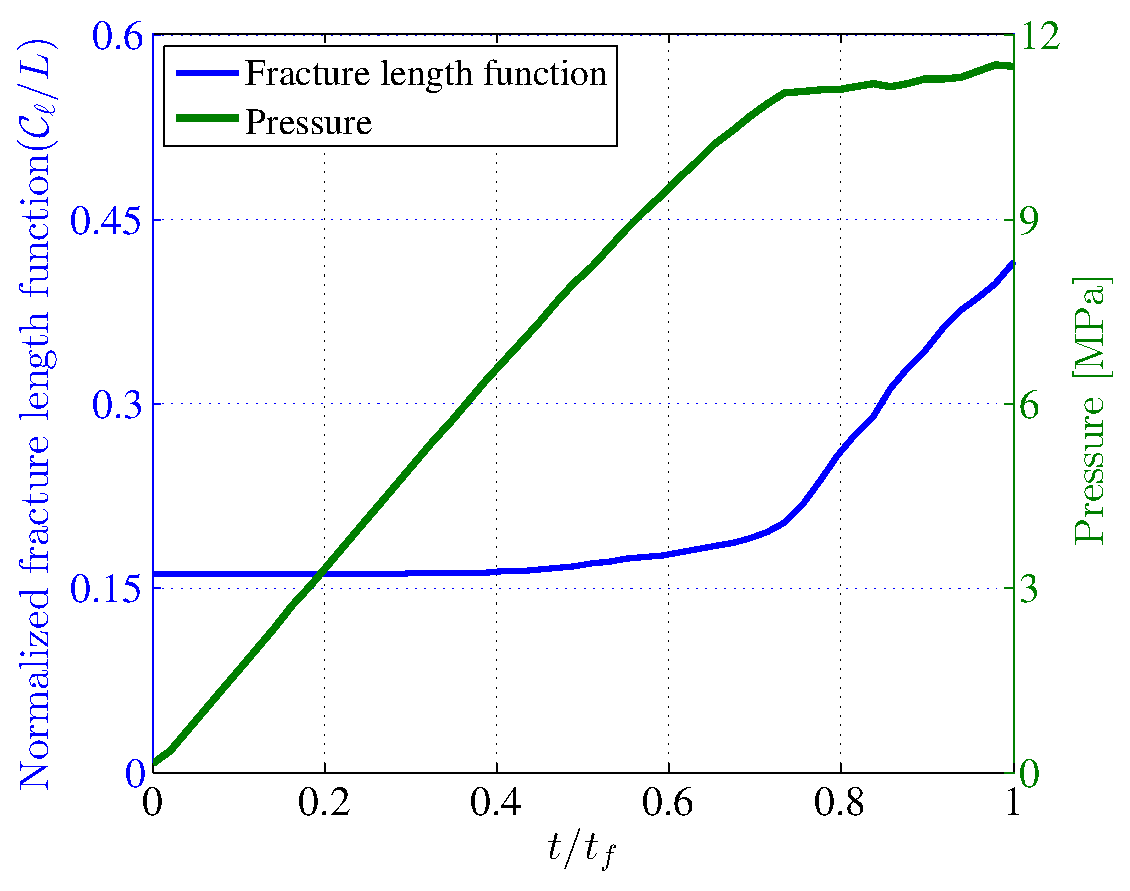
\includegraphics[width=0.6\textwidth]{Fracturelength_pressureboreholes_sigma_2}
    \caption{ The pressure at the top of the borehole (green line), and the fracture length function (blue line) as functions of time. The time when there is a sudden change of slope in $\mathcal{C}_{\ell}$ assumes the time corresponding to the breakdown pressure ($t=0.72t_f$) and the corresponding breakdown pressure is $p_b =10.9$ MPa. This is in agreement with H-F and H-W analytical solutions.}
	\label{Fig:Gas_pressure_Length_Sigma_i}
\end{figure}

Figure \ref{Fig:Gas_snapshots} shows the evolution of phase field diagram (left) and pressure profile (right) at different time steps. As seen, the fractures propagate along a straight line, and the pressure profile is accordingly distributed with the highest gradient around the borehole.

Next, we aim to calculate the breakdown pressure $p_b$, the pressure value when %at which the rapid drop in the injection pressure occurs and with 
the fractures start to propagate.
Figure \ref{Fig:Gas_pressure_Length_Sigma_i} illustrates the pressure evolution at the top of the borehole and the fracture length function. To estimate the breakdown pressure, first we output the fracture length with regard to \eqref{Eq:Gamma_ell}.  Then, we obtain the time when the slope suddenly changes in the fracture length function ($\mathcal{C}_{\ell}$), which is the time corresponding to the breakdown pressure (here $t\approx 0.72t_f$). Hence the breakdown pressure reads $p_b =10.9$ MPa. This value for $p_b$ is in agreement with H-F and H-W analytical solutions. Also, our results agree  with experiments results of Ishida \emph{et al.}~\cite{ishida2012acoustic} within 30\%, see Table \ref{Tab:preakdown_ISO_insitustress} and the next paragraph for more elaborations. 
%To validate our code we compare the numerical breakdown pressure with classical solutions$\cdots$
\begin{table}[htbp]
	\centering
	\caption{Breakdown pressure of numerical test and analytical solutions for $\sigma_1=\sigma_3=1$ MPa.}
	\begin{tabular}{l c c c c}
		\hline 
		& Numerical & H-F solution & H-W solution & Experimental \cite{ishida2012acoustic}  \\
		\hline 
		$p_b$ (MPa) & 10.9 & 11 &  9.1 & 8.44\\
		\hline      
	\end{tabular}
	\label{Tab:preakdown_ISO_insitustress}
\end{table}

\paragraph{Classical solutions of breakdown pressure} There exist two classical expressions to calculate the breakdown pressure. In the case without poroelastic effect the rock deformation does not penetrate into the pressurized fracture, the Hubbert-Willis (H-W) solution applies \cite{hubbert1972mechanics}:
\begin{equation*}
    p_b =3 \sigma_{3}- \sigma_{1}+\sigma_T,
\end{equation*}
in which the rock is assumed to be an elastic medium. When the porous medium is set, the Haimson-Fairhurst (H-F) solution is preferred \cite{haimson1967initiation}:
\begin{equation*}
    p_b=\dfrac{3\sigma_{3}- \sigma_{1}+\sigma_T+p_0}{1+\dfrac{\nu}{1-\nu}\alpha},
\end{equation*}
where we denote by $p_b$ the breakdown fluid pressure, $\sigma_{3}$, and $\sigma_{1}$ are the minimum and maximum principal stresses, respectively, and $\sigma_T$ is the rock's tensile strength.

\paragraph{Effect of $N$, $h$, and $\ell$ on the breakdown pressure}
Here we aim to study how the number of time steps $N$, the mesh size $h$, and the regularization length scale $\ell$ affect the value of breakdown pressure. As seen in Figure \ref{Fig:Gas_Pressure_parameters}, the plots show similar numerical results for the pressure evolution.

%\begin{figure}
%    \centering
%    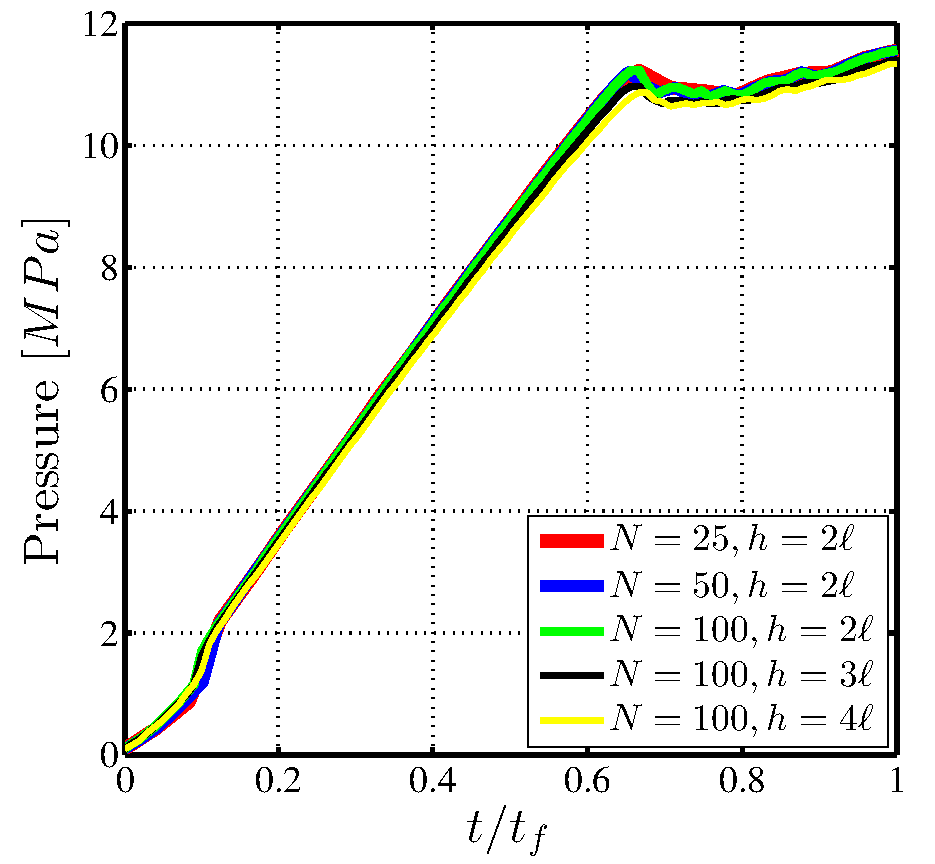
\includegraphics[width=0.6\textwidth]{breakdownpressure_diff_ell_loadstep}
%        \caption{The pressure profile at the top of borehole for different {time steps, $N$}, and $\ell$.}
%    \label{Fig:Gas_Pressure_parameters}
%\end{figure}


\begin{figure}
    \centering
    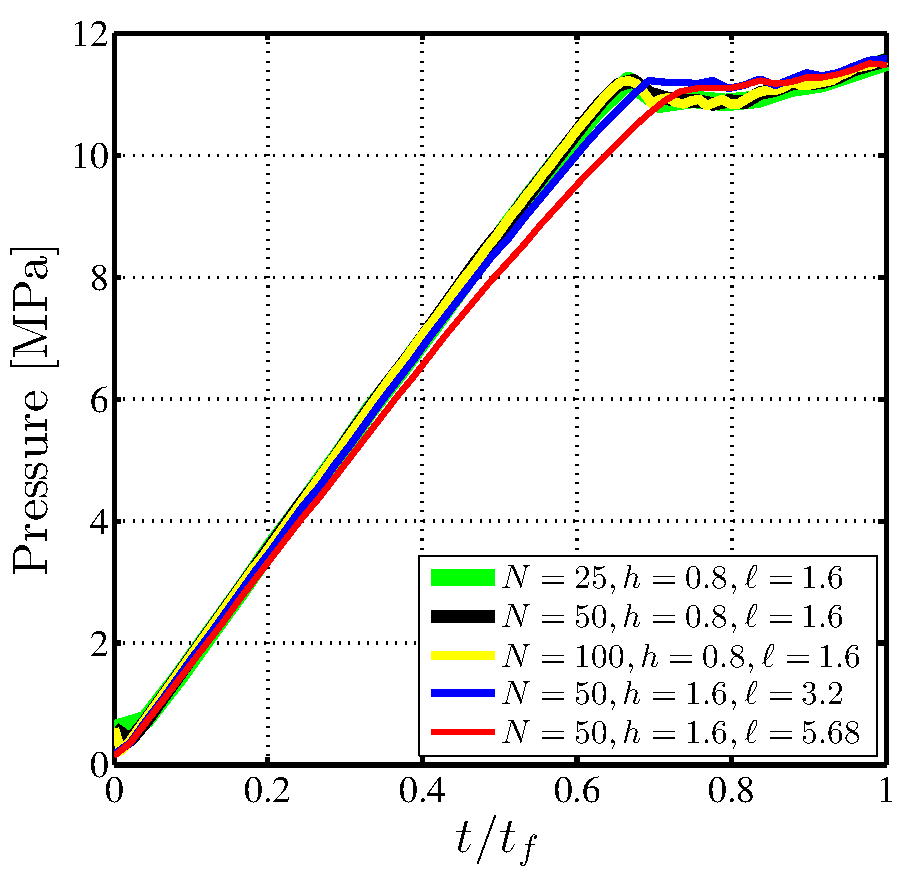
\includegraphics[width=0.6\textwidth]{breakdownpressure_diff_ell_loadstep_2}
        \caption{Evolution of the pressure at the top of the borehole for different numbers of time steps $N$, mesh size $h$, and $\ell$.}
    \label{Fig:Gas_Pressure_parameters}
\end{figure}

%\todo[inline]{YS: Effect of the deviatoric part of the \emph{in situ} stress?\\Vahid: Changed.}
\paragraph{Breakdown pressure result of an anisotropic \emph{in situ} stress} In this example we set the maximum ($\sigma_1=3$ MPa) and minimum ($\sigma_3=2$ MPa)  \emph{in situ} stress. The other input data and boundary conditions are the same as aforementioned.

The pressure at the top of the borehole and the fracture length function, \eqref{Eq:Gamma_ell}, at different stages are  illustrated in Figure \ref{Fig:Gas_pressure_Length_Sigma_diff}. The breakdown time ($t\approx 0.77t_f$) and the corresponding breakdown pressure is $p_b =11.9$ MPa, see Table \ref{Tab:preakdown_anISO_insitustress}.

\begin{table}[htbp]
    \centering
    \caption{Breakdown pressure of numerical test and analytical solutions for $\sigma_1=3$ MPa and $\sigma_3=2$ MPa.}
    \begin{tabular}{l c c c}
    \hline 
           & Numerical & H-F solution & H-W solution \\
    \hline 
           $p_b$ (MPa)& 11.9 & 14 &  9.8 \\
    \hline      
    \end{tabular}
    \label{Tab:preakdown_anISO_insitustress}
\end{table}

\begin{figure}[htbp]
    \centering
    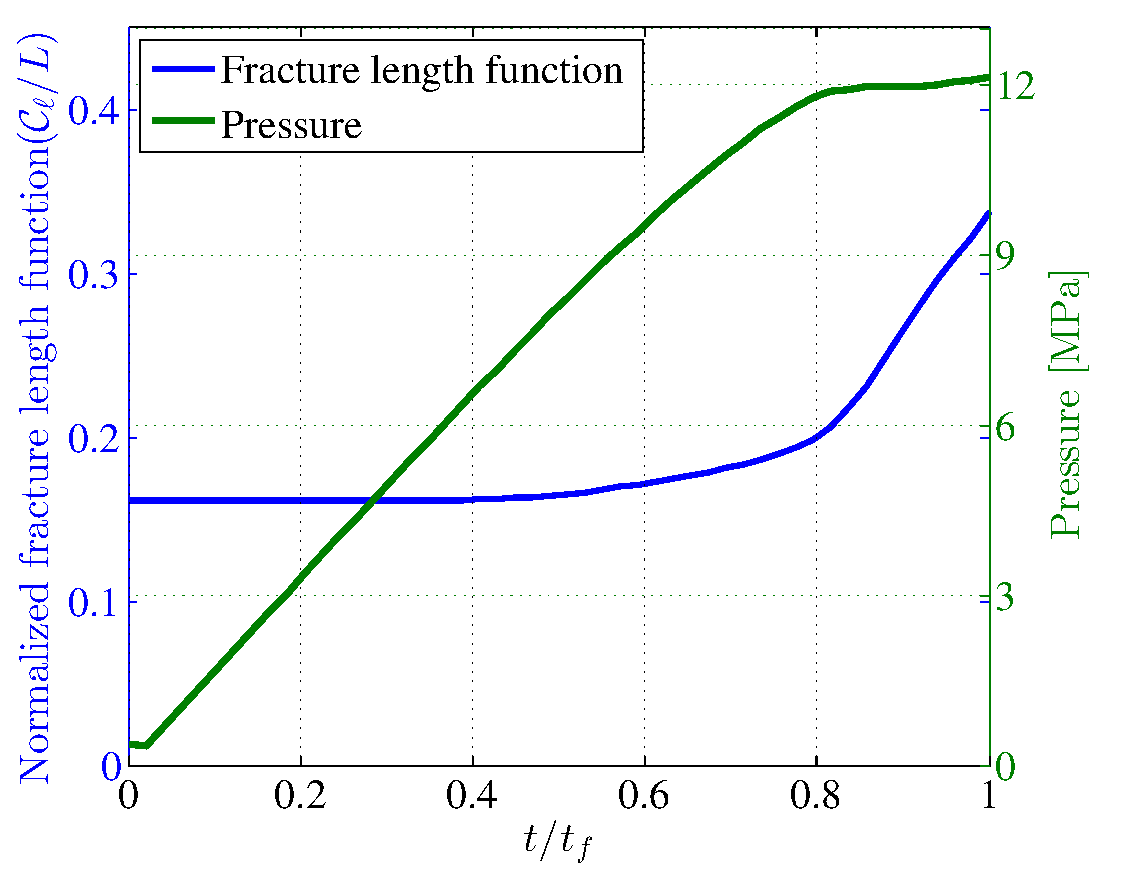
\includegraphics[width=0.6\textwidth]{Fracturelength_pressureboreholes_sigma_diff_2}
        \caption{The pressure at the top of the borehole (green line) and  the fracture length function (blue line) versus time for deviatoric \emph{in situ} stress are shown. The time ($t\approx 0.8t_f$) when there is a change of slope in the fracture length function ($\mathcal{C}_{\ell}$) should correspond to the breakdown pressure ($p_b=11.9$ MPa).}
    \label{Fig:Gas_pressure_Length_Sigma_diff}
\end{figure}

%\todo[inline]{Mostafa: Do we need keep this example? Since the results do not agree with experiments. Actually, the experiments indicate that the breakdown pressure is different for different fluids ($\mu$).\\Vahid: I added a few sentences to explain the case.}
\paragraph{Effect of dynamic viscosity on breakdown pressure} We conduct several numerical examples to investigate the effect of dynamic viscosity $\mu$ on the breakdown pressure $p_b$. 
In this set of examples an effective mesh size, the mesh size near the borehole or the fractures, $h\approx 1.6$ mm is adopted. Also, we set $\ell=2h$. In Figure \ref{Fig:Gas_Pressure_viscosity} we plot the pressure evolution up to the time when  $\mathcal{C}_\ell(t)$ changes slope, so that the end points correspond to the breakdown pressures. The results indicate that $p_b$ is approximately the same for different fluid viscosities, but the time when breakdown pressure reaches  is different. Figure \ref{Fig:Gas_Pressure_viscosity} demonstrates that the rock will break earlier for the fluid with bigger dynamic viscosity. Also it shows that regardless of the fracturing fluid, the breakdown pressure is slightly the same for all cases. This is in accordance with the physics that the breakdown pressure normally reflects the strength of the solid. However, Wang \emph{et al.}~\cite{wang2018influence} reported different breakdown pressures for different fluids which also agrees with some experiments \cite{ishida2012acoustic, ishida2016features}. We believe this discrepancy demands further research.

%\begin{figure}
%    \centering
%    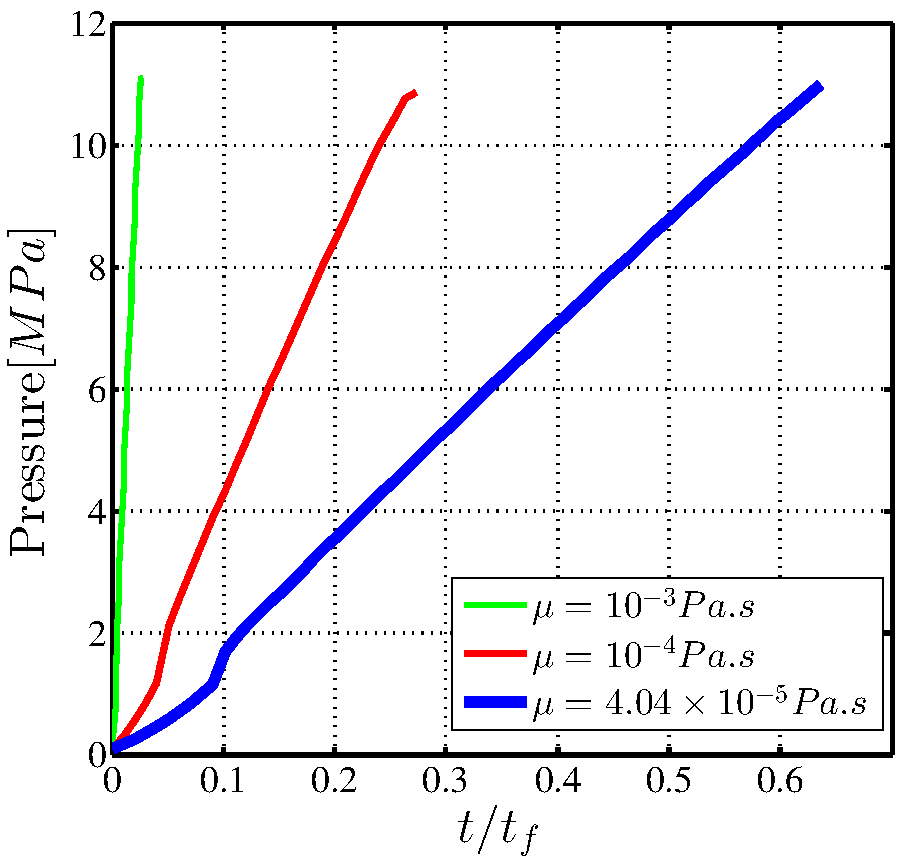
\includegraphics[width=0.6\textwidth]{breakdown_diff_viscosity}
%         \caption{The pressure profile at the top of borehole for different $\mu$. As seen, even though $p_b$ is the same for different fracturing fluids, by increasing $\mu$, the breakdown pressure is reached in earlier time.}
%    \label{Fig:Gas_Pressure_viscosity}
%\end{figure}

%\todo[inline]{YS: Problems with Figure \ref{Fig:Gas_Pressure_viscosity}: $t_c$ should be $t_f$, and also the second legend shall be $\mu=1.00\times10^{-4}$ Pa$\cdot$s.\\
%Mostafa: It's edited}

\begin{figure}[htbp]
    \centering
    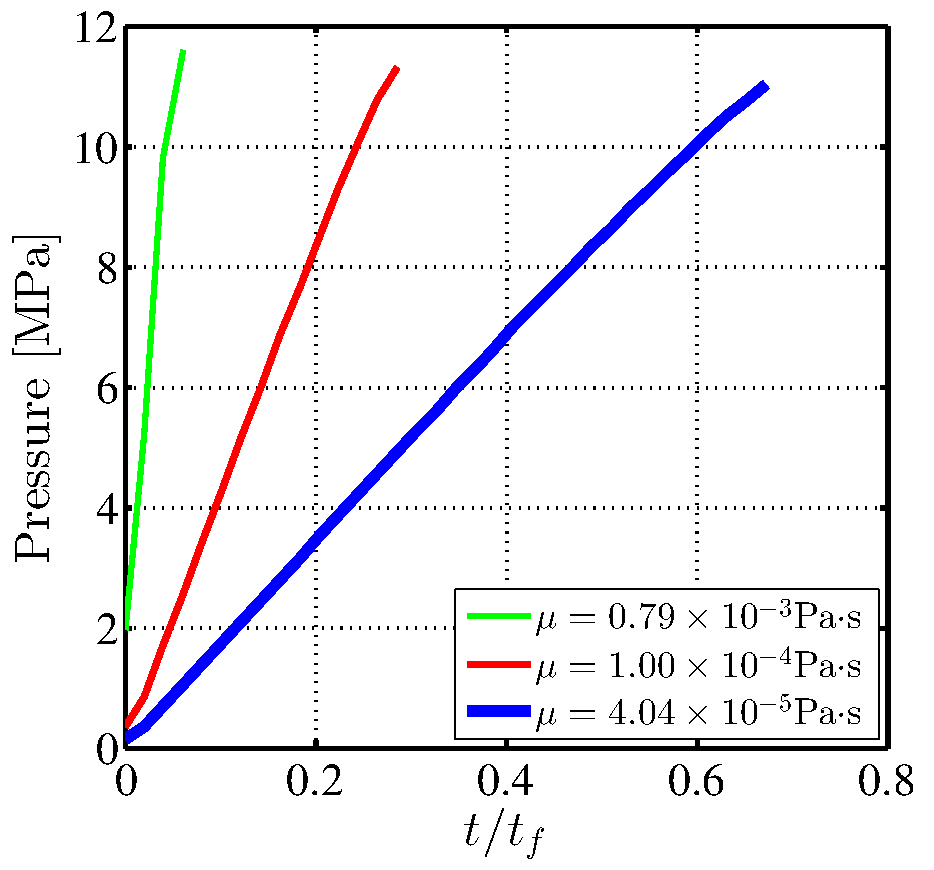
\includegraphics[width=0.6\textwidth]{breakdown_diff_viscosity_2}
         \caption{Evolution of the pressure at the top of the borehole for different $\mu$'s. As seen, even though $p_b$ is the same for different fracturing fluids, by increasing $\mu$, the breakdown pressure is reached earlier.}
    \label{Fig:Gas_Pressure_viscosity}
\end{figure}

\subsection{\added{Interaction between CO$_{2}$-driven fractures and natural fractures}} \label{sec: co2_interaction_inclined_ex}

\added{In this example, we investigate the interaction between two CO$_{2}$-driven fractures and two inclined natural fractures. The specimen has edge lengths of $L=170$ mm. The geometric setup and boundary conditions are depicted in Figure \ref{Fig:Gas_geometry_interaction}. The sample is discretized into 32,736 three-noded triangular elements so that the mesh size $h\approx 6.25 \times 10^{-1}$ mm is obtained. Also, we set $\ell=4h$. The remaining input data can be found in Table \ref{Tab:Gas_input}.}

\begin{figure}[htbp]
	\centering
	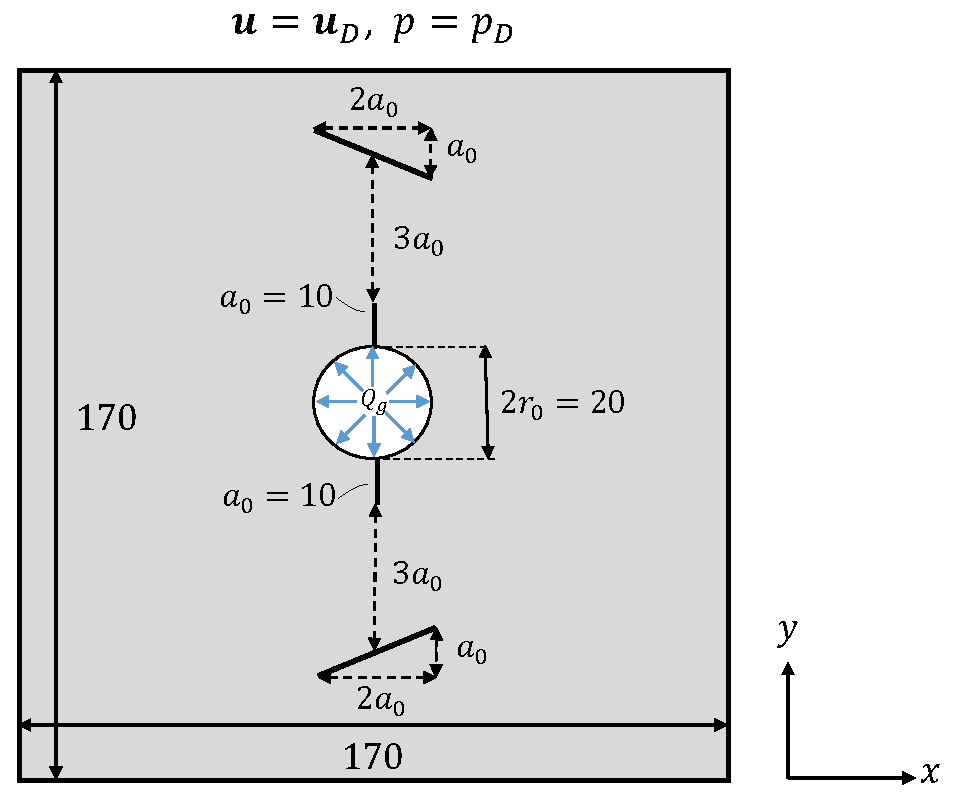
\includegraphics[width=0.8\textwidth]{GasFrackingModel2_inclined}
	\caption{\added{Interaction between CO$_{2}$-driven fracture and inclined natural fractures. The geometric setup and boundary conditions are shown (unit: mm). There exist two CO$_2$-driven fractures and two inclined natural ones.}}
	\label{Fig:Gas_geometry_interaction}
\end{figure}

\added{As in Figure \ref{Fig:Gas_geometry_interaction}, there exist two pre-existing vertical fractures representing the perforations and two inclined natural fractures. We set $d=1$ for both initial and inclined natural fractures, and the Dirichlet boundary condition $d=0$ is imposed on the external boundaries. The fluid is continuously injected into the central borehole with diameter $2r_0=20$ mm. The \emph{in situ} stress {with the value of $\sigma_1=\sigma_3=1$ MPa} is also imposed on the boundary by means of its `equivalent' prescribed displacement. See Section 4.5 for more descriptions.}

\added{Figure \ref{Fig:Gas_Inter_snapshots} shows the evolution of the phase field profile (left) and the pressure profile (right) at different time steps. As seen, the vertical fractures propagate along a straight line until $t=0.4t_f$. Then, near the inclined natural fractures, the CO$_2$-driven fractures turns to join them with an angle of approximately $90^{\circ}$ at $t=0.8t_f$. In the last frame \ref{Fig:Gas_Inter_d_iv}, the vertical fractures deviate into the inclined natural fractures and propagate from left tips. This fracture evolving pattern is called `crossing with an offset' which is one possible interaction process of hydraulic fracture and natural fracture \cite{yew2014mechanics}.}

\begin{figure}[htbp]
\centering %
\subfloat[]{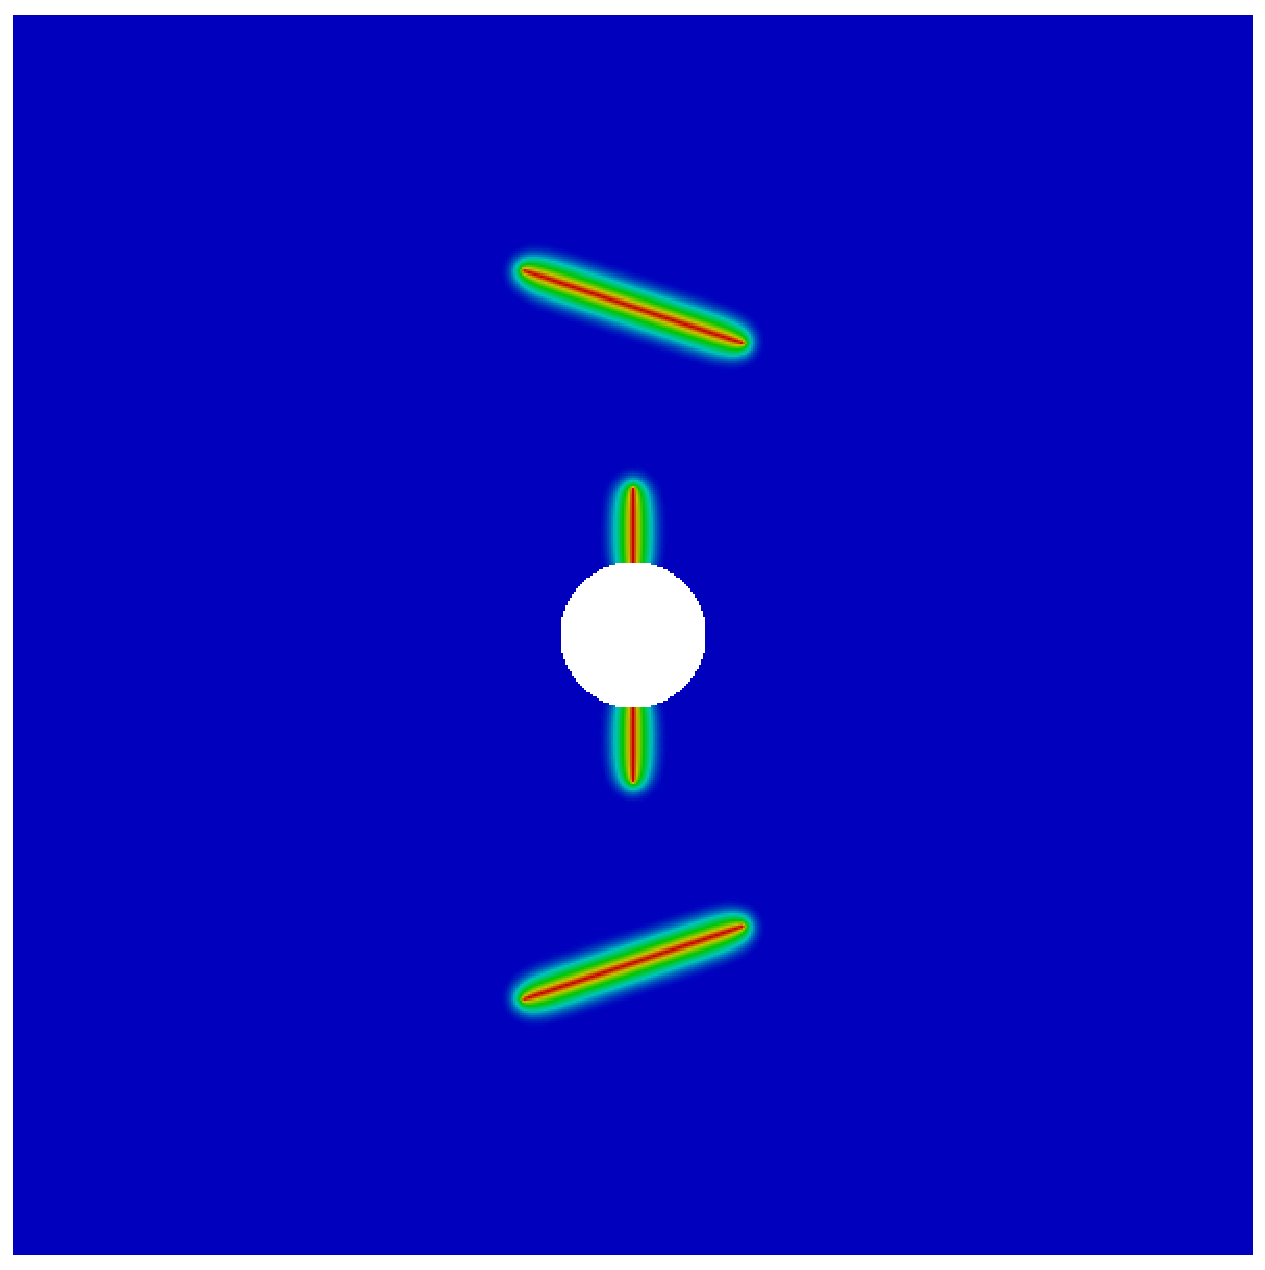
\includegraphics[width=42mm]{alpha1_inter_co2}\label{Fig:Gas_Inter_d_i}}
\subfloat[]{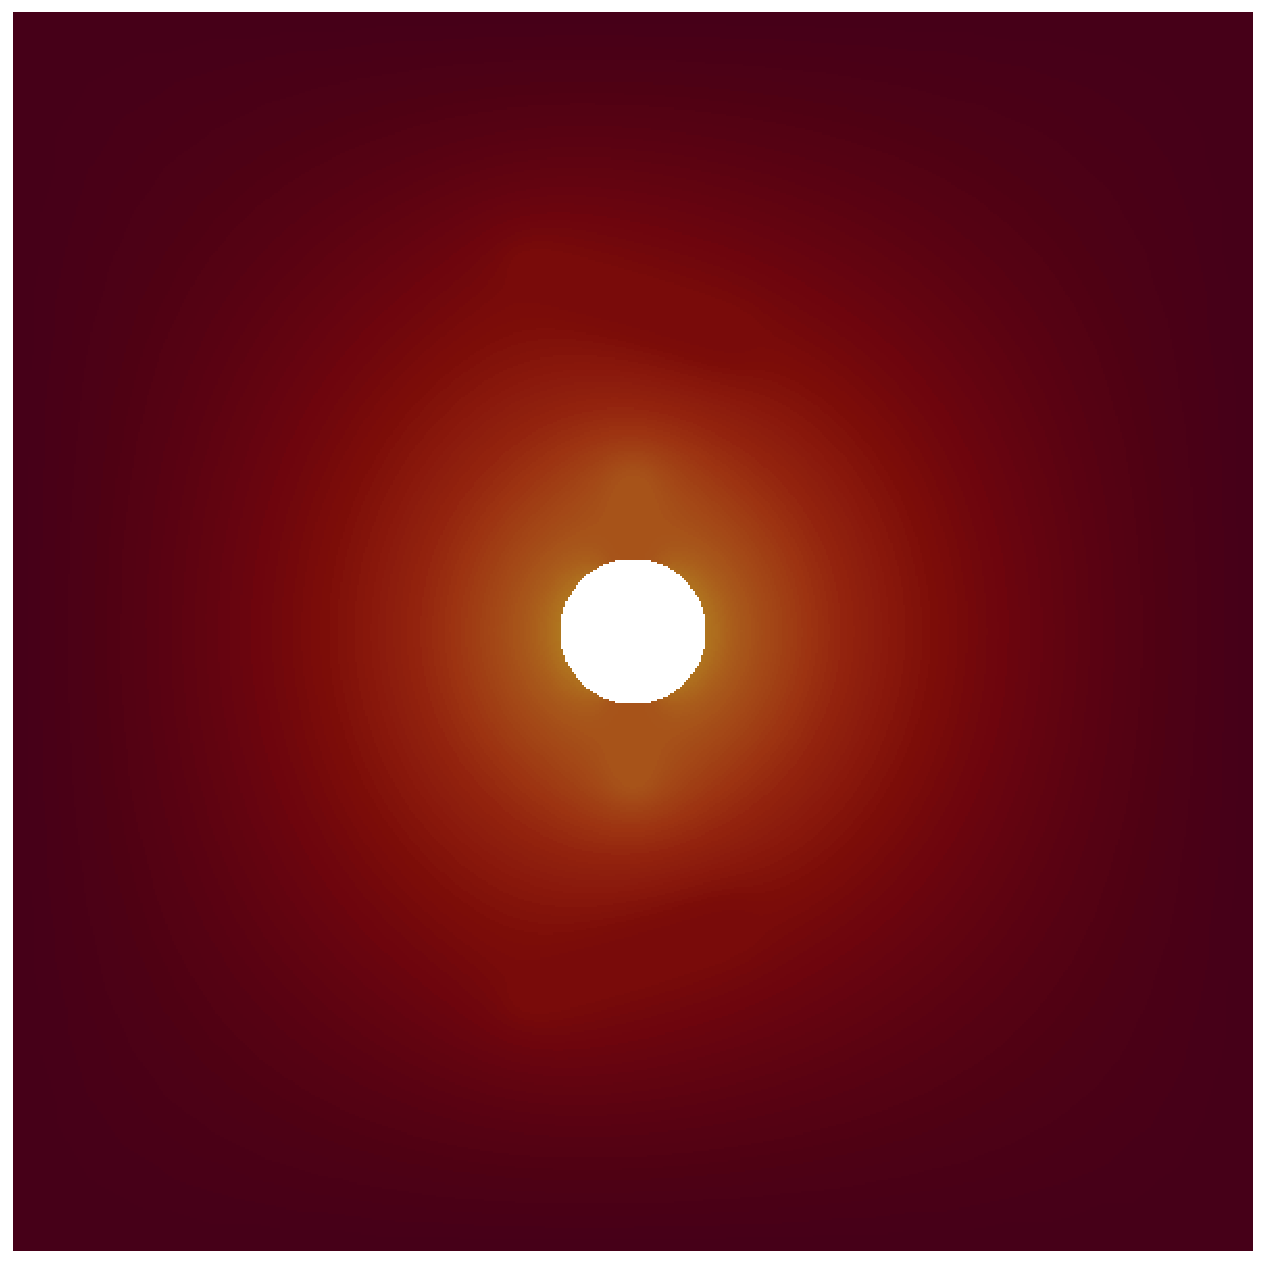
\includegraphics[width=42mm]{pressure1_inter_co2}\label{Fig:Gas_Inter_p_i}}\\
\subfloat[]{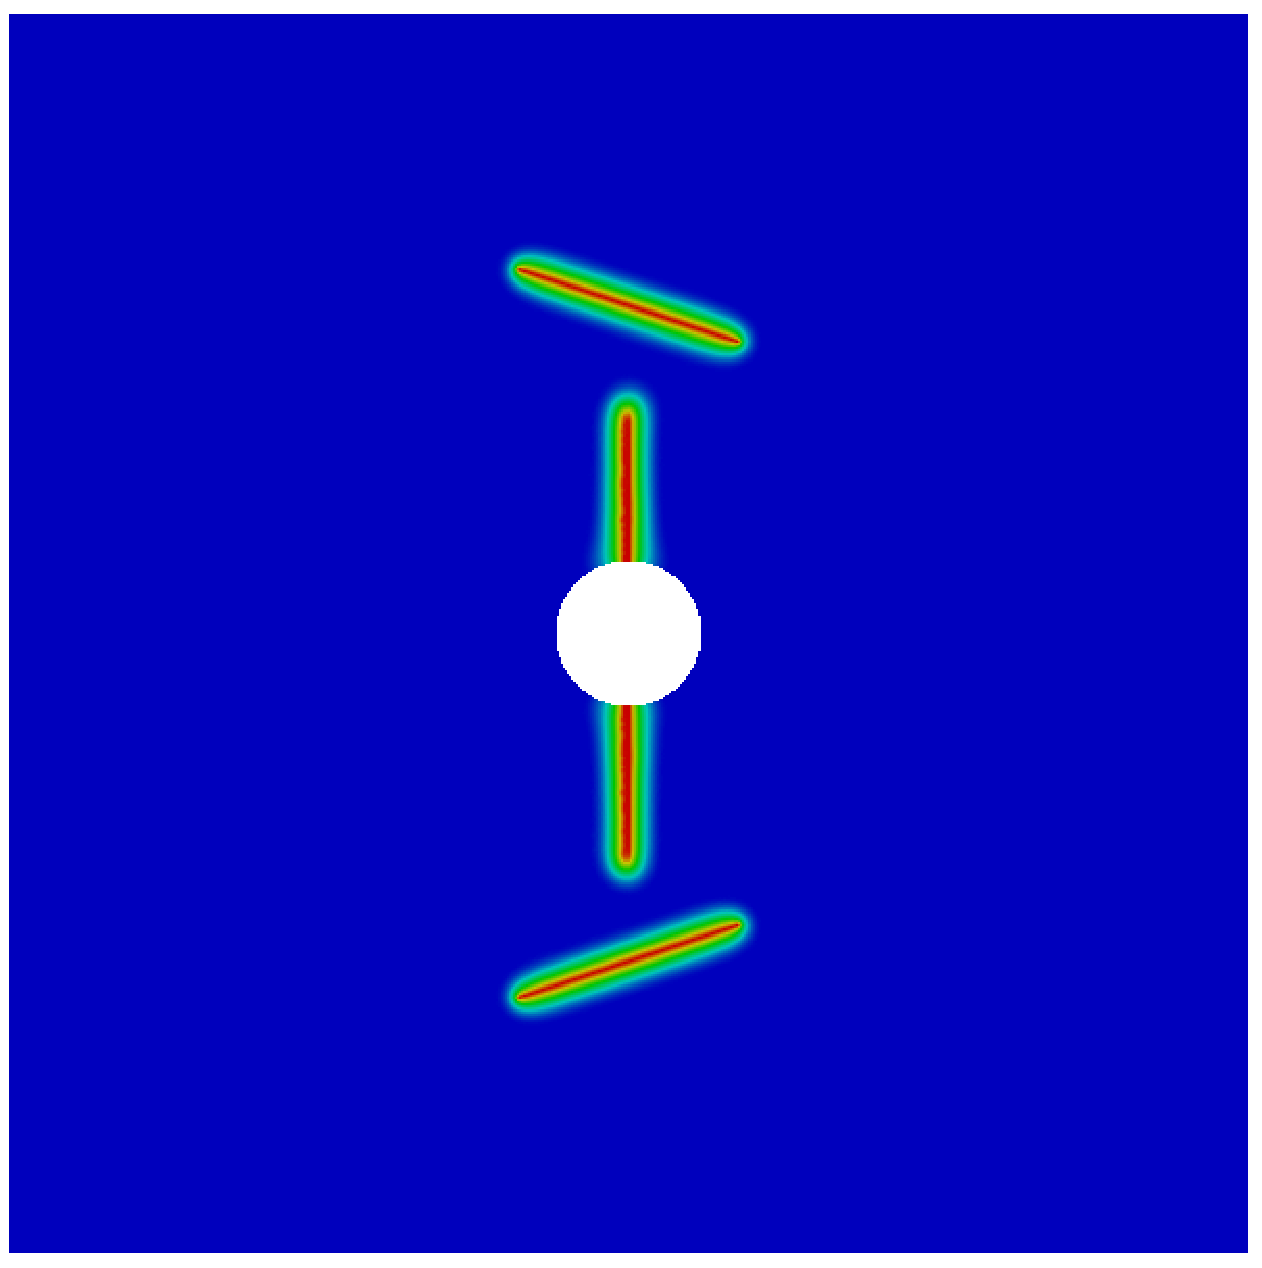
\includegraphics[width=42mm]{alpha2_inter_co2}\label{Fig:Gas_Inter_d_ii}}
\subfloat[]{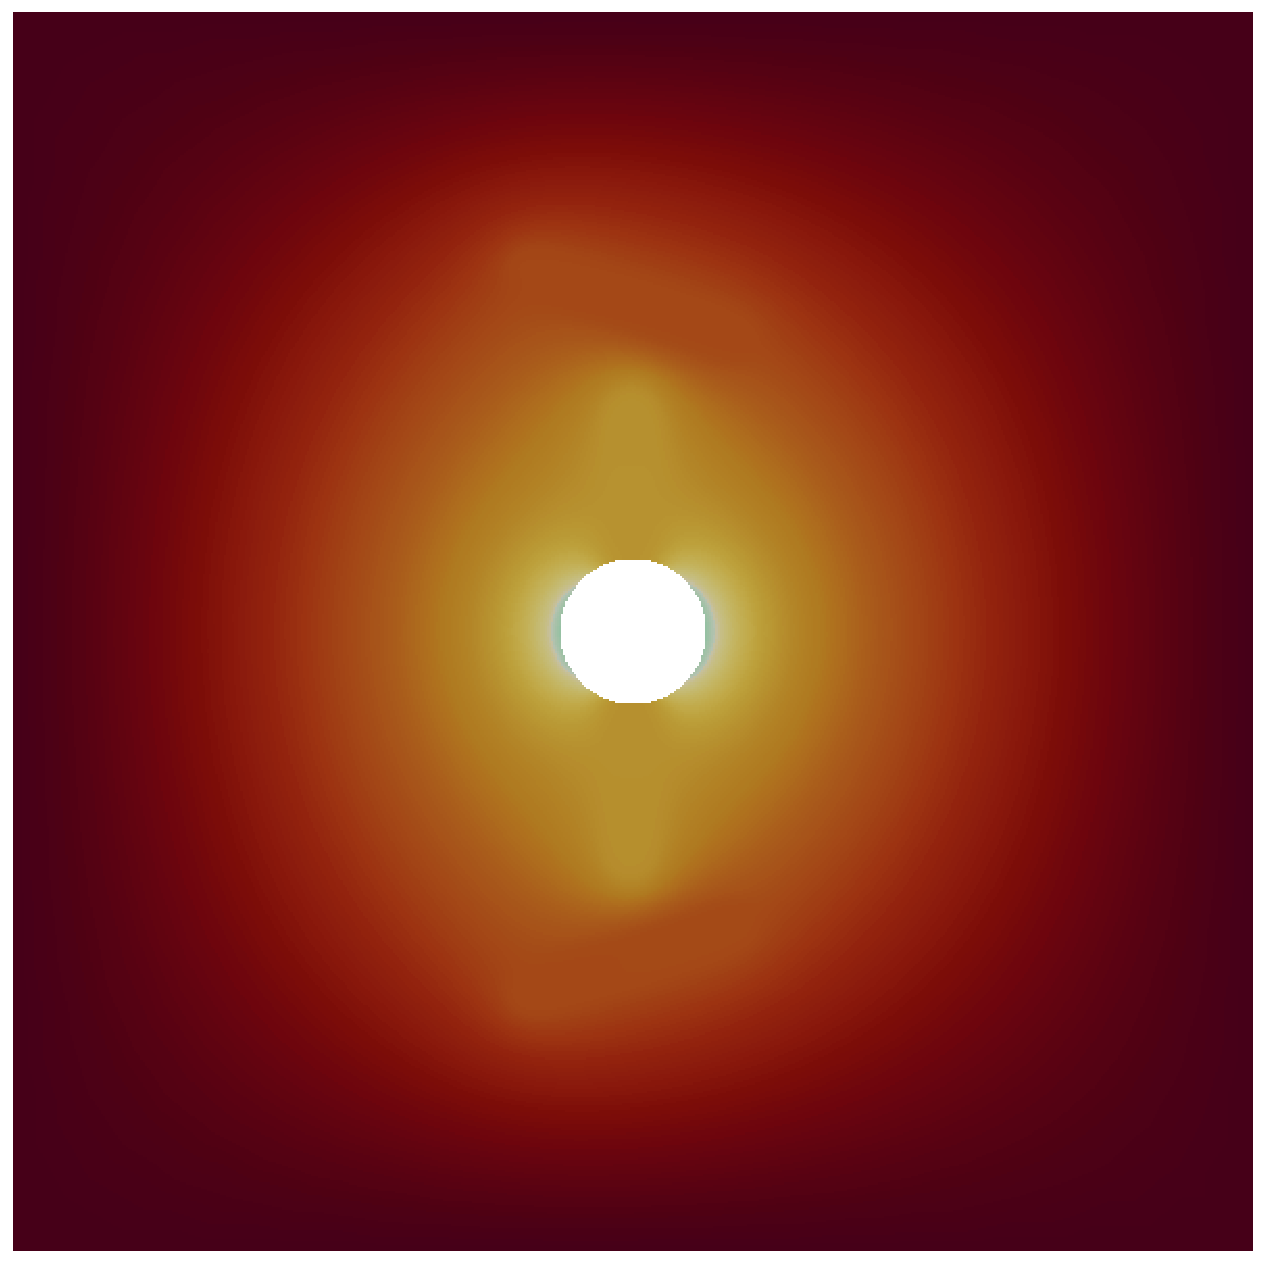
\includegraphics[width=42mm]{pressure2_inter_co2}\label{Fig:Gas_Inter_p_ii}}\\
\subfloat[]{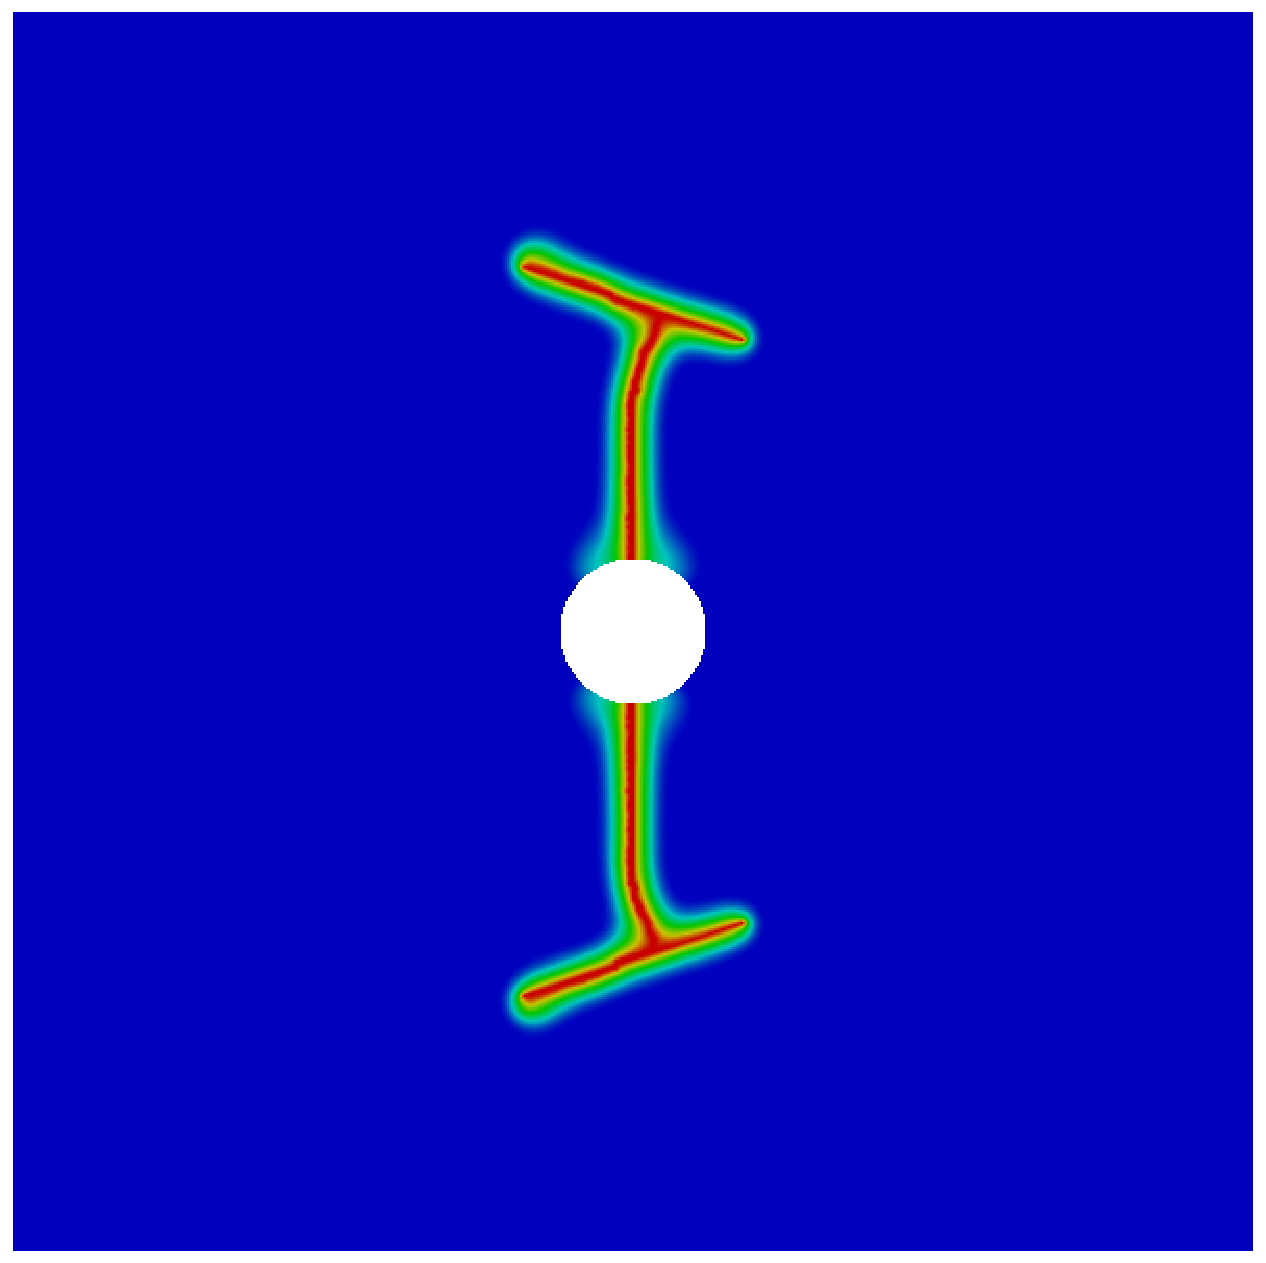
\includegraphics[width=42mm]{alpha4_inter_co2}\label{Fig:Gas_Inter_d_iii}}
\subfloat[]{\includegraphics[width=42mm]{pressure4_inter_co2}\label{Fig:Gas_Inter_p_iii}}\\
\subfloat[]{\includegraphics[width=42mm]{alpha5_inter_co2}\label{Fig:Gas_Inter_d_iv}}
\subfloat[]{\includegraphics[width=42mm]{pressure5_inter_co2}\label{Fig:Gas_Inter_p_iv}}
\caption{\added{Left: Phase field diagram at different stages (\ref{Fig:Gas_Inter_d_i}) $t=0.$, (\ref{Fig:Gas_Inter_d_ii}) $t=0.4t_f$, (\ref{Fig:Gas_Inter_d_iii}) $t=0.8t_f$, and (\ref{Fig:Gas_Inter_d_iv}) $t=t_f$. Right: Pressure profile at (\ref{Fig:Gas_Inter_p_i}) $t=0.$, (\ref{Fig:Gas_Inter_p_ii}) $t=0.4t_f$, (\ref{Fig:Gas_Inter_p_iii}) $t=0.8t_f$,  and (\ref{Fig:Gas_Inter_p_iv}) $t=t_f$. As seen, the vertical fractures propagate along a straight line until they reached the natural fractures. Then, they deviate into the inclined natural fractures, and continue evolving from left tips. `Crossing with an offset' is one possible interaction process of hydraulic fracture and natural fracture \cite{yew2014mechanics}.}}
\label{Fig:Gas_Inter_snapshots}
\end{figure}